\documentclass[10pt,a4paper]{article}
\usepackage[utf8]{inputenc}
\usepackage[T1]{fontenc}
\usepackage{amsmath}
\usepackage{amsfonts}
\usepackage{amssymb}
\usepackage{graphicx}
\usepackage{indentfirst}
\usepackage{etoolbox}
\usepackage{placeins}
\usepackage{subcaption}
\usepackage{gensymb}
\usepackage{siunitx}
\usepackage{svg}
\usepackage[hidelinks]{hyperref}
\usepackage[polish]{babel}

\usepackage[style=ieee, backend=bibtex ,sorting=none]{biblatex}
\addbibresource{refs.bib}
%opening
\author{Piotr Kumala}
\title{Zastosowanie rekurencyjnych sieci neuronowych do predykcji szeregów czasowych}
\date{}
\graphicspath{ {./img/} }
\renewcommand*\contentsname{Spis treści}
\renewcommand*\figurename{Rysunek}
\renewcommand*\tablename{Tabela}
\renewcommand*\tableautorefname{Tab.}
\renewcommand*\figureautorefname{Rys.}
\DeclareFieldFormat{urldate}{dostęp: #1}


\begin{document}
\begin{titlepage}
	\begin{center}
		
\includegraphics[width=0.4\textwidth]{img/university.jpg}
		\vspace*{1cm}
		
		{\Huge
			\textbf{Praca magisterska} \\
			
		}
		\vspace{0.5cm}
		{\Large
			Zastosowanie rekurencyjnych sieci neuronowych do predykcji szeregów czasowych
			
			\vspace{1cm}
			
			\textbf{Piotr Kumala} \\
		}
		\vspace{0.5cm}
		kierunek studiów: \textbf{Informatyka Stosowana} \\
		
		\vspace{1cm}
		
		{\Large Opiekun: \textbf{dr hab. inż. Piotr A. Kowalski, prof. AGH}}
		\vfill
		
		\
		\vspace{0.8cm}
		
		
		Wydział Fizyki i Informatyki Stosowanej\\
		Akademia Górniczo-Hutnicza im. Stanisława Staszica\\
		Kraków, wrzesień 2022 r.
		
	\end{center}
\end{titlepage}
\pagenumbering{gobble}
\newpage
\begin{center}
	\textbf{Oświadczenie studenta}
\end{center}

Uprzedzony o odpowiedzialności karnej na podstawie art. 115 ust. 1 i 2 ustawy z dnia
4 lutego 1994 r. o prawie autorskim i prawach pokrewnych (t.j. Dz. U. z 2018 r. poz. 1191 z
późn. zm.): „Kto przywłaszcza sobie autorstwo albo wprowadza w błąd, co do autorstwa całości
lub części cudzego utworu albo artystycznego wykonania, podlega grzywnie, karze
ograniczenia wolności albo pozbawienia wolności do lat 3. Tej samej karze podlega, kto
rozpowszechnia bez podania nazwiska lub pseudonimu twórcy cudzy utwór w wersji
oryginalnej albo w postaci opracowania, artystyczne wykonanie albo publicznie zniekształca
taki utwór, artystyczne wykonanie, fonogram, wideogram lub nadanie.”, a także uprzedzony o
odpowiedzialności dyscyplinarnej na podstawie art. 307 ust. 1 ustawy z dnia 20 lipca 2018r.
Prawo o szkolnictwie wyższym i nauce (Dz. U. z 2018 r. poz. 1668 z późn. zm.) „Student
podlega odpowiedzialności dyscyplinarnej za naruszenie przepisów obowiązujących w uczelni
oraz za czyn uchybiający godności studenta.”, oświadczam, że niniejszą pracę dyplomową
wykonałem osobiście i samodzielnie i nie korzystałem ze źródeł innych niż wymienione w
pracy. 

Jednocześnie Uczelnia informuję, że zgodnie z art. 15a ww. ustawy o prawie autorskim
i prawach pokrewnych Uczelni przysługuje pierwszeństwo w opublikowaniu pracy
dyplomowej studenta. Jeżeli Uczelnia nie opublikowała pracy dyplomowej w terminie 6
miesięcy od dnia jej obrony, autor może ją opublikować chyba, że praca jest częścią utworu
zbiorowego. Ponadto Uczelnia, jako podmiot, o którym mowa w art. 7 ust. 1 pkt 1 ustawy z
dnia 20 lipca 2018 r. — Prawo o szkolnictwie wyższym i nauce (Dz. U. z 2018 r. poz. 1668 z
późn. zm.), może korzystać bez wynagrodzenia i bez konieczności uzyskania zgody autora z
utworu stworzonego przez studenta w wyniku wykonywania obowiązków związanych z
odbywaniem studiów, udostępnić utwór ministrowi właściwemu do spraw szkolnictwa
wyższego i nauki oraz korzystać z utworów znajdujących się w prowadzonych przez niego
bazach danych, w celu sprawdzania z wykorzystaniem systemu antyplagiatowego. Minister
właściwy do spraw szkolnictwa wyższego i nauki może korzystać z prac dyplomowych
znajdujących się w prowadzonych przez niego bazach danych w zakresie niezbędnym do
zapewnienia prawidłowego utrzymania i rozwoju tych baz oraz współpracujących z nimi
systemów informatycznych.

\vfill
\
\begin{flushright}
	............................................................... \\
	(czytelny podpis)
\end{flushright}

\newpage
\pagenumbering{arabic}
\tableofcontents
\newpage

\section{Wprowadzenie i cel pracy}

\subsection{Wprowadzenie}
Sieci neuronowe są coraz powszechniej używane do rozwiązywania wielu problemów życia codziennego. Nawet w pozornie prostych urządzeniach takich jak telefony komórkowe zawierane są układy elektroniczne specjalizujące się w obliczeniach korzystających z sieci neuronowych \cite{appleNeuralEngine}. Taki rozwój technologiczny może zostać zastosowany do próby zrozumienia i szukania rozwiązań problemów życia codziennego. Jednym z szeroko występujących w świadomości społecznej problemów jest poziom zanieczyszczenia środowiska naturalnego i zmiany klimatu. Co roku na początku zimy media raportują o wysokim poziome zanieczyszczeń powietrza w polskich miastach \cite{airPollutionPoland}. Podejmowane są również działania mające na celu ograniczenie poziomu tychże zanieczyszczeń przez samorządy i instytucje centralne. Posiadanie wiarygodnych estymacji skali problemu i jego zmiany w czasie może oferować wymierne korzyści w usprawnianiu reakcji na wysokie poziomy zanieczyszczeń. W tej pracy podjęta zostanie próba stworzenia wiarygodnego modelu predykcyjnego poziomu zanieczyszczeń korzystającego z rekurencyjnych sieci neuronowych.

\subsection{Cel pracy}
Rekurencyjne sieci neuronowe są szeroko wykorzystywane i rozwijane przez największe firmy technologiczne. Są one stosowane między innymi do rozpoznawania pisma odręcznego i tekstu dyktowanego \cite{googleLSTM}. Mając na uwadze ilość wysiłku wkładanego w ulepszanie tychże sieci nasuwa się pytanie: jakie rezultaty będą one osiągać w innych zastosowaniach? W ramach tej pracy zbadana zostanie jakość predykcji szeregów czasowych płynących z modeli opartych na rekurencyjnych sieciach neuronowych. Zostaną one zestawione z klasycznymi metodami predykcyjnymi w celu stwierdzenia zasadności stosowania sieci neuronowych. Specjalna uwaga zostanie również poświęcona różnicom w jakości uzyskiwanych rozwiązań różnych architektur sieci oraz skalowalności modeli opartych na rekurencyjnych sieciach neuronowych. 

\newpage
\section{Wstęp teoretyczny}
\subsection{Szereg czasowy}
W ramach pracy podejmowane będą próby predykcji szeregu czasowego. Przed rozpoczęciem dalszych dywagacji należy zdefiniować samo pojęcie szeregu czasowego, aby uniknąć nieścisłości. Podążając za Głównym Urzędem Statystycznym szeregiem czasowym nazywamy ciąg obserwacji ilustrujący kształt zjawiska w kolejnych okresach czasu \cite{GUS}. Obserwacją można określić zbiór cech opisujących zjawisko w danym punkcie czasu. Rozumiejąc w taki sposób pojęcie szeregu czasowego można w prosty sposób określić cel systemu predykcyjnego. System ten powinien być w stanie przewidzieć wartość pewnej cechy w kolejnym punkcie czasu na podstawie poprzednich obserwacji. Można również określić, że predykcja będzie tym lepsza im bardziej zgodna z posiadanymi obserwacjami. 

\subsection{Regresja liniowa}
Jedną z najbardziej klasycznych metod predykcyjnych jest regresja liniowa. Jej podstawy zostały położone w pracach Legrende'a i Gauss'a na początku XIX wieku \cite{seal1967studies}. Polega ona na dopasowywaniu funkcji liniowej do danych w taki sposób, aby jak najlepiej opisywała ona kształt i właściwości danych. Najprostszym mechanizmem służącym do zapewnienia optymalnych wyników jest metoda najmniejszych kwadratów opisana po raz pierwszy przez Legrende'a w 1805 roku \cite{legendre1806nouvelles}. Polega ona na takim dopasowywaniu parametrów funkcji aby zminimalizować sumaryczny kwadrat odległości obserwacji od prostej opisanej funkcją. 

Na \autoref{figure:linear_example} przedstawione zostało przykładowe wykorzystanie regresji liniowej. Linia prosta dopasowana jest do zbioru danych oznaczonych punktami. Przykład ten obrazuje pewne niedogodności płynące z użycia metody najmniejszych kwadratów. Prosta powstała dzięki minimalizacji uśrednionego błędu lepiej odwzorowuje niektóre punkty od innych. Wartości znajdujące się bliżej średniej są o wiele lepiej reprezentowane w wyniku regresji. 
\begin{figure}[!ht]
	\centering
	\makebox[0pt]{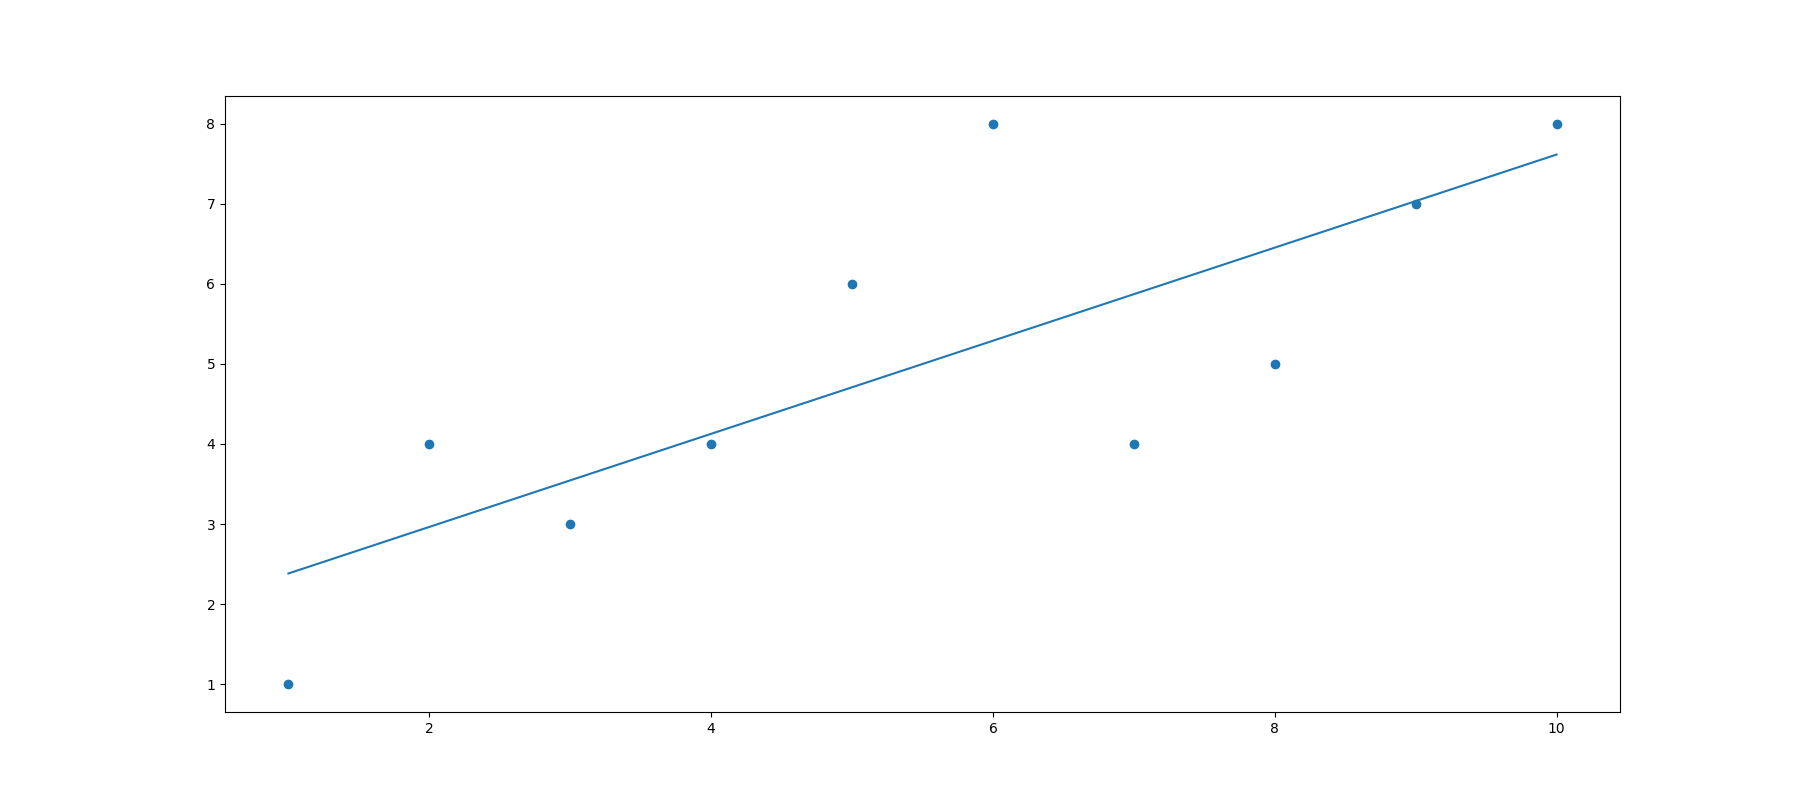
\includegraphics[scale=0.3]{example_linear_regression.png}}
	\caption{Przykład wyniku regresji liniowej}
	\label{figure:linear_example}
\end{figure}
\FloatBarrier

\subsection{Drzewa decyzyjne}
Jedną z najszerzej używanych metod uczenia maszynowego są drzewa decyzyjne. Są one powszechnie wykorzystywane ze względu na swoją prostotę oraz możliwość intuicyjnego zrozumienia wyników \cite{wu2008top}. Drzewem decyzyjnym nazywamy model predykcyjny, $h: X \rightarrow Y$, który przewiduje wartość $Y$ dla $x$ poprzez trawers drzewa od korzenia do liścia. Na każdym węźle drzewa kierunek przejścia jest wybierany poprzez rozdzielenie przestrzeni wejściowej. Najczęściej jest ono dokonywane na podstawie cech obserwacji $x$ \cite{books/daglib/0033642}. Wynikiem procesu uczenia jest drzewo pozwalające prześledzić ścieżkę jaką podąża każda obserwacja $x$ w celu przypisania jej odpowiedniej wartości. Przykładowe, bardzo uproszczone drzewo decyzyjne jest przedstawione na \autoref{figure:tree_example}.
\begin{figure}[!ht]
	\centering
	\makebox[0pt]{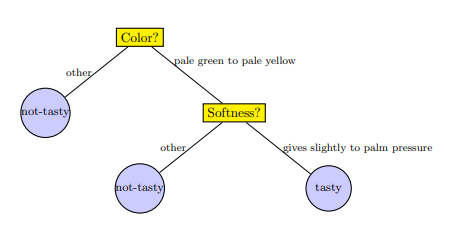
\includegraphics[scale=0.8]{example_decission_tree.png}}
	\caption{Przykładowe drzewo decyzyjne}
	\label{figure:tree_example}
\end{figure}
\FloatBarrier

Na podstawie tego przykładu można łatwo zaobserwować główną zaletę drzew decyzyjnych, mianowicie łatwość interpretacji uzyskanego drzewa. Podejmowanie decyzji poprzez odpowiadanie na pytania, które stale zawężają możliwe rozwiązania jest intuicyjnie zrozumiałe. Powodem tej łatwości zrozumienia może być bliskość procesu wyboru przez drzewo do ludzkiego procesu podejmowania decyzji. Niektórzy ludzie twierdzą, że drzewo decyzyjne powiela ludzkie schematy myślowe \cite{James2013}. 

Drzewa decyzyjne mogą być wykorzystywane w problemach regresyjnych, to znaczy dla ciągłej dziedziny rozwiązań $Y$. Należy jednak pamiętać, że w takim przypadku  należy uważać na możliwość zbytniego dopasowywania drzewa do danych trenujących. Problem ten objawia się stworzeniem zbyt szczegółowego drzewa, które nie generalizuje odpowiednio danych nieobecnych w zbiorze uczącym.

\subsection{Rekurencyjne sieci neuronowe}
Rekurencyjne sieci neuronowe to sieci neuronowe posiadające pętlę sprzężenia zwrotnego w swojej warstwie rekurencyjnej. Taka struktura pozwala im ,,zapamiętywać'' informacje przez pewien okres czasu i wykorzystywać w dalszych predykcjach \cite{reviewOfANN2018}. Umiejętność ta pozwala na założenie, że rekurencyjna sieć neuronowa powinna dobrze zachowywać się w predykcji szeregu czasowego dzięki ,,zapamiętywaniu'' wartości w poprzednich krokach czasowych. 

Podwaliny rekurencyjnych sieci neuronowych zostały stworzone w 1986 roku przez D. Rumelhart'a. Opisywał on sposób uczenia sieci neuronowych poprzez propagację wsteczną błędu \cite{rumelhart1986learning}. Zauważył on, że korzystając z tej metody uczenia można wypracować sieć, która rekurencyjnie wyznaczy wartości wag neuronów w swojej warstwie ukrytej. Potrzeba opracowania nowego sposobu uczenia wynikała z istnienia zadań niemożliwych do rozwiązania poprzez proste połączenie jednostek wejściowych z wyjściowymi.

Powszechnym sposobem myślenia o strukturze sieci neuronowych jest seria warstw składających się na sieć. Każda warstwa składająca się z pewnej liczby neuronów komunikuje się z następną warstwą aż do osiągnięcia warstwy wyjściowej zwracającej wynik sieci. 

W przypadku sieci rekurencyjnej nie jest tworzona seria warstw komunikujących się ze sobą, a jedna rekurencyjna warstwa zmieniająca się w czasie. W celu lepszego zrozumienia struktury i sposobu działania takiej sieci często dokonywany jest proces rozwijania w czasie warstwy rekurencyjnej.

\begin{figure}[!ht]
	\centering
	\makebox[0pt]{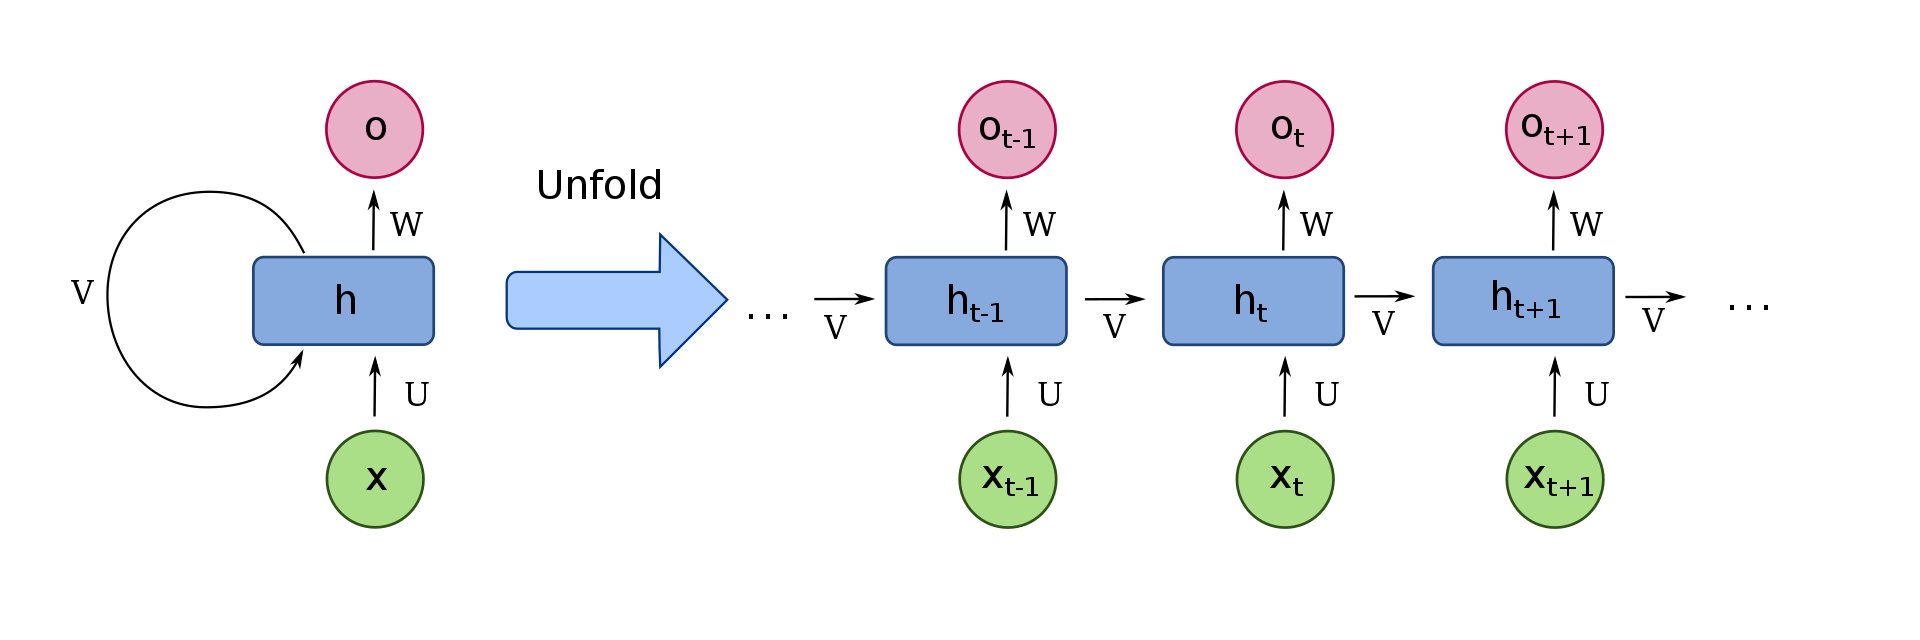
\includegraphics[scale=0.7]{Recurrent_neural_network_unfold.png}}
	\caption{Przykład rozwijania warstwy rekurencyjnej $h$}
	\label{figure:unfolded_rnn}
\end{figure}
\FloatBarrier

W powyższym przykładzie przedstawionym na \autoref{figure:unfolded_rnn} należy zauważyć, że w wersji rozwiniętej $h_{t-1}, h_t i h_{t+1}$ nie są osobnymi warstwami, a jedynie reprezentacją warstwy $h$ w różnych krokach czasowych. 

Na przestrzeni lat powstało wiele wariacji na temat architektury rekurencyjnych sieci neuronowych odpowiadających na różne problemy i stawiane im wymagania. W dalszym ciągu pracy przedstawione zostaną wybrane architektury, które mogą zostać wykorzystane do rozwiązania postawionego problemu predykcji szeregu czasowego.


\subsection{Architektura LSTM}
Sieci typu Long Short-Term Memory(LSTM) powstały jako próba rozwiązania problemów występujących w klasycznych sieciach rekurencyjnych. Problemy te dotyczyły w dużej mierze aspektu rekurencyjnych sieci neuronowych pozwalającego ,,zapamiętywać'' poprzednie kroki czasowe. Zauważono, że korzystając z mechanizmu propagacji wstecznej przesyłany do następnych kroków czasowych sygnał błędu (sposób sieci na ,,zapamiętanie'' poprzednich przypadków) ma tendencję do znikania lub eksplodowania. 

Zniknięciem sygnału błędu nazwać można sytuację, w której dąży on do zera w kolejnych krokach czasowych. Jest ona problemem w procesie uczenia, ponieważ może doprowadzić do bardzo dużego przedłużenia procesu lub nawet całkowicie uniemożliwić poprawne nauczenie sieci.

Eksplozją sygnału błędu nazywana jest sytuacja, w której dąży on do nieskończoności. Sytuacja ta jest niepożądana, ponieważ bardzo duży błąd przesyłany do następnych kroków czasowych oznacza, że sieć tak naprawdę niczego nie ,,zapamiętuje''. Może to prowadzić do oscylacji wag w sieci bez sygnału błędu stabilizującego wynik. 

Problemy te zostały podniesione przez S. Hochreiter'a w jego pracy doktorskiej, a następnie dokładniej opisane w roku 1991 we wspólnej pracy z J. Schmidhuber'em. 
W ramach artykułu ,,Long Short-Term Memory'' zaproponowali oni całkowicie nową architekturę rekurencyjnej sieci neuronowej dążącą do rozwiązania wyżej opisanych problemów \cite{hochreiter1997long}.

Stworzona została architektura oparta na komórkach pamięci i bramkach. Podstawową składową warstwy w tej architekturze jest komórka pamięci. Trzonem komórki jest rekurencyjna jednostka liniowa posiadająca Stałą Karuzelę Błędu (Constant Error Carousel), w skrócie CEC. Wartości CEC będą nazywane stanem komórki. Istnienie tego mechanizmu eliminuje problemy z sygnałem błędu, ponieważ zapewnia on, że lokalny błąd nie będzie się samoistnie zmieniał w kolejnych krokach czasowych.

Mechanizmem odpowiedzialnym za modyfikację stanu komórki są bramki: wejściowa i wyjściowa. Bramka wejściowa zajmuje się kontrolą przepływu nowych informacji do komórki. Oznacza to, że decyduje ona czy zachować obecny stan, czy nadpisać go nowymi informacjami. Można rozumieć zadanie bramki wejściowej jako określanie czy należy zapamiętać nową wiedzę lub uaktualnić istniejącą wiedzę. 

Bramka wyjściowa natomiast kontroluje przepływ stanu komórki na zewnątrz. Decyduje ona czy przechowywana przez komórkę wiedza jest warta przekazania innym komórkom do zapamiętania. Jej zadanie możemy rozumieć jako decyzję czy podzielić się swoją wiedzą z resztą komórek czy zachować ją dla siebie. 

\begin{figure}[!ht]
	\centering
	\makebox[0pt]{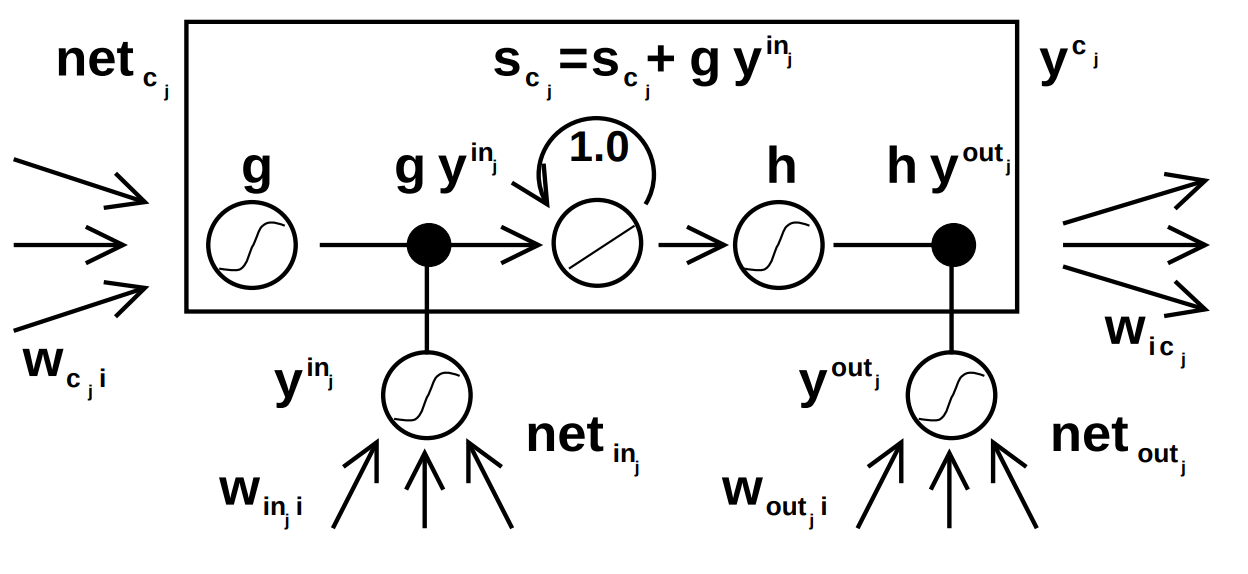
\includegraphics[scale=0.8]{lstm_without_forget_gate_schema.png}}
	\caption{Komórka pamięci w architekturze LSTM}
	\label{figure:lstm_architecture}
\end{figure}
\FloatBarrier

Na \autoref{figure:lstm_architecture} przedstawiony jest schemat budowy najprostszej komórki pamięci w sieci LSTM. Wyraźnie widoczne są bramki wejściowa i wyjściowa operujące na sygnałach wejściowych $w_{ini}$, $y^{in}$, $net_{in}$ oraz wyjściowych ${w_{outi}}$, $y^{out}$, $net_{out}$. Widoczny jest również mechanizm zmiany stanu wewnętrznego komórki $s_{c_j}$ na podstawie przepuszczonego przez bramkę wejściową sygnału $y_{in}$.

Stworzona w taki sposób architektura okazała się mieć jeden poważny problem. Stan komórki wykazywał tendencje do liniowego wzrostu w kolejnych krokach czasowych. Wzrost ten mógł prowadzić do saturacji funkcji h. Saturacja ta prowadziła do zaprzestania przyjmowania nowych błędów i zrównania wyniku komórki z wartością funkcji aktywacji bramki wyjściowej. W takich kierunkach komórka pamięci traciła swoje korzyści i wracała do zachowania typowego dla zwykłej sieci rekurencyjnej \cite{gers2000learning}.

Rozwiązaniem tego problemu okazało się dodanie trzeciej bramki nazywanej bramką zapominania. Zauważono, że przechowywanie w pamięci komórki danych przez bardzo długi często sprawia, że dane te są nieaktualne. Bramka zapominania kontroluje kiedy i ile przechowywanego stanu komórki $s_{c_j}$ należy zapomnieć. Dzięki usuwaniu z pamięci przestarzałych błędów wyeliminowany został problem saturacji funkcji h. Bramka zapominania stała się integralna częścią architektury LSTM. 

\begin{figure}[!ht]
	\centering
	\makebox[0pt]{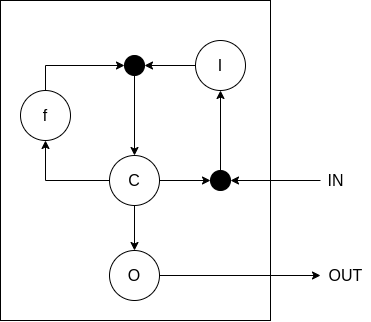
\includegraphics[scale=0.6]{lstm_with_forget_gate_schema.png}}
	\caption{Komórka pamięci w architekturze LSTM z bramką zapominania}
\end{figure}
\FloatBarrier
\newpage
\subsection{Architektura GRU}

Architektura Gated Recurrent Unit (GRU) została zaproponowana przez K. Cho w 2014 roku \cite{https://doi.org/10.48550/arxiv.1406.1078}. Oryginalnie została zaprojektowana do pracy w sieciach typu enkoder-dekoder do tłumaczenia tekstu jako alternatywa dla używanych wcześniej komórek z funkcją aktywacji tangens hiperboliczny. Decyzja o próbie wykorzystania jednostki rekurencyjnej działającej na bramkach była motywowana sukcesem sieci LSTM.

W porównaniu do architektury Long Short-Term Memory, Gated Recurrent Unit jest prostsza do zaimplementowania i mniej wymagająca obliczeniowo. Dzieje się tak dzięki zmniejszeniu ilości bramek kontrolujących pamięć komórki. Podczas gdy LSTM do poprawnego działania wymaga użycia trzech bramek (wejściowej, wyjściowej i zapominania) to wewnątrz jednostki GRU występują jedynie dwie bramki (aktualizacja i reset). 

\begin{figure}[!ht]
	\centering
	\makebox[0pt]{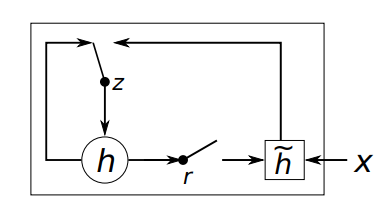
\includegraphics[scale=0.8]{gru_schema.png}}
	\caption{Komórka pamięci w architekturze GRU}
\end{figure}
\FloatBarrier

Na powyższym rysunku przedstawiony jest schemat komórki GRU, gdzie stan komórki w obecnym kroku czasowym $h$ zmienia się w $h'$. Widoczne są również bramki resetu $r$ i aktualizacji $z$. 

Bramka reset (reset gate) decyduje czy poprzedni wewnętrzny stan komórki powinien być zachowany czy odrzucony. Jej wartość w j-tej komórce w warstwie wyznaczamy ze wzoru:
\begin{equation}
	r_j = \sigma([W_rx]_j + [U_rh_{t-1}]_j),
\end{equation} 
gdzie $W_r$ i $U_r$ to macierze wag, których wartości są wyznaczane w trakcie uczenia sieci. Przy takich założeniach można zauważyć, że jeżeli wartość bramki reset będzie bliska zeru to stan komórki będzie często usuwany.

Bramka aktualizacji (update gate) decyduje natomiast jak duża część stanu z poprzedniego kroku czasowego powinna zostać zapamiętana w obecnym kroku. Wartość bramki w j-tej komórce warstwy wyznaczamy ze wzoru:
\begin{equation}
	z_j = \sigma([W_zx]_j + [U_zh_{t-1}]_j),
\end{equation} 
gdzie $W_z$ i $U_z$ to macierze wag analogiczne do tych występujących w bramce resetu. 

Wiedząc w jaki sposób zachowują się oba typy bramek oraz biorąc pod uwagę, że macierze $W_z, W_r, U_z, U_r$ są wyznaczane w trakcie uczenia można wysunąć kilka obserwacji. Dualizm bramek powinien prowadzić do jednej bramki będącej znacznie bardziej aktywnej od drugiej. Zjawisko to można rozumieć jako specjalizację komórek warstwy, gdzie te z aktywnymi bramkami resetu odpowiadają za pamięć krótkotrwałą, a te z aktywną bramką aktualizacji odpowiadają za pamięć długotrwałą. Pamiętając, że aktywność każdej bramki jest dopasowywana dla każdej komórki w procesie uczenia możemy założyć, że podział komórek na pamięć krótkotrwałą i długotrwałą będzie w wytrenowanej sieci rozłożony w sposób optymalny. Rozumiemy przez to, że jeżeli dane treningowe, na przykład nie wykazywały długofalowych trendów, a były bardziej chaotyczne i często zmieniające się to po procesie uczenia powinny dominować komórki z aktywną bramką resetu.

\newpage
\section{Zagadnienie predykcji zanieczyszczenia powietrza}
Odpowiednie dane są niezbędne w celu zbadania użyteczności rekurencyjnych sieci neuronowych do predykcji szeregów czasowych. Z tego powodu w celu stworzenia badawczo ciekawych szeregów czasowych przeznaczona została adekwatna ilość czasu. Przeanalizowano wiele możliwych zbiorów danych aby ich użyć do zbudowania szeregów czasowych. Ostatecznie podjęta została decyzja o połączeniu danych klimatycznych agregowanych przez Instytut Meteorologii i Gospodarki Wodnej oraz danych o zanieczyszczeniu powietrza zbieranych przez Główny Inspektorat Ochrony Środowiska. Oba te zbiory, sposób połączenia ich w szereg czasowy i napotkane trudności zostaną opisane w tym rozdziale. 

\subsection{Baza danych Instytutu Meteorologii i Gospodarki Wodnej}
Instytut Meteorologii i Gospodarki Wodnej to instytucja zajmująca się prognozowaniem pogody i sporządzaniem ekspertyz meteorologicznych. Cel ten jest realizowany między innymi poprzez przeprowadzanie systematycznych pomiarów i obserwacji korzystając z sieci stacji pomiarowych \cite{imgwTask}. Ten aspekt działalności Instytutu implikuje istnienie obszernej bazy danych pomiarowych, które są udostępniane publicznie ponieważ celem Instytutu jest służba społeczeństwu. Ten zbiór danych pomiarowych został wykorzystany do budowy szeregów czasowych. 

Publicznie dostępne są dane klimatyczne od 1951 roku do chwili obecnej. Są one udostępniane w formie dwóch plików csv dla każdego miesiąca roku. Dane w obu plikach mają analogiczną strukturę wyglądającą następująco:
\begin{center}
	\begin{tabular}{|c|c|c|c|c|c}
		Kod stacji & Nazwa stacji & Rok & Miesiąc & Dzień & Wyniki pomiarów...
	\end{tabular}
\end{center}
W kolejnych wierszach są zapisane informacje o pomiarach z jednej stacji z całego miesiąca, potem następnej i tak dalej. Ponieważ wyniki pomiarów z obu plików mogą mieć znaczenie w procesie predykcyjnym, podjęta została decyzja o korzystaniu z danych zapisanych w obu plikach. Biorąc pod uwagę oba pliki w bazie danych agregowane są wyniki pomiarów: 
\begin{itemize}
	\item Średniej dobowej temperatury [$\degree C$]
	\item Średniej dobowej wilgotności względnej [\%]
	\item Średniej dobowej prędkości wiatru [$\frac{m}{s}$]
	\item Średniego dobowego zachmurzenia ogólnego [oktany]
	\item Maksymalnej temperatury dobowej [$\degree C$]
	\item Minimalnej temperatury dobowej [$\degree C$]
	\item Temperatury minimalnej przy gruncie [$\degree C$]
	\item Sumy dobowej opadów [$mm$]
	\item Rodzaju opadu [S (Śnieg) /W (Deszcz)]
	\item Wysokości pokrywy śnieżnej [$cm$]
\end{itemize}
Na \autoref{figure:imgw} przedstawione zostały wartości średniej dobowej temperatury w latach 2001-2020. Na osi X reprezentowany jest czas w dniach, a na osi Y temperatura w stopniach Celsjusza. Wyraźnie widoczna jest okresowość danych zgodna z cyklem pór roku.  

Dla każdego pomiaru zapisywany jest również jego status pozwalający stwierdzić czy został on przeprowadzony poprawnie i czy dane zjawisko występowało w danym dniu. W wykorzystywanych danych z okresu 2001-2020 nie było przypadku błędnego pomiaru co pozwala wierzyć w dokładność danych i skrupulatność przeprowadzanych obserwacji. 


\begin{figure}[!ht]
	\centering
	\makebox[0pt]{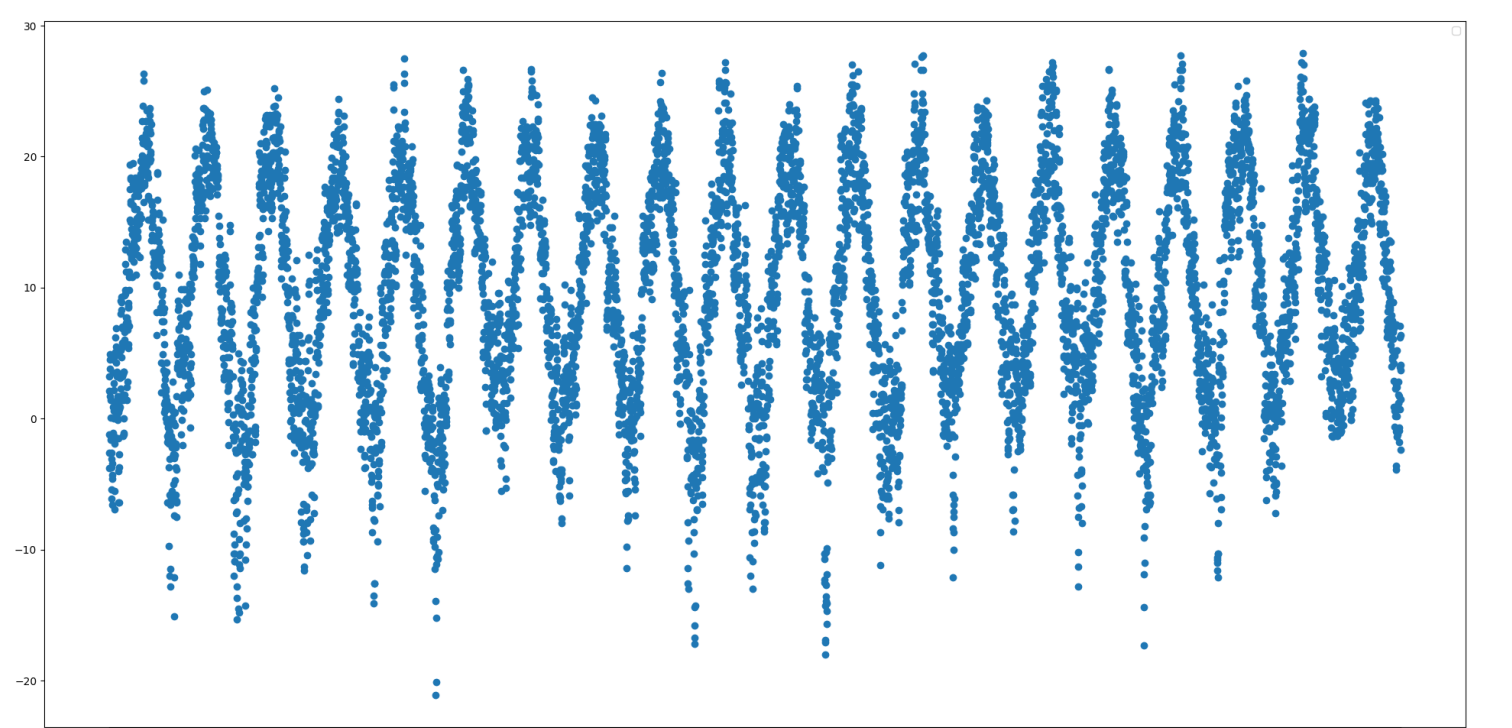
\includegraphics[scale=0.3]{imgw_description_krakow.png}}
	\caption{Średnia temperatura dobowa w latach 2001-2020}
	\label{figure:imgw}
\end{figure}
\FloatBarrier

\subsection{Baza danych Głównego Inspektoratu Ochrony Środowiska}
Główny Inspektorat Ochrony Środowiska to instytucja powołana 27 kwietnia 2001 roku \cite{giosStart}. Jako część swojej misji określa ona mierzenie stanu zanieczyszczenia środowiska oraz udostępnianie wyników tych pomiarów społeczeństwu \cite{giosMission}. Ten aspekt działalności Inspektoratu gwarantuje istnienie dużej bazy wyników pomiarów danych dotyczących poziomu zanieczyszczeń powietrza, które mogą zostać wykorzystane do tworzenia szeregów czasowych. 

Główny Inspektorat Ochrony Środowiska jest instytucją znacznie młodszą o Instytutu Meteorologii i Gospodarki Wodnej, więc dane agregowane przez Inspektorat nie będą dotyczyć tak długiego okresu czasu jak dane Instytutu. Jako że Główny Inspektorat Ochrony Środowiska jest instytucją względnie młodą to w jego początkowych stadiach nie monitorował on wielu różnych typów zanieczyszczeń oraz nie posiadał szerokiej sieci punktów pomiarowych. W trakcie jego rozwoju dochodziło również do zmian w formacie udostępnianych danych. Czynniki te musiały być brane pod uwagę w trakcie pracy z udostępnianymi przez niego danymi. 

Dane te są udostępniane w formie plików formatu xlsx, gdzie dla każdej substancji zanieczyszczającej tworzony jest osobny plik z wynikami pomiarów. Co do zasady struktura danych prezentuje się następująco:
\begin{center}
	\begin{tabular}{|c|c|c}
		Data wykonania pomiaru & Kod stacji 1 & Kod stacji 2 ...
	\end{tabular}
\end{center}
Różne czynniki zanieczyszczające mają również różne rozdzielczości czasowe, dla niektórych jest rozdzielczość godzinna, dla innych dobowa, dla niektórych są dostępne obie. 

Ilość badanych substancji zanieczyszczających powietrze fluktuuje w czasie. W pierwszym roku, dla którego dostępne są dane, mianowicie roku 2000 mierzone były:
\begin{itemize}
	\item Średnie dobowe stężenie Benzo(a)pirenu w pyle PM10
	\item Średnie dobowe stężenie Benzenu
	\item Średnie dobowe stężenie Kadmu w pyle PM10 
	\item Średnie dobowe stężenie Niklu w pyle PM10
	\item Godzinne stężenie Dwutlenku azotu
	\item Średnie dobowe stężenie Dwutlenku azotu
	\item Godzinne stężenie mieszaniny Tlenku azotu i Dwutlenku azotu
	\item Godzinne stężenie Ozonu
	\item Średnie dobowe stężenie pyłu PM10
	\item Godzinne stężenie Dwutlenku siarki
	\item Średnie dobowe stężenie Dwutlenku siarki
\end{itemize}
W kolejnych latach liczba badanych czynników zanieczyszczających oraz rozdzielczość czasowa tych badań znacząco wzrastała, jednak aby zachować możliwość budowy jak najdłuższego szeregu czasowego podjęta została decyzja o braniu pod uwagę jedynie polutantów występujących w wynikach pomiarów ze wszystkich lat działania Inspektoratu. 


Nie bez znaczenia jest również fakt, że ilość stacji badających różniła się znacznie pomiędzy różnymi substancjami. Ostatecznie wybrane zostało używanie jedynie średniego dobowego stężenia pyłu PM10, jako że był on badany przez największą ilość stacji przez najdłuższy możliwy czas. Czynniki te miały duży wpływ na proces budowania jednego szeregu czasowego na podstawie obu opisanych zbiorów danych, który zostanie opisany w dalszej części pracy.

Na \autoref{figure:gios} przedstawiony jest poziom zanieczyszczenia pyłem PM10 na terenie Krakowa w latach 2001-2020. Na osi x reprezentowany jest czas w dniach, a na osi y poziom zanieczyszczenia w $\frac{\si{\micro\gram}}{\si\meter^3}$. Różnymi kolorami przedstawione są wyniki z różnych stacji pomiarowych leżących na obszarze Krakowa. Wyraźnie widoczna jest potrzeba korzystania z więcej niż jednej stacji pomiarowej do stworzenia stałego ciągu obserwacji w analizowanym okresie. 
\begin{figure}[!ht]
	\centering
	\makebox[0pt]{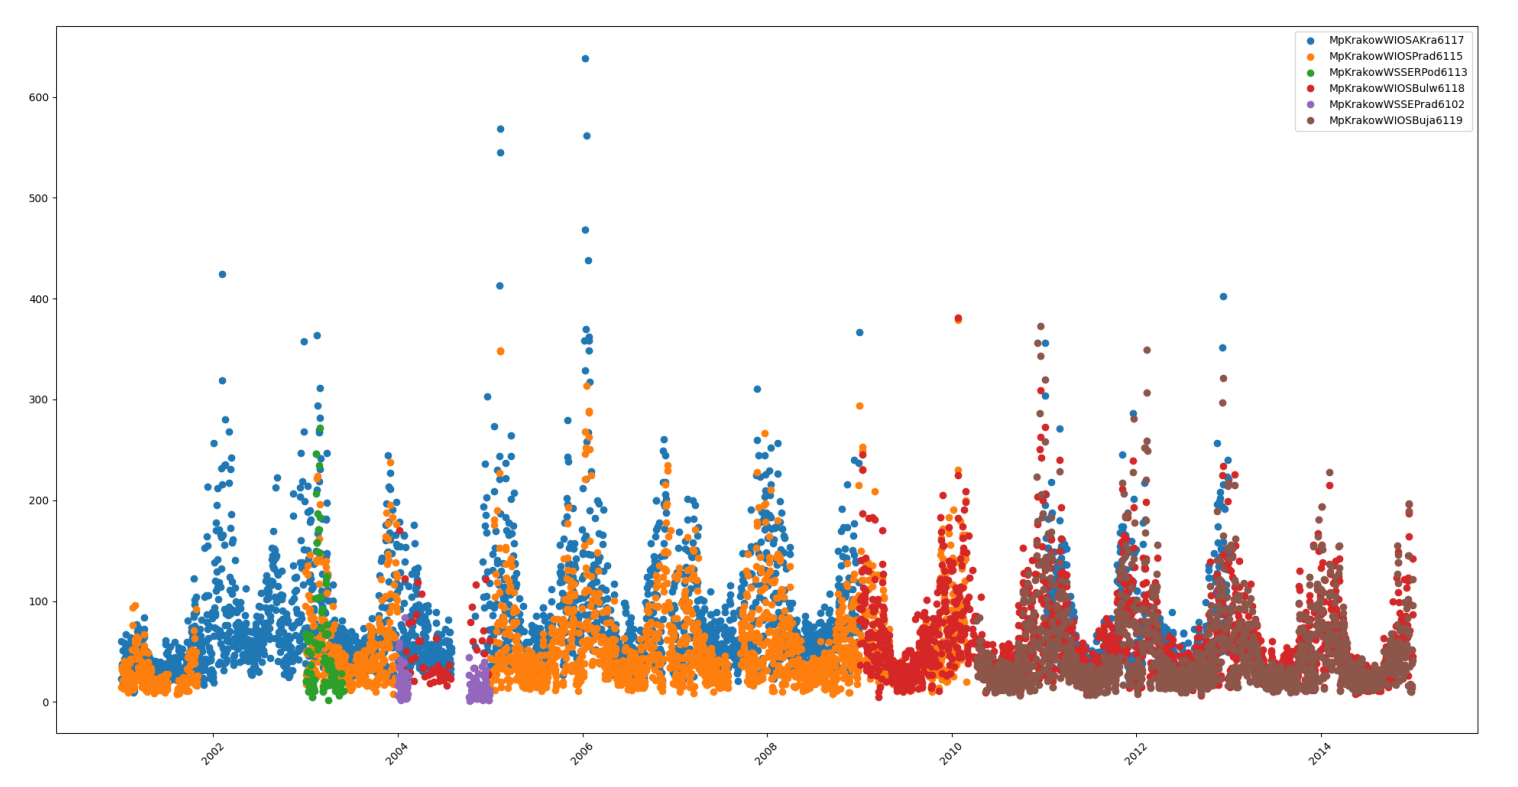
\includegraphics[scale=0.3]{gios_description_krakow.png}}
	\caption{Poziom zanieczyszczenia powietrza pyłem PM10 w Krakowie w latach 2001-2020}
	\label{figure:gios}
\end{figure}
\FloatBarrier

\subsection{Tworzenie szeregów z obu źródeł danych}
Podjęta została decyzja o połączeniu obu źródeł danych w jeden szereg czasowy. Celem tego działania było umożliwienie predykcji stężenia pyłu PM10 na podstawie danych klimatycznych. Szereg taki jest badawczo ciekawy oraz zdaje się odpowiadać stanom rzeczywistym.

Różnice w położeniu sieci stacji pomiarowych Instytutu Meteorologii i Gospodarki Wodnej oraz Głównego Inspektoratu Ochrony Środowiska stanowiły poważny problem przy próbie połączenia ich w jeden spójny szereg czasowy. Brak uwzględnienia tego ograniczenia doprowadziłby do całkowitego braku sensownego kontekstu geograficznego w otrzymanym szeregu czasowego. Problem ten został rozwiązany poprzez przygotowywanie osobnych szeregów czasowych dla wybranych stacji Instytutu i Inspektoratu o podobnym położeniu geograficznym. Sposób tworzenia takiego szeregu zostanie przedstawiony na podstawie Krakowa, następnie przedyskutowany zostanie problem tworzenia większej ilości takich szeregów. 

\subsubsection{Tworzenie szeregu dla Krakowa}
Stacja pomiarowa Instytutu Meteorologii i Gospodarki Wodnej w Krakowie posiada jedną stację pomiarową w Krakowie, której wyniki zostały ujęte w danych klimatycznych wykorzystywanych w tej pracy. Natomiast Główny Inspektorat Ochrony Środowiska w okresie będącym tematem zainteresowania tej pracy, posiadał wiele różnych punktów pomiarowych na terenie miasta. Punkty te często pojawiały się w środku okresu 2000-2020, zmieniały swoje położenie, przestawały prowadzić pomiary lub robiły przerwę w rejestrowaniu zanieczyszczeń na kilka lat. Z tego powodu nie można było skorzystać z wyników każdej ze stacji pomiarowych Instytutu jako podstawy do budowania szeregu czasowego bez jego niepotrzebnego skrócenia lub przerw utrudniających analizę. Dodatkowo ponieważ stacje GIOŚ znajdowały się w różnych częściach Krakowa, zestawianie ich z jedynym punktem pomiarowym IMGW prowadziłoby do szeregu niekoniecznie poprawnie osadzonego geograficznie. Warto również zauważyć, że niektóre stacje pomiarowe zanieczyszczenia powietrza były w obszarach z dużą ilością ruchu samochodowego, inne natomiast w obszarach ze zdecydowanie mniejszym poziomem ruchu samochodowego w okolicy. Takie rozłożenie punktów pomiarowych mogłoby sprawić, że szereg powstały na podstawie danych z jedynej stacji IMGW i jednej stacji GIOŚ mógłby być niepoprawny. Jego niepoprawność łatwo zrozumieć na przykładzie, w którym do predykcji zanieczyszczenia nad bardzo ruchliwą ulicą korzystamy jedynie z danych klimatycznych z całkowicie innej części miasta. Taka predykcja najpewniej byłaby w stanie wychwycić pewne trendy (np. ludzie częściej korzystający z samochodów w zimie), lecz nie byłyby to kompletne dane potrzebne do wiarygodnej predykcji. Pomijałoby to również wahania warunków pogodowych w różnych częściach miasta, które również mogą wpływać na zanieczyszczenie powietrza.

Aby rozwiązać powyższe problemy stworzony został szereg oparty na danych klimatycznych dostarczanych przez Instytut Meteorologii i Gospodarki Wodnej dla Krakowa oraz średnią arytmetyczną stężenia pyłu PM10 rejestrowanego przez punkty pomiarowe Głównego Inspektoratu Ochrony Środowiska znajdujące się w Krakowie. Takie podejście pozwoliło na stworzenie badawczo interesującego szeregu czasowego, który operował na średnich wartościach zanieczyszczeń w całym Krakowie bez przerw w pomiarach lub błędów. 
Operowanie na średnich wartościach zanieczyszczeń ma również dodatkową zaletę w postaci eliminacji potrzeby uwzględniania dokładnych powodów, dla których poziom zanieczyszczeń możne się różnić w poszczególnych miejscach. Takie powody to między innymi: 
\begin{itemize}
	\item Poziom przewietrzania badanego obszaru (dostępność odpowiednich korytarzy powietrznych dla kierunku wiatru w danym dniu, wysokość zabudowy itd.)
	\item Poziom ruchu ulicznego w badanym obszarze (płynność ruchu, dostępność alternatywnych form komunikacji, itd.)
	\item Sposób ogrzewania budynków (dostępność sieci ciepłowniczej, poziom zamożności społeczności lokalnej, itd.)
\end{itemize}
Powodów takich można wymienić znacznie więcej, jednak możliwość nie brania ich pod uwagę znacząco upraszcza dalsze rozważania, zwłaszcza że celem tej pracy nie jest ich dokładna analiza. Dbanie o dokładność szeregu służy tylko upewnieniu się, że przeprowadzane predykcje nie odbiegają znacząco od stanu faktycznego. 
\newpage

\subsubsection{Skalowalność predykcji}
Przy badaniu przydatności rekurencyjnych sieci neuronowych do predykcji czasowych należy skupić się również na potrzebie skalowalności uzyskanych modeli predykcyjnych. Nie ma żadnej gwarancji, że model predykcyjny uzyskujący zadowalające wyniki dla małych zbiorów danych utrzyma zadowalający poziom dokładności predykcji dla zdecydowanie większych zbiorów danych. Z tego powodu niezbędne jest stworzenie większej liczby zróżnicowanych geograficznie szeregów w celu lepszego zrozumienia użyteczności badanych modeli. 

W tym celu zbudowane zostały szeregi czasowe dla każdej odpowiadającej sobie geograficznie i czasowo pary punktów pomiarowych z Instytutu Meteorologii i Gospodarki Wodnej oraz Głównego Inspektoratu Ochrony Środowiska. W przypadkach, gdzie występowały wiele punktów mierzących stężenie pyłu PM10 przeprowadzano uśrednianie wyników pomiarów analogicznie do przypadku krakowskiego. Mniejsza uwaga została również poświęcona potrzebie ciągłości szeregu, jako że braki w pewnym fragmencie czasu były ,,przykrywane'' przez inne szeregi. Korzystając z takiej metodologii sporządzone zostały szeregi dla wszystkich sensownych par punktów pomiarowych obu instytucji.

\newpage
\section{Przeprowadzone badania}
W celu zbadania przydatności rekurencyjnych sieci neuronowych do predykcji szeregów czasowych zestawione ze sobą zostały jakości wyników różnych modeli predykcyjnych. Analizowano zarówno klasyczne metody predykcyjne jak i nowocześniejsze wykorzystujące sieci neuronowe. Celem takiego porównywania było wyłonienie najbardziej obiecującego badawczo modelu predykcyjnego w celu dalszej analizy jego wydajności. Dalsza analiza jego wydajności polegała na zbadaniu zmian zachowania modelu przy zwiększającej się ilości danych. 

W tym rozdziale przedstawiona zostanie metodologia obu etapów analizy przydatności rekurencyjnych sieci neuronowych do predykcji szeregów czasowych. 
\subsection{Porównanie wydajności modeli predykcyjnych}
Pierwszym stadium analizy było zbadanie różnych metod predykcji szeregów czasowych na przykładzie prostego szeregu czasowego. W tym etapie analizy jako zbiór danych wykorzystywany jest szereg zbudowany dla Krakowa, opisany w rozdziale \hyperlink{subsubsection.3.3.1}{3.3.1}. Celem tego procesu jest porównanie jakości wyników zwracanych przez modele oparte na rekurencyjnych sieciach neuronowych z klasycznymi metodami predykcji. Poszukiwany jest również najlepszy model rekurencyjny mogący zostać wykorzystany w dalszych badaniach. 

\subsubsection{Regresja liniowa}
Pierwszą metodą zastosowaną do predykcji była regresja liniowa, jako że jest ona jedną z najstarszych i dobrze przebadanych metod predykcyjnych. Jej wyniki pełniły w dalszych rozważaniach rolę grupy kontrolnej dla wyników uzyskiwanych przez inne metody.

Regresja liniowa została przeprowadzona korzystając z metod udostępnionych w ramach biblioteki ,,sklearn'' dla języka Python. Biblioteka ta daje możliwość przeprowadzenia prostej regresji liniowej metodą najmniejszych kwadratów \cite{sklearnLinearRegression}.

W celu poprawnego podziału danych na zbiór uczący i testujący wykorzystana została metoda ,,train\_test\_split'' z tej samej biblioteki ,,sklearn''. Zdefiniowano tej metodzie, że 20\% danych powinno stanowić zbiór testujący, a pozostałe dane powinny być użyte do uczenia modelu. 

W celu umożliwienia ewaluacji wyników działania metody, sporządzony został wykres zestawiający przewidziane wartości z wynikami pomiarów oraz wyliczone zostało kilka charakterystyk pozwalających na porównanie. Charakterystyki te to:
\begin{center}
	\begin{itemize}
		\item Wynik testu $R^2$
		\item Błąd średniokwadratowy
		\item Pierwiastek błędu średniokwadratowego
		\item Wartość indeksu Willmott'a
	\end{itemize}
\end{center}

Uzyskane w tej metodzie wyniki zostaną dokładnie przedyskutowane w podsekcji \hyperlink{subsubsection.5.1.1}{5.1.1} oraz zestawione z wynikami pozostałych metod w podsekcji \hyperlink{subsubsection.5.1.6}{5.1.6}.

\subsubsection{Drzewa decyzyjne}
Drugą zastosowaną metodą była regresja z wykorzystaniem drzew decyzyjnych, jako że jest ona jedną z najszerzej wykorzystywanych metod uczenia maszynowego. Podobnie jak w przypadku regresji liniowej, uzyskane wyniki pełnią funkcję grupy kontrolnej. Warty odnotowania jest również fakt użyteczności graficznych reprezentacji procesu decyzyjnego do zrozumienia nie tylko sposobu podejmowania decyzji, ale również struktury danych wejściowych. 

Regresja z wykorzystaniem drzew decyzyjnych została przeprowadzona za pomocą metod udostępnionych w bibliotece ,,sklearn'' dla języka Python. Biblioteka ta definiuje drzewa decyzyjne jako nieparametryczną metodę nadzorowanego uczenia używaną do klasyfikacji i regresji \cite{sklearnDecissionTrees}. Aspekt regresyjny został wykorzystany w prowadzonych badaniach. 

Zastosowany został podział na zbiór uczący i testujący analogicznie jak w przypadku regresji liniowej. Tak samo analogiczne podejście zostało przyjęte w liczeniu charakterystyk porównawczych wyników. Więcej szczegółów podziału i wyliczanych charakterystyk można znaleźć w podsekcji \hyperlink{subsubsection.4.1.1}{4.1.1}.

Dla ułatwienia zrozumienia otrzymywanych wyników sporządzony został również rysunek ostatecznego drzewa decyzyjnego. Rysunek ten został wykonany korzystając z języka opisu grafów DOT \cite{dotLanguage}.

Wyniki regresji z wykorzystaniem drzew decyzyjnych zostaną dokładnie przedstawione w podsekcji \hyperlink{5.1.2}{5.1.2} oraz porównane z wynikami innych metod w podsekcji \hyperlink{5.1.6}{5.1.6}.

\subsubsection{Sieci rekurencyjne}
W ramach badania przydatności rekurencyjnych sieci neuronowych do badania szeregów czasowych rozważane były trzy rodzaje architektury sieci neuronowej. Badano zachowanie prostej rekurencyjnej sieci neuronowej, sieci typu LSTM oraz GRU. Uzyskane w ten sposób wyniki zostaną przeanalizowane w kontekście przydatności tej metody oraz w kontekście jej wydajności w porównaniu do nowocześniejszych architektur sieci rekurencyjnych. 

Sieć neuronowa posiadała również proste warstwy wejściowe i wyjściowe wymagane do poprawnej pracy warstw ukrytych z wykorzystywanym w badaniach zbiorem danych.
Dla każdej rozważanej architektury tworzona była oparta na niej warstwa ukryta, dostarczana w ramach biblioteki ,,TensorFlow'' dla języka Python. Dla prostej sieci rekurencyjnej była to ,,SimpleRNN'' \cite{tfSimpleRNN}, dla sieci Long Short-Term Memory  warstwa ,,LSTM'' \cite{tfLSTM}, a dla sieci Gated Recurrent Unit warstwa ,,GRU'' \cite{tfGRU}.

Zastosowany został podział na zbiór uczący i testujący analogicznie jak w przypadku regresji liniowej. Tak samo analogiczne podejście zostało przyjęte w liczeniu charakterystyk porównawczych wyników. Więcej szczegółów podziału i wyliczanych charakterystyk można znaleźć w podsekcji \hyperlink{subsubsection.4.1.1}{4.1.1}.
Badany był również wpływ liczby neuronów w warstwie ukrytej na jakość uzyskiwanych wyników. 

Wyniki predykcji zostaną dokładnie przedstawione w podsekcjach odpowiadających każdej w zastosowanych architektur oraz porównane z wynikami innych metod w podsekcji \hyperlink{5.1.6}{5.1.6}.


\subsection{Badanie skalowalności modelu GRU}
Jak zauważono poprzednio, skalowalność modelu ma duże znaczenie przy określaniu jego przydatności do predykcji szeregów czasowych. W celu zbadania skalowalności modelu opartego na architekturze Gated Recurrent Unit przeprowadzono serię uczenia i testowania dla szeregów czasowych o zwiększającej się liczbie elementów. 

Sieć neuronowa posiadała analogiczną budowę do sieci GRU opisanej w podsekcji \hyperlink{subsubsection.4.1.3}{4.1.3}. Wymagane były zmiany w warstwie wejściowej umożliwiające współpracę z różnymi wymiarami danych wejściowych.

W ramach badania przeprowadzone zostało łącznie dwadzieścia dziewięć procesów uczenia i walidacji stworzonego modelu. W każdym kolejnym kroku badania do wejściowego szeregu czasowego dodawany był nowy szereg czasowy dla położenia geograficznego nie ujętego w poprzednich danych. 

Przeprowadzone zostały identyczne pomiary wydajności modelu oraz wizualne zestawienia wyników predykcji z danymi rzeczywistymi. Sporządzony został również wykres wartości indeksu Willmott'a dla każdego przeprowadzonego procesu uczenia i walidacji modelu.

Przyjęcie takiej metodologii badania skalowalności pozwala wierzyć, że otrzymane wyniki będą pomocne w określeniu przydatności tejże sieci do predykcji szeregów czasowych. Wyniki te zostaną przedstawione w podsekcji \hyperlink{subsection.5.2}{5.2}.

\newpage
\section{Numeryczna analiza zagadnienia predykcji koncentracji PM10}
W ramach tego rozdziału przedstawione zostaną wyniki wszystkich przeprowadzonych badań. Zostanie również przeprowadzona analiza wyników każdej metody z osobna oraz analiza porównawcza wyników wielu metod. Celem tej analizy jest zapewnienie pełnego kontekstu niezbędnego do wyciągania wniosków, które zostaną omówione w kolejnym rozdziale. 

\subsection{Porównanie wydajności modeli predykcyjnych}
W tym podrozdziale poświęcona zostanie szczególna uwaga wynikom uzyskiwanym przez poszczególne modele, problemom występującym w procesie badawczym oraz zestawieniu wyników wszystkich metod. Oczekuje się, że opis wyników oraz ich analiza przedstawią wystarczający poziom dokładności pozwalający przenieść uwagę na wyciąganie wniosków.
 
\subsubsection{Regresja liniowa}
W procesie badania efektywności regresji liniowej do predykcji szeregu czasowego uzyskane zostały parametry opisujące poprawność predykcji oraz wizualne zestawienie wartości przewidywanych i realnych. W tej podsekcji zostaną one przedstawione oraz omówione. 

W pierwszej kolejności opisane zostaną uzyskane wartości parametrów określające poprawność wyników. Wyliczone zostały parametry:
\begin{center}
	\begin{itemize}
		\item wynik testu ($R^2$)
		\item błąd średniokwadratowy (MSE)
		\item pierwiastek błędu średniokwadratowego (RMSE)
		\item indeks Willmott'a
	\end{itemize}
\end{center}
Wartości powyższych parametrów zostały przedstawione w \autoref{table:1}. Zostaną one wykorzystane w celu porównania jakości uzyskiwanych wyników z innymi metodami.
\begin{table}[h!]
	\centering
	\begin{tabular}{|c|c|c|c|}
		\hline
		$R^2$ & MSE & RMSE & Willmott \\
		\hline
		0,32 & 1386,29 & 37,23 & 0,672 \\
		\hline
	\end{tabular}
		\caption{Wartości opisujące poprawność wyników regresji liniowej}
		\label{table:1}
\end{table}

Na \autoref{figure:linear} przedstawione zostało zestawienie wyników uzyskanych przez regresję liniową z wynikami obserwacji. Wyniki będące rezultatem regresji są na rysunku zaznaczone kolorem pomarańczowym, a pierwotny szereg czasowy kolorem niebieskim. Na osi x znajdują się daty z przedziału [01.01.2000 - 31.12.2020], na osi y natomiast poziom stężenia pyłu PM10 w $\frac{\si{\micro\gram}}{\si\meter^3}$. 

Wykres ten pokazuje, że regresja metodą najmniejszych kwadratów dobrze przystosowała się do okresowości badanego szeregu. Poprawnie ukazała zmiany zanieczyszczenia w różnych porach roku. Wychwyciła również ogólny trend zmniejszającego się poziomu zanieczyszczeń w kolejnych latach. Można również zaobserwować, że regresja liniowa napotkała trudności w przewidywaniu bardzo wysokich poziomów zanieczyszczeń w zimie. 

\begin{figure}[!ht]
	\centering
	\makebox[0pt]{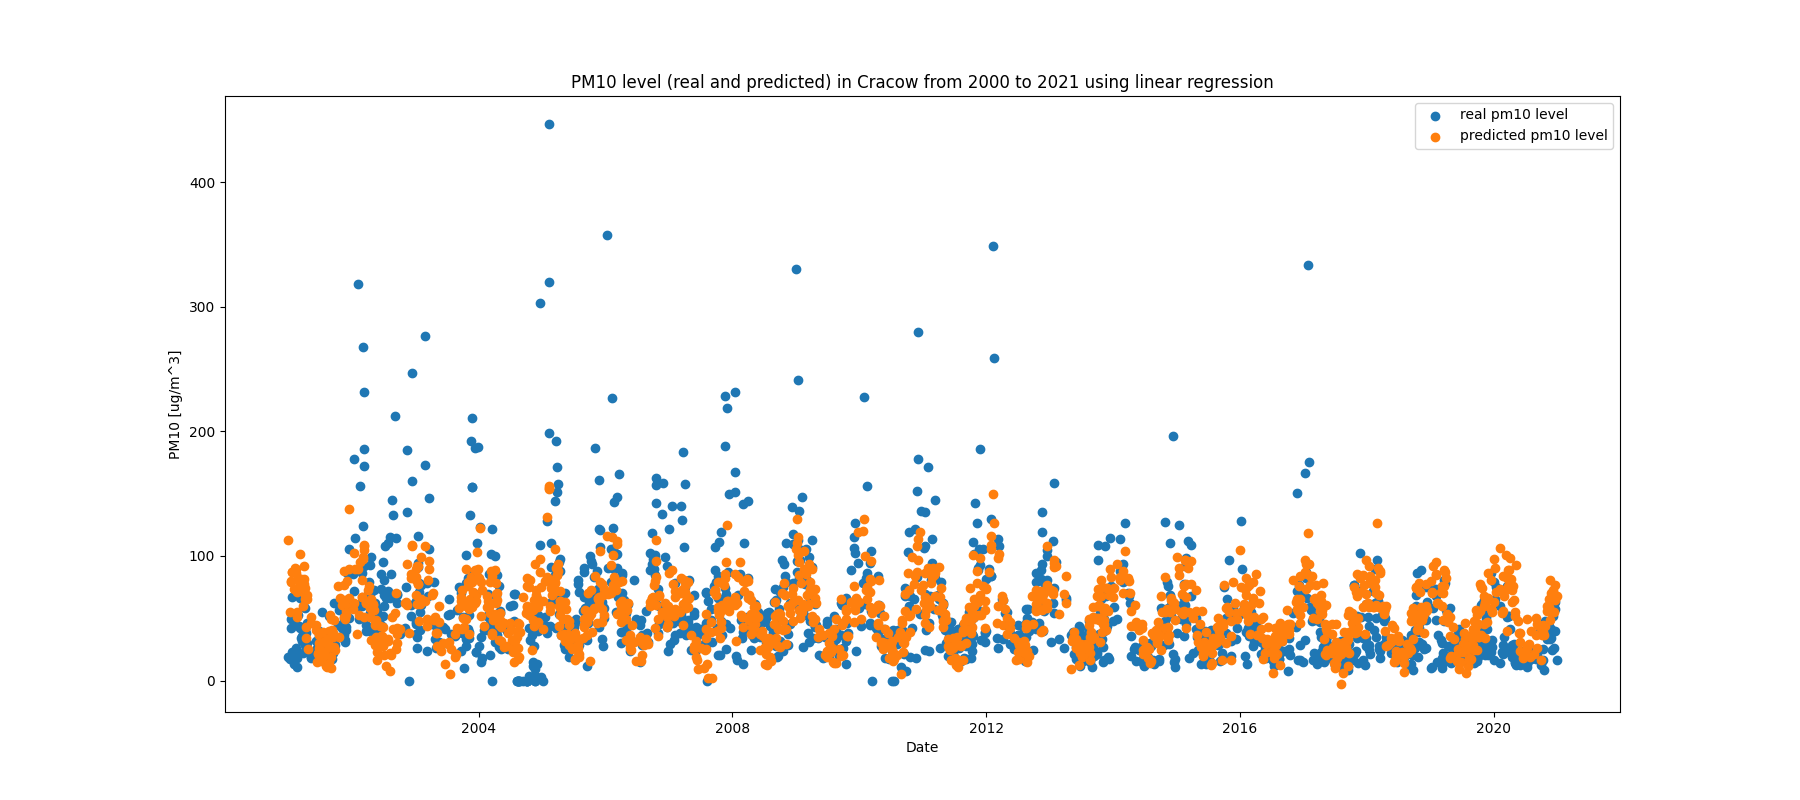
\includegraphics[scale=0.4]{linear.png}}
	\caption{Zestawienie wyników regresji liniowej z prawdziwymi obserwacjami}
	\label{figure:linear}
\end{figure}
\FloatBarrier
\subsubsection{Drzewa decyzyjne}
Podczas badania efektywności drzew decyzyjnych do predykcji szeregów czasowych stworzone zostały zostały parametry opisujące jakość wyników, zestawienie predykcji z danymi pomiarowymi oraz wizualizacja drzewa decyzyjnego. Stworzono również zestawienie jakości wyników predykcji w zależności od dozwolonej głębokości drzewa. 

W \autoref{table:2} przedstawione zostały wyniki parametrów opisujących jakość otrzymanych predykcji. Przedstawione w tabeli są:
\begin{center}
	\begin{itemize}
		\item wynik testu ($R^2$)
		\item błąd średniokwadratowy (MSE)
		\item pierwiastek błędu średniokwadratowego (RMSE)
		\item indeks Willmott'a
	\end{itemize}
\end{center}
Warto zauważyć, że o ile wartość indeksu Willmott'a utrzymuje się na podobnym poziomie to pozostałe parametry zmieniają się znacząco wraz ze wzrostem głębokości drzewa. Szczególnie interesującym wskaźnikiem jest wynik testu $R^2$, który spada w szybkim tempie i osiąga wartości ujemne. Zazwyczaj ujemne wartości tego testu oznaczają, że sposób predykcji nie jest odpowiedni dla danych wejściowych. Zmiana ta została zaprezentowana na \autoref{figure:treer2}, gdzie na osi X prezentowana jest głębokość drzewa, a na osi Y wynik testu $R^2$. Na tej podstawie wyznaczona została optymalna głębokość drzewa dla analizowanego problemu. Wartości parametrów dla tej konfiguracji zostały wytłuszczone w \autoref{table:2}.

\begin{table}[h!]
	\centering
	\begin{tabular}{|c|c|c|c|c|}
		\hline
		Głębokość drzewa & $R^2$ & MSE & RMSE & Willmott \\
		\hline
		3  & 0,31  & 1409,99 & 37,55 & 0,671 \\
		4  & 0,33  & 1376,81 & 37,11 & 0,688 \\
		\textbf{5}  & \textbf{0,28}  & \textbf{1476,42} & \textbf{38,42} & \textbf{0,685} \\
		6  & 0,25  & 1530,27 & 39,12 & 0,685 \\
		7  & 0,20  & 1637,53 & 40,47 & 0,683 \\
		8  & 0,13  & 1786,99 & 42,27 & 0,672 \\
		9  & 0,05  & 1939,26 & 44,04 & 0,661 \\
		10 & -0,01 & 2055,84 & 45,34 & 0,645 \\
		11 & -0,12 & 2288,05 & 47,83 & 0,610 \\
		12 & -0,13 & 2320,77 & 48,17 & 0,612 \\
		13 & -0,19 & 2430,74 & 49,30 & 0,610 \\
		14 & -0,28 & 2623,67 & 51,22 & 0,601 \\
		\hline
	\end{tabular}
	\caption{Parametry opisujące poprawność wyników regresji liniowej}
	\label{table:2}
\end{table}
\begin{figure}[!ht]
	\centering
	\makebox[0pt]{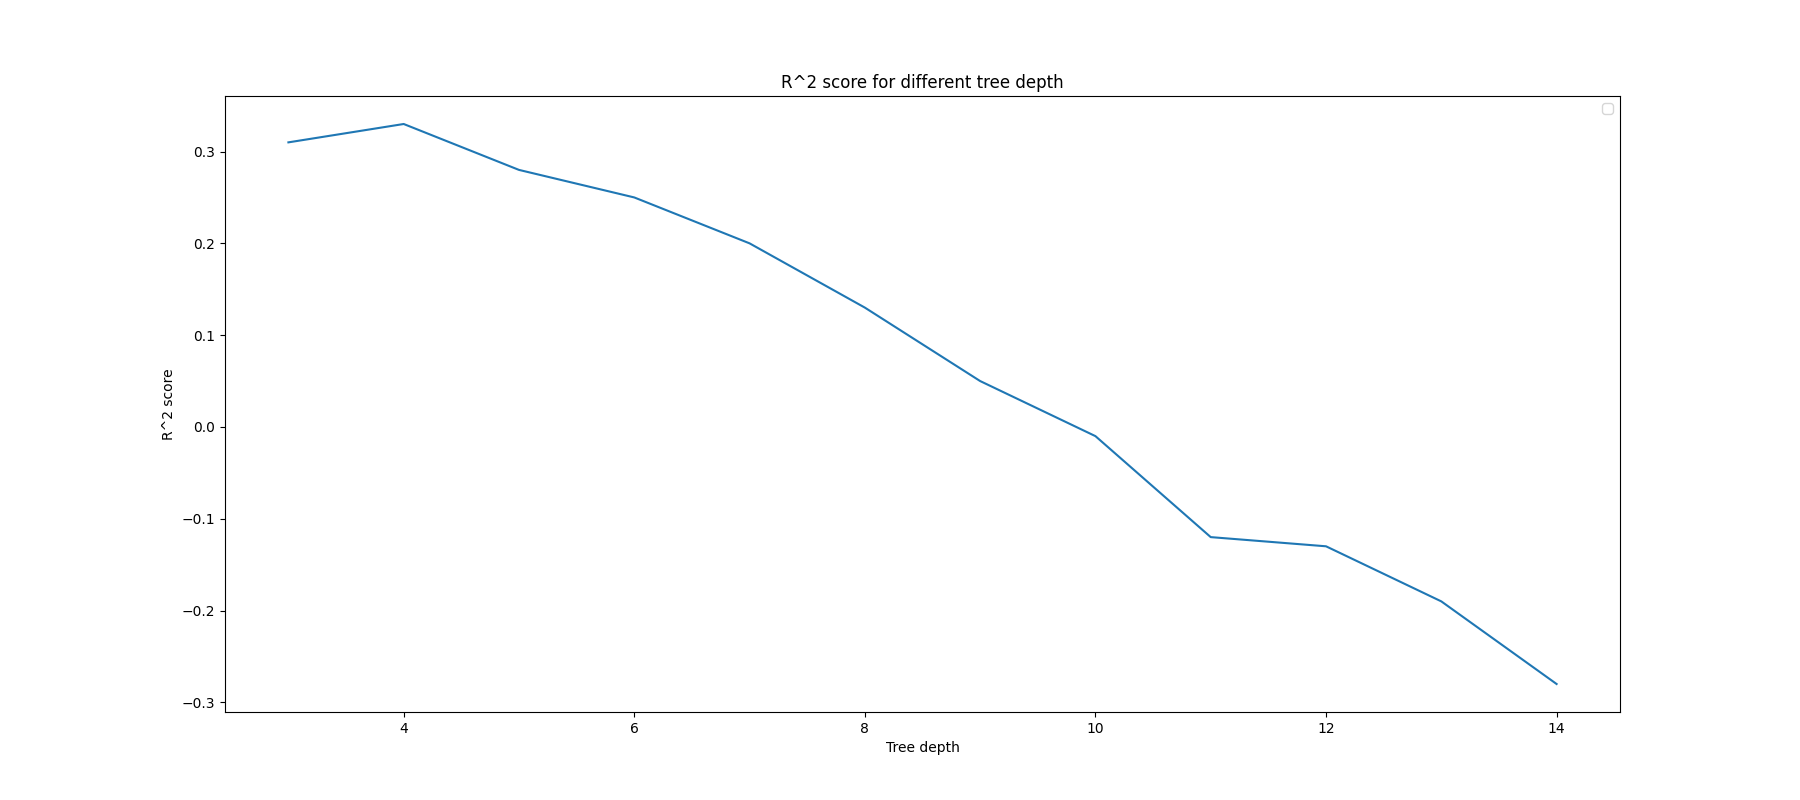
\includegraphics[scale=0.42]{trees_r2.png}}
	\caption{Zmiana wyniku testu $R^2$ dla różnych głębokości drzewa}
	\label{figure:treer2}
\end{figure}
\FloatBarrier
\begin{figure}[!ht]
	\centering
	\makebox[0pt]{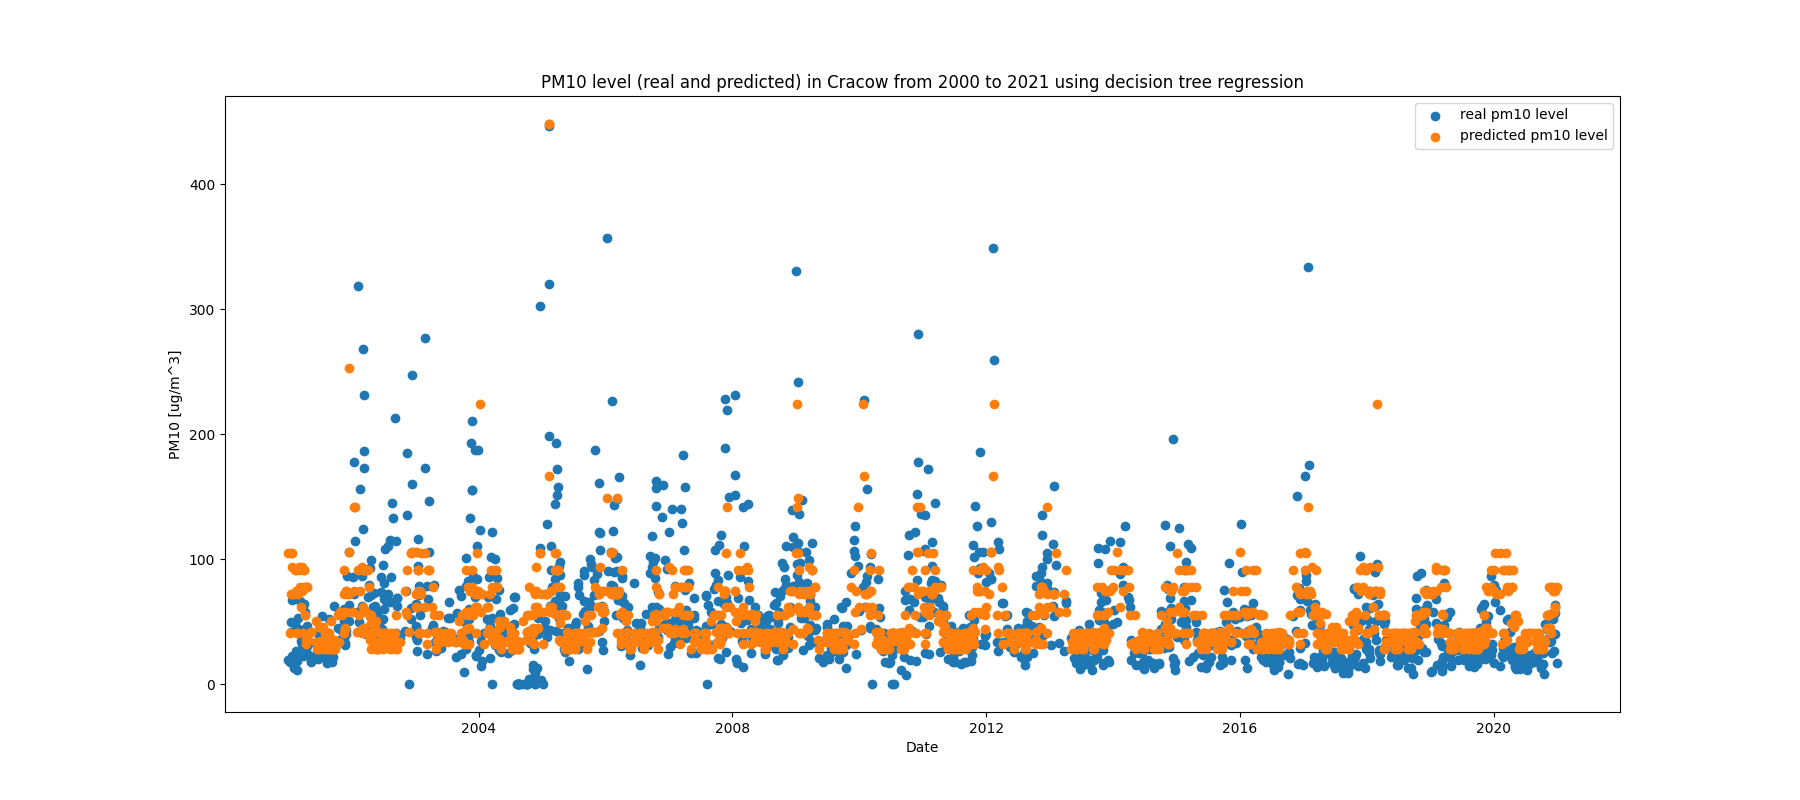
\includegraphics[scale=0.4]{decission_tree_5.png}}
	\caption{Zestawienie wyników drzewa o głębokości 5 z prawdziwymi obserwacjami}
	\label{figure:tree5}
\end{figure}
\FloatBarrier
\begin{figure}[!ht]
	\centering
	\makebox[0pt]{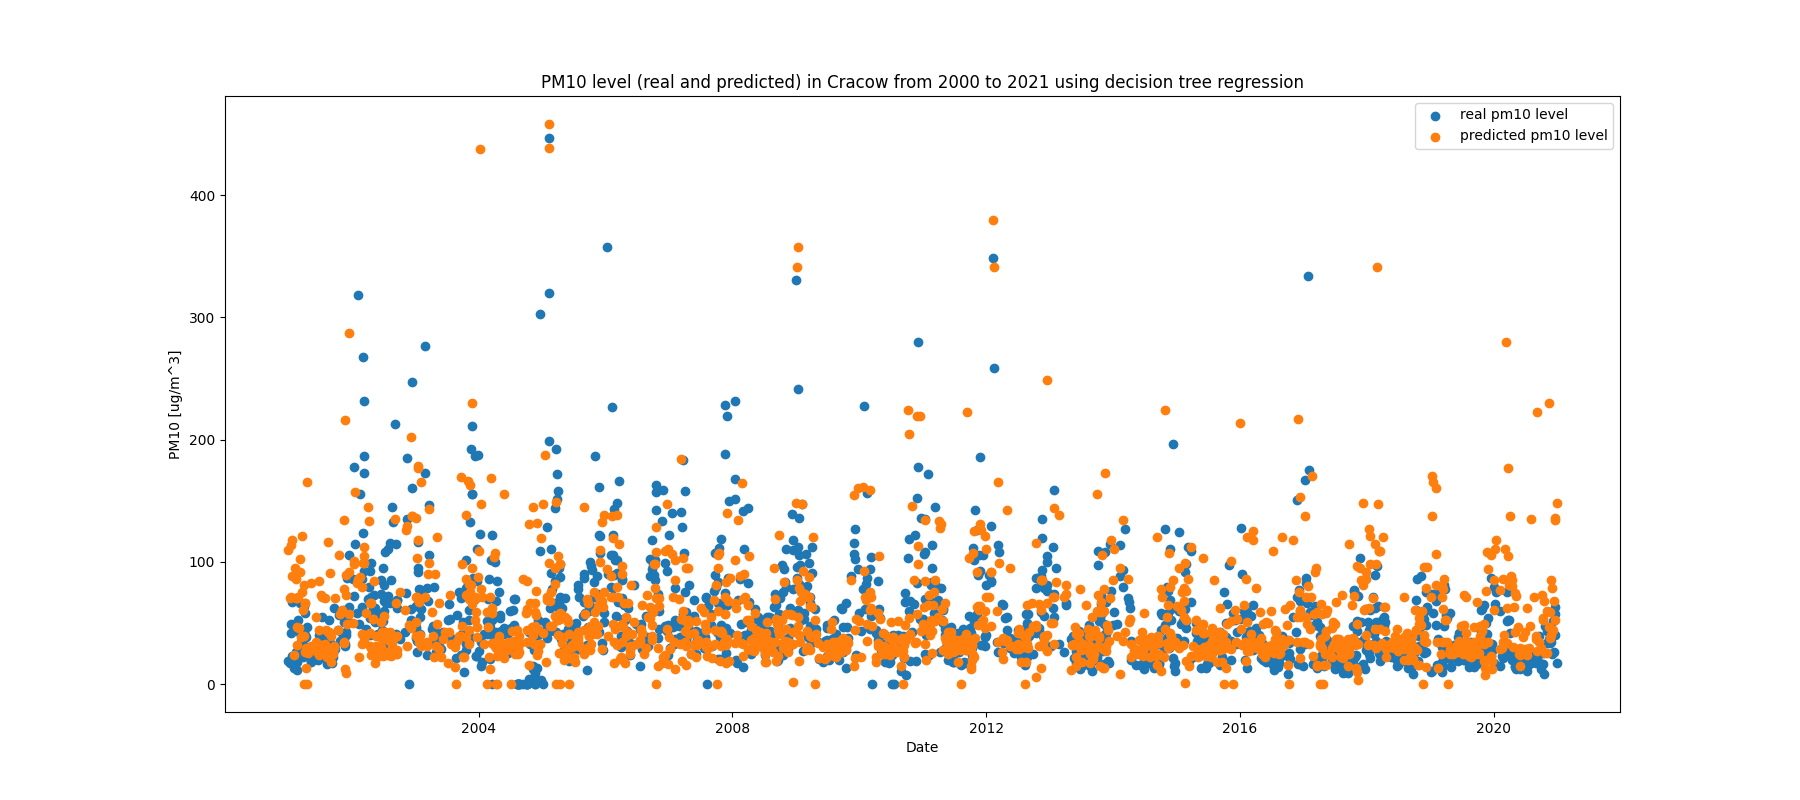
\includegraphics[scale=0.4]{decission_tree_14.png}}
	\caption{Zestawienie wyników drzewa o głębokości 14 z prawdziwymi obserwacjami}
	\label{figure:tree14}
\end{figure}
\FloatBarrier

Na \autoref{figure:tree5} i \autoref{figure:tree14} przedstawione są wyniki predykcji w zestawieniu z pierwotnymi obserwacjami w szeregu. Na \autoref{figure:tree5} z powodu ograniczonej wielkości drzewa, większość przypadków decyzyjnych znajduje się w przedziale (0 - 100) $\frac{\si{\micro\gram}}{\si\meter^3}$ co pozwala na relatywnie poprawne odwzorowanie zbioru danych. Natomiast na \autoref{figure:tree14} z powodu większej głębokości drzewa tworzone są przypadki decyzyjne dla bardzo odosobnionych, bardzo wysokich wartości zanieczyszczeń, które nie reprezentują większości danych wejściowych. 

Z tego powodu przyjęte zostało założenie wykorzystywania optymalnej głębokości drzewa w dalszej analizie porównawczej z innymi modelami. Nieuczciwy byłby wybór takiego drzewa decyzyjnego, w którym poprzez zbyt dużą głębokość drzewa wyniki predykcji nie odwzorowują adekwatnie danych wejściowych, jeżeli zmiana głębokości pozwala na otrzymanie wierniejszych oryginałowi predykcji.

Sporządzona została również wizualizacja procesu decyzyjnego dla drzewa o głębokości równej pięć, pozwalająca lepiej zrozumieć działanie drzewa decyzyjnego. Jest ona przedstawiona na \autoref{figure:tree_graph} i pozwala zauważyć wyraźnie drzewiastą strukturę procesu podejmowania decyzji. Nie jest niestety możliwe zawarcie tej ilustracji w wystarczająco dużym formacie, aby móc przyjrzeć się dokładnie poszczególnym liściom drzewa. Z tego powodu stworzona została również wizualizacja dla drzewa o głębokości równej 3 przedstawiona na \autoref{figure:tree_graph_small}

\begin{figure}[!ht]
	\centering
	\makebox[0pt]{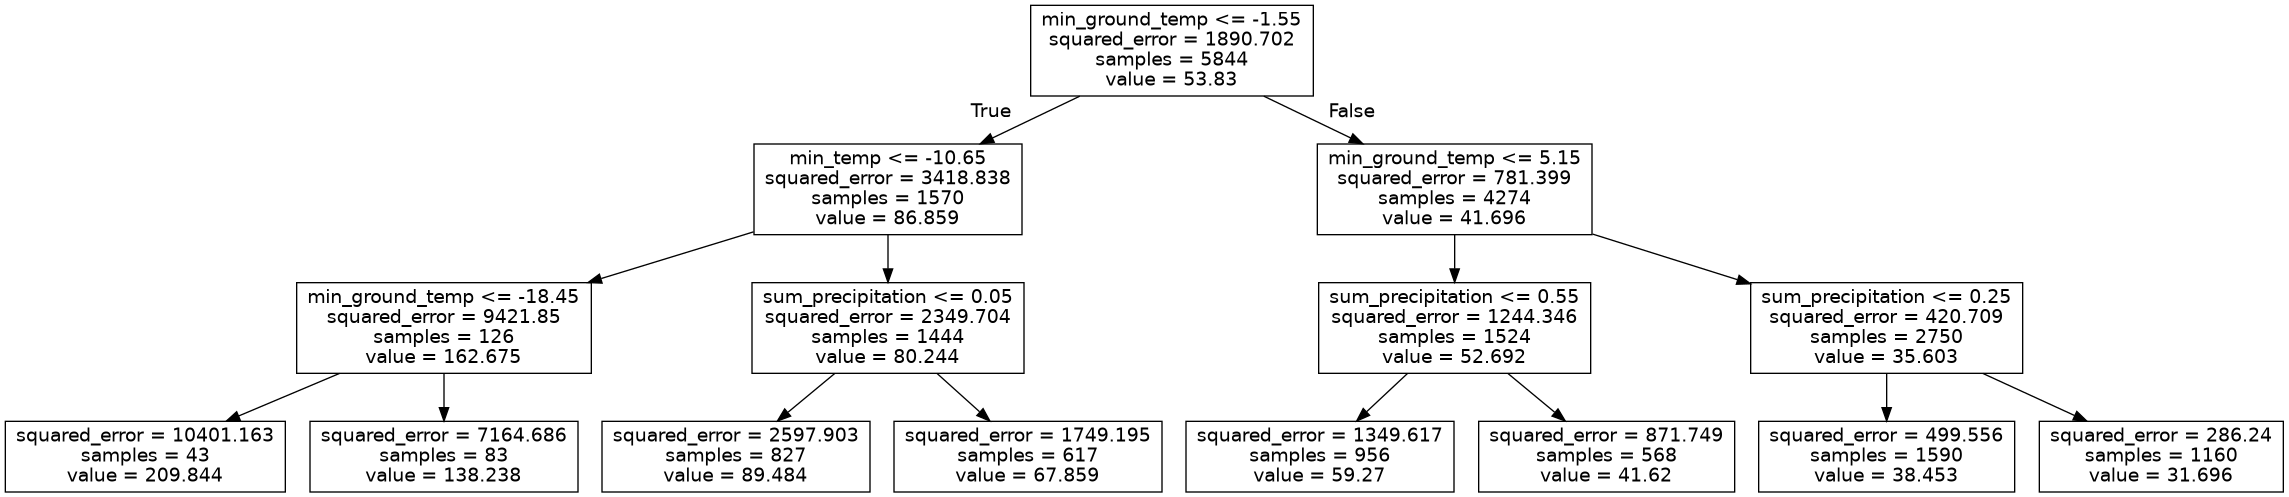
\includegraphics[scale=0.25]{tree.png}}
	\caption{Proces decyzyjny drzewa o głębokości równej 3}
	\label{figure:tree_graph_small}
\end{figure}
\FloatBarrier

\begin{figure}[!ht]
	\centering
	\makebox[0pt]{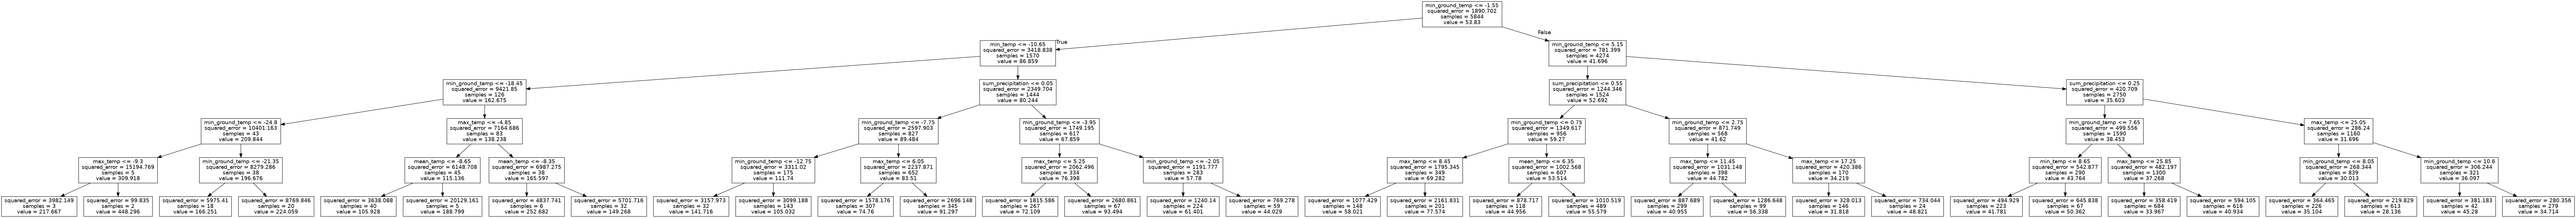
\includegraphics[scale=0.064,angle=90]{decission_tree_tree.png}}
	\caption{Proces decyzyjny drzewa o głębokości równej 5}
	\label{figure:tree_graph}
\end{figure}
\FloatBarrier
Taka wizualizacja pozwala na lepsze zrozumienie zbioru danych i znaczenia różnych parametrów klimatycznych obecnych w szeregu czasowym. Za pierwszy punkt podziału oba drzewa przyjmują fakt występowania przymrozku w danym dniu. Dalsza analiza pozwala zaobserwować inne ciekawe sytuacje bezpośrednio wpływające na poziom zanieczyszczeń. Na przykład zarówno w lewej jak i prawej części drzewa, fakt występowania opadu atmosferycznego implikuje zwiększony poziom zanieczyszczeń. 

\subsubsection{Prosta sieć rekurencyjna}
W ramach badania przydatności prostej sieci rekurencyjnej uzyskane zostały wartości parametrów opisujących jakość wyników modelu oraz graficzne reprezentacje rozwiązania dostarczanego przez model. Wyniki te zostaną przedstawione i przedyskutowane w ramach tej podsekcji.


W \autoref{table:simpleRNN} przedstawione zostały wyniki parametrów opisujących jakość otrzymanych predykcji. Przedstawione w tabeli są:
\begin{center}
	\begin{itemize}
		\item wynik testu ($R^2$)
		\item błąd średniokwadratowy (MSE)
		\item pierwiastek błędu średniokwadratowego (RMSE)
		\item indeks Willmott'a
	\end{itemize}
\end{center}

Korzystając z tych danych można zaobserwować, że wartości parametrów poprawiają się wraz ze wzrostem liczby neuronów. Takie zjawisko nie powinno być w żadnym wypadku zaskakujące, można spodziewać się, że większa sieć będzie lepiej przetwarzać dane wejściowe. Warto jednak zauważyć, że nie występuje liniowa zależność pomiędzy wzrostem ilości neuronów oraz dokładnością predykcji. Mając na uwadze ten fakt oraz znaczące zwiększenie się czasu uczenia większych sieci, warto postarać się o znalezienie optymalnej liczby neuronów w warstwie ukrytej. Potencjalnie optymalne konfiguracje liczby neuronów została wytłuszczona na \autoref{table:simpleRNN}. Zależność ta została przedstawiona na \autoref{figure:simple_rnn_neurons}.

\begin{table}[h!]
	\centering
	\begin{tabular}{|c|c|c|c|c|}
		\hline
		Liczba neuronów w warstwie ukrytej & $R^2$ & MSE & RMSE & Willmott \\
		\hline
		1    & -0,63 & 3347,90 & 57,86 & 0,396 \\
		2    & -0,37 & 2798,97 & 52,91 & 0,374 \\
		4    & -0,05 & 2155,29 & 46,43 & 0,305 \\
		8    & 0,15  & 1734,83 & 41,65 & 0,419 \\
		16   & 0,24  & 1546,97 & 39,33 & 0,575 \\
		32   & 0,31  & 1418,95 & 37,67 & 0,646 \\
		64   & 0,35  & 1334,45 & 36,53 & 0,690 \\
		\textbf{128}  & \textbf{0,38}  & \textbf{1277,33} & \textbf{35,74} & \textbf{0,711} \\
		\textbf{256}  & \textbf{0,39}  & \textbf{1256,35} & \textbf{35,45} & \textbf{0,719} \\
		512  & 0,38  & 1267,64 & 35,60 & 0,725 \\
		1024 & 0,38  & 1270,25 & 35,64 & 0,700 \\
		\hline
	\end{tabular}
	\caption{Parametry opisujące poprawność wyników predykcji prostej sieci neuronowej}
	\label{table:simpleRNN}
\end{table}
\begin{figure}[!ht]
	\centering
	\makebox[0pt]{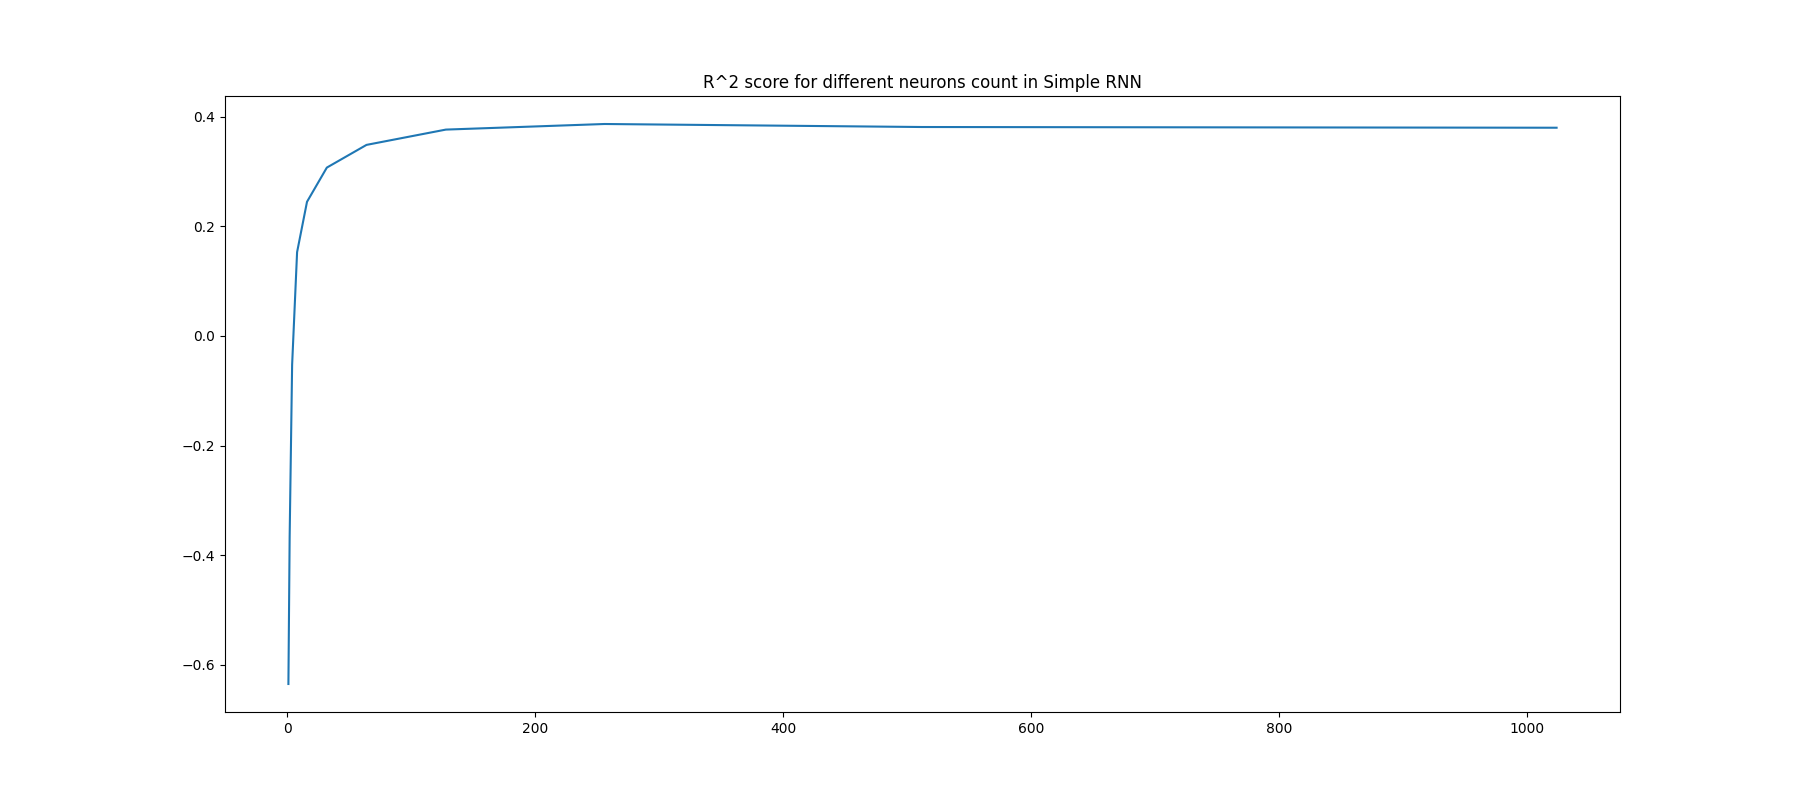
\includegraphics[scale=0.3]{simple_rnn_neurons.png}}
	\caption{Wynik testu $R^2$ dla różnej liczby neuronów w warstwie ukrytej}
	\label{figure:simple_rnn_neurons}
\end{figure}
\FloatBarrier
 \begin{figure}[!ht]
	\centering
	\makebox[0pt]{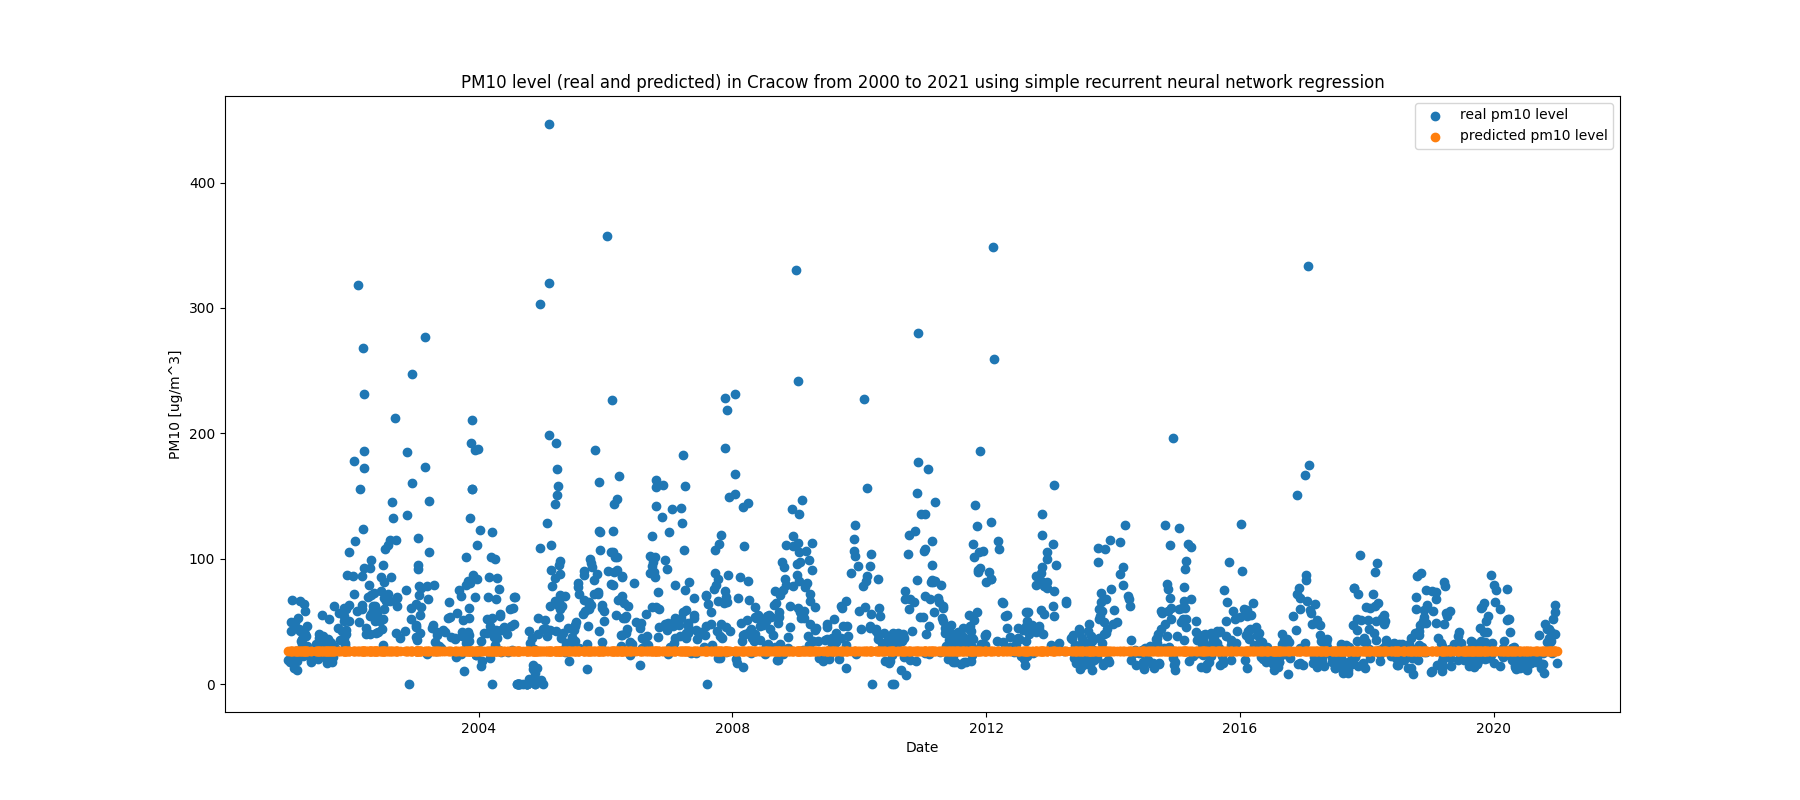
\includegraphics[scale=0.4]{simpleRNN_2.png}}
	\caption{Zestawienie wyników prostej rekurencyjnej sieci neuronowej z dwoma neuronami w warstwie ukrytej z prawdziwymi obserwacjami}
	\label{figure:simple_rnn_2}
\end{figure}
\FloatBarrier
 \begin{figure}[!ht]
	\centering
	\makebox[0pt]{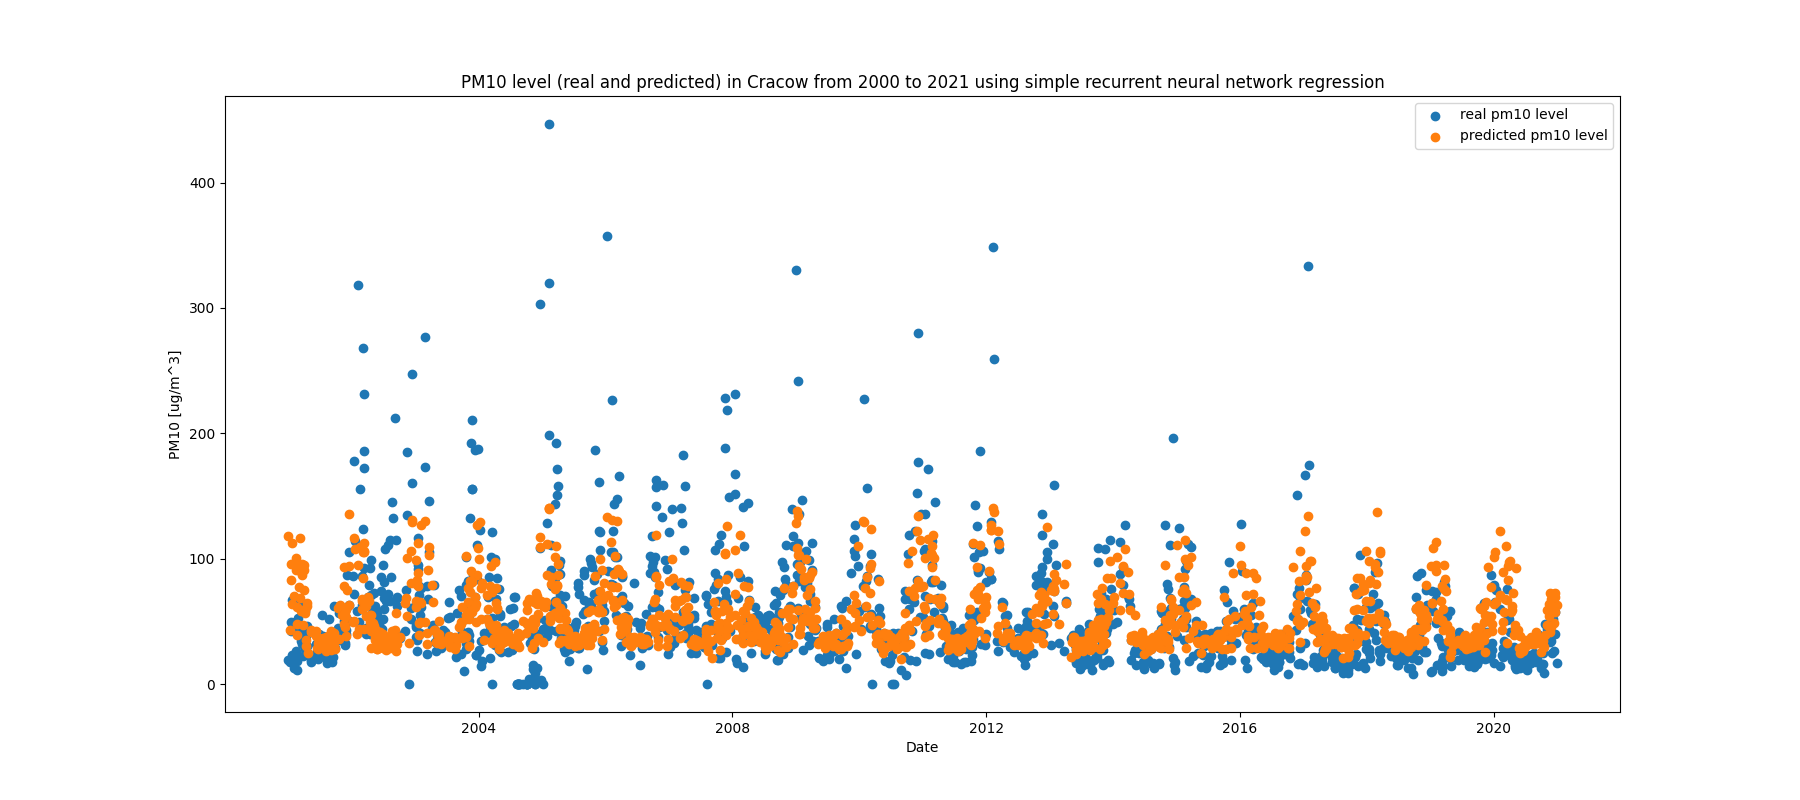
\includegraphics[scale=0.4]{simpleRNN_64.png}}
	\caption{Zestawienie wyników prostej rekurencyjnej sieci neuronowej z 64 neuronami w warstwie ukrytej z prawdziwymi obserwacjami}
	\label{figure:simple_rnn_64}
\end{figure}
\FloatBarrier
 \begin{figure}[!ht]
	\centering
	\makebox[0pt]{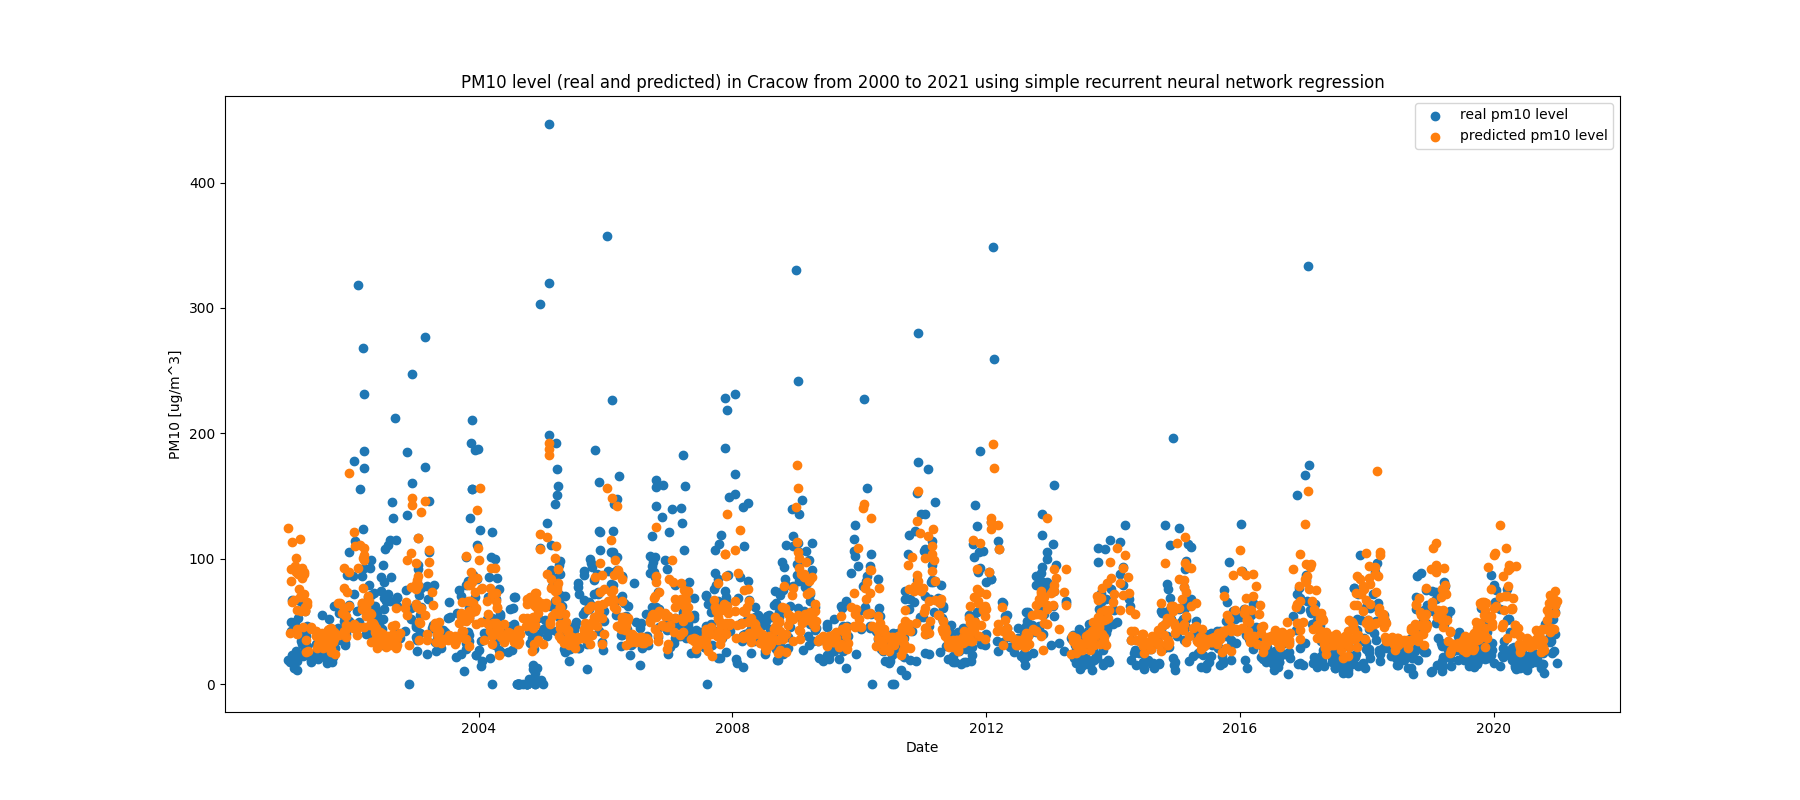
\includegraphics[scale=0.4]{simpleRNN_512.png}}
	\caption{Zestawienie wyników prostej rekurencyjnej sieci neuronowej z 512 neuronami w warstwie ukrytej z prawdziwymi obserwacjami}
	\label{figure:simple_rnn_512}
\end{figure}
\FloatBarrier

Na \autoref{figure:simple_rnn_2}, \autoref{figure:simple_rnn_64}, \autoref{figure:simple_rnn_512} przedstawione zostały zestawienia wyników predykcji z danymi zgromadzonymi w pierwotnym szeregu czasowym. Bliższa analiza tych rysunków pozwoli lepiej zrozumieć wpływ liczby neuronów w warstwie ukrytej na jakość otrzymywanych predykcji. Na \autoref{figure:simple_rnn_2} można zaobserwować zachowanie sieci neuronowej, która nie posiada wystarczającej liczby neuronów. Model taki nie odwzorowuje poprawnie danych wejściowych, ponieważ jest zdecydowanie zbyt prosty do przedstawiania jakkolwiek sensownych predykcji. 

Ciekawsze są dwa kolejne rysunki przedstawiające 64 i 512 neuronów w warstwie ukrytej. Można zaobserwować, że te modele odwzorowują dane wejściowe ze zdecydowanie wyższą precyzją. Warto zwrócić uwagę na fakt, że różnice pomiędzy tymi dwoma modelami nie są dramatyczne i na pewno nie proporcjonalne do różnicy w liczbie neuronów. Interesujący może być fakt, że przy zwiększeniu liczby neuronów sieć stara się bardziej dopasowywać do bardzo wysokich poziomów zanieczyszczeń. To zachowanie może implikować występowanie problemu zbytniego dopasowywania się do danych wejściowych, które było widoczne w zbyt głębokich drzewach decyzyjnych.

Ostatecznie warto zauważyć, że niezależnie od liczby neuronów w warstwie ukrytej, sieci mają problem z wychwyceniem długotrwałego trendu zmniejszenia się poziomu zanieczyszczeń w kolejnych latach. Dobrze rozumieją one okresowość danych wejściowych, ale zdają się nie mieć wystarczającej liczby informacji do wychwycenia trendu. 
\newpage
\subsubsection{Sieć rekurencyjna typu LSTM}
W ramach badania przydatności sieci rekurencyjnej opartej na architekturze Long Short-Term Memory zebrane zostały wyniki analogicznie jak przy badaniu prostej sieci rekurencyjnej. W tym podrozdziale zostaną one przedstawione oraz przeanalizowane w izolacji od innych metod predykcyjnych. 

W \autoref{table:lstm} przedstawione zostały wartości parametrów opisujących dokładność wyników predykcji w zależności od liczby neuronów w warstwie ukrytej. Są to takie same parametry jak w pozostałych metodach, więc nie zostaną one tutaj dokładniej przedstawione. Na podstawie danych w tabeli możemy zaobserwować wyraźną poprawę parametrów wraz ze wzrostem liczby neuronów w warstwie ukrytej. Relacja ta została zaprezentowana na \autoref{figure:lstm_neurons} i jest bardzo wyraźnie nieliniowa. Na podstawie analizy tej relacji w \autoref{table:lstm} wyróżnione zostały wyniki sieci z potencjalnie optymalnymi wielkościami warstwy ukrytej.

\begin{table}[h!]
	\centering
	\begin{tabular}{|c|c|c|c|c|}
		\hline
		Liczba neuronów w warstwie ukrytej & $R^2$ & MSE & RMSE & Willmott \\
		\hline
		1    & -0,68 & 3445,70 & 58,70 & 0,398 \\
		2    & -0,49 & 3045,89 & 55,19 & 0,387 \\
		4    & -0,16 & 2375,20 & 48,74 & 0,317 \\
		8    & 0,10  & 1850,13 & 43,01 & 0,300 \\
		16   & 0,21  & 1613,10 & 40,16 & 0,508 \\
		32   & 0,30  & 1425,17 & 37,75 & 0,635 \\
		64   & 0,34  & 1341,85 & 36,63 & 0,680 \\
		128  & 0,38  & 1276,60 & 35,73 & 0,699 \\
		256  & 0,39  & 1239,25 & 35,20 & 0,715 \\
		512  & 0,41  & 1217,06 & 34,89 & 0,734 \\
		1024 & 0,41  & 1217,79 & 34,90 & 0,748 \\
		\hline
	\end{tabular}
	\caption{Parametry opisujące poprawność wyników sieci LSTM}
	\label{table:lstm}
\end{table}
\begin{figure}[!ht]
	\centering
	\makebox[0pt]{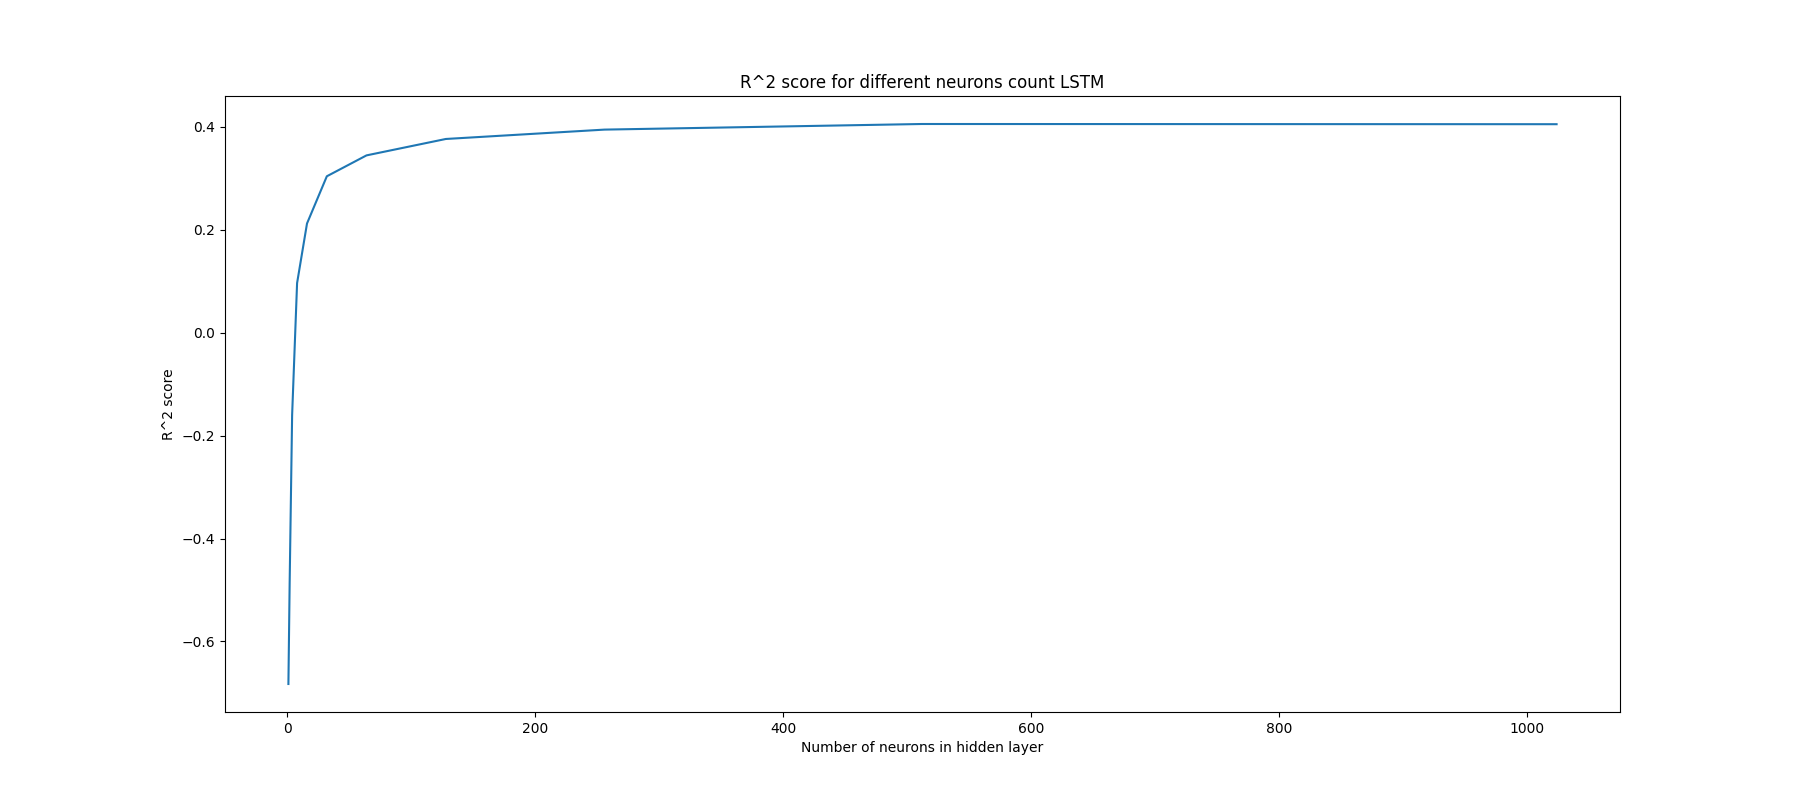
\includegraphics[scale=0.3]{lstm_neurons.png}}
	\caption{Wynik testu $R^2$ dla różnej liczby neuronów w warstwie ukrytej}
	\label{figure:lstm_neurons}
\end{figure}
\FloatBarrier
\begin{figure}[!ht]
	\centering
	\makebox[0pt]{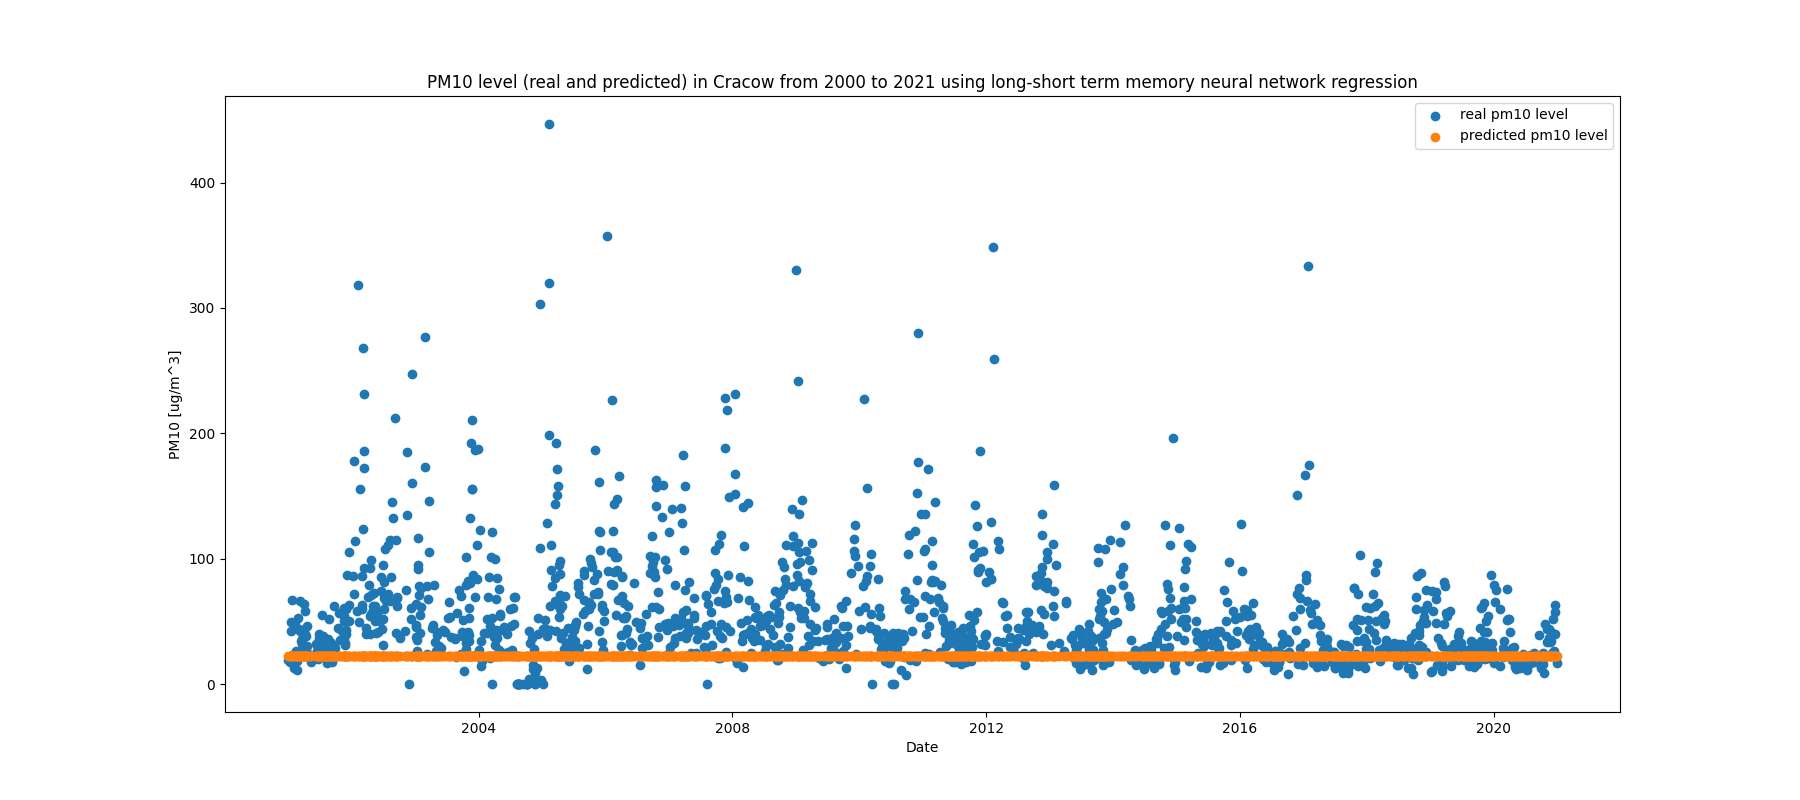
\includegraphics[scale=0.4]{LSTM_2.png}}
	\caption{Zestawienie wyników sieci LSTM z dwoma neuronami w warstwie ukrytej z prawdziwymi obserwacjami}
	\label{figure:lstm_2}
\end{figure}
\FloatBarrier
\begin{figure}[!ht]
	\centering
	\makebox[0pt]{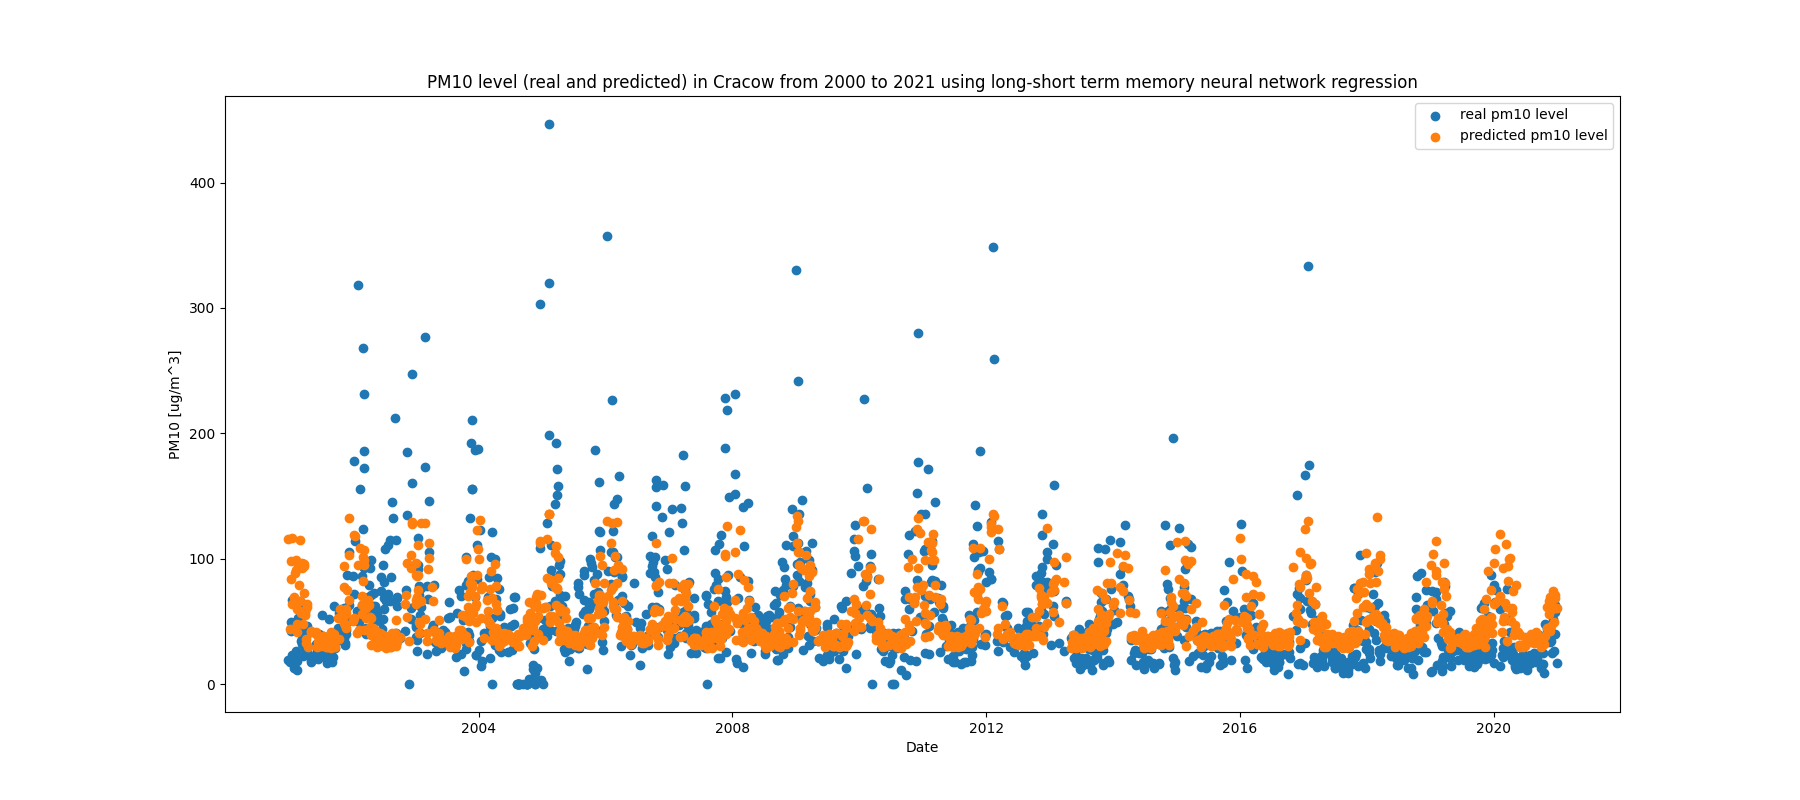
\includegraphics[scale=0.4]{LSTM_64.png}}
	\caption{Zestawienie wyników sieci LSTM z 64 neuronami w warstwie ukrytej z prawdziwymi obserwacjami}
	\label{figure:lstm_64}
\end{figure}
\FloatBarrier
\begin{figure}[!ht]
	\centering
	\makebox[0pt]{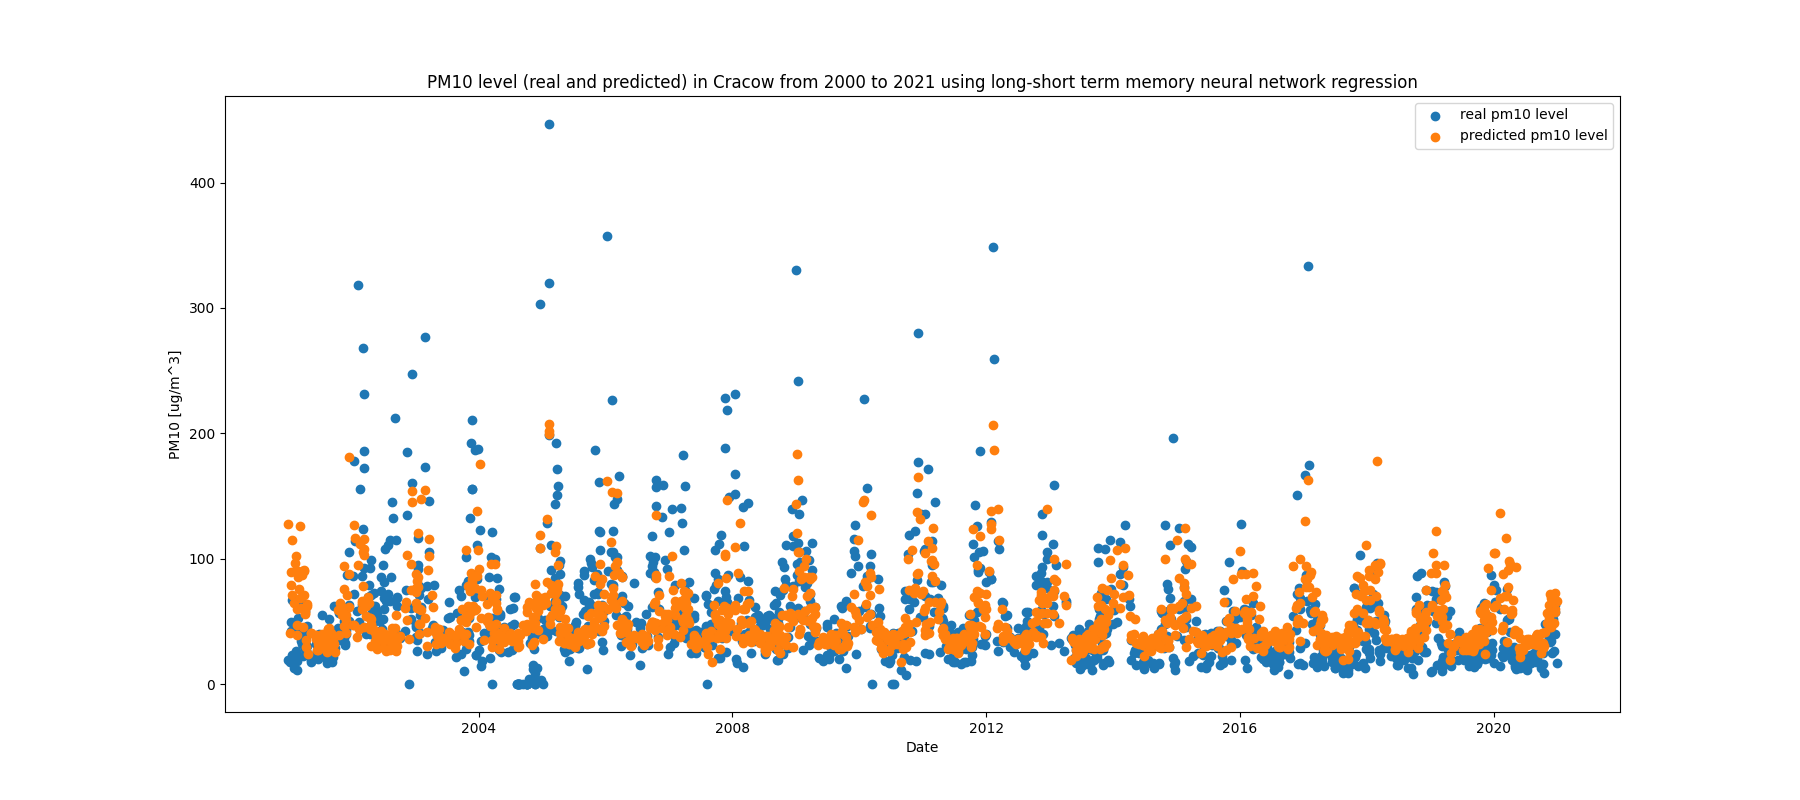
\includegraphics[scale=0.4]{LSTM_512.png}}
	\caption{Zestawienie wyników sieci LSTM z 512 neuronami w warstwie ukrytej z prawdziwymi obserwacjami}
	\label{figure:lstm_512}
\end{figure}
\FloatBarrier

Na \autoref{figure:lstm_2}, \autoref{figure:lstm_64} oraz \autoref{figure:lstm_512} przedstawione zostały zestawienia predykcji sieci neuronowej typu LSTM z danymi obserwacyjnymi. Prezentowany jest realny i przewidziany poziom zanieczyszczenia pyłem PM10 w perspektywie czasowej. Na osi x reprezentowany jest czas w dniach, a na osi y stężenie pyłu PM10 w  $\frac{\si{\micro\gram}}{\si\meter^3}$. Rysunki te odzwierciedlają wyraźniej fenomen obserwowany w \autoref{table:lstm} stanowiąc użyteczny mechanizm do zrozumienia działania modelu. 

Wyraźnie odznacza się całkowity brak dopasowania modelu z dwoma neuronami w warstwie ukrytej do danych wejściowych. Tak małej sieci neuronowej brakuje mocy do poprawnego przetworzenia informacji wejściowej oraz cechuje się tendencją do nadmiernej generalizacji, przez co całkowicie mija się z danymi wejściowymi. Brakuje jej również mocy obliczeniowej potrzebnej do przystosowania się do długofalowego trendu obecnego w danych. Taki model jest zdecydowanie nieadekwatny i nie powinien być wykorzystywany w dalszych analizach. 

Natomiast zarówno modele prezentowane na \autoref{figure:lstm_64} i \autoref{figure:lstm_512} w relatywnie poprawny sposób odtwarzają dane wejściowe. Model z 512 neuronami w warstwie ukrytej zdaje się generować dokładniejsze odtworzenie zbioru wejściowego. Jednak różnica ta nie wydaje się być radykalna i na pewno nie jest proporcjonalna do zmiany liczby neuronów. Obserwacja ta umacnia wnioski płynące z \autoref{figure:lstm_neurons}, że od pewnego momentu zmiana wielkości warstwy ukrytej zaczyna mieć niewielki wpływ na jakość uzyskiwanych wyników. 

Przykładem obrazującym wyższą dokładność predykcji większego modelu może być zwiększona uwaga poświęcana bardzo wysokim poziomom zanieczyszczeń, które model z 64 neuronami w warstwie ukrytej co do zasady pomija w predykcjach. Taka próba dopasowywania do wszystkich wyników zbioru może prowadzić do niebezpieczeństw zbytniego dopasowywania do zbioru danych, podobnego do zbyt głębokiego drzewa decyzyjnego.

Niestety, niezależnie do liczności warstwy ukrytej wszystkie sieci mają problem z wychwyceniem ogólnego trendu zmniejszania się zanieczyszczeń. Zgodnie z założeniami architektury sieć typu Long Short-Term Memory powinna być w stanie poradzić sobie z takim zadaniem. Jednak trend, którego nie potrafi zauważyć żadna z sieci jest zasadniczo niewielki i może być niewystarczający dla sieci do odnotowania. 

Mając na uwadze te aspekty wpływu modelu na jakość wyników oraz zwiększony koszt obliczeniowy dla większych sieci neuronowych należy starać znaleźć optymalną wielkość sieci do predykcji danego szeregu. Aspektem ważnym do rozważenia podczas tego poszukiwania powinny być różnice w prędkości uczenia różnych sieci neuronowych.

\subsubsection{Sieć rekurencyjna typu GRU}
W ramach badania sieci Gated Recurrent Memory dane zostały zebrane analogicznie jak w innych analizowanych modelach predykcyjnych. W tym podrozdziale zostaną one przedstawione oraz przeanalizowane pod kątem wyboru optymalnych parametrów sieci do dalszej analizy. 

W \autoref{table:gru} przedstawione zostały wartości parametrów opisujące jakość wyników predykcji z wykorzystaniem sieci neuronowej w architekturze GRU. Są one ukazane w zależności od liczby neuronów w warstwie ukrytej. Prezentowane są dokładnie takie same parametry jak w innych metodach predykcyjnych. Dokładna analiza tych parametrów pozwoli na lepsze zrozumienie działania sieci opartej na architekturze Gated Recurrent Unit. 

Wyraźnie widoczna jest poprawa wartości parametrów wraz z wzrostem liczby neuronów w warstwie ukrytej. Zmiana ta nie jest jednak jednolita, istnieją nawet spadki wartości indeksu Willmott'a podczas wzrostu liczby neuronów. Zjawisko to jest najpewniej lokalną anomalią, aczkolwiek warto brać pod uwagę fakt, że zwiększenie warstwy ukrytej nie musi prowadzić do lepszego wyniku. 

Przyglądając się relacji wyniku testu $R^2$ do liczby neuronów w warstwie ukrytej wyraźnie widoczna jest nieliniowość tej relacji. Została ona zaprezentowana na \autoref{figure:gru_neurons}, gdzie na osi x przedstawiana jest liczba neuronów, a na osi y wyniku testu $R^2$. Wyraźnie widoczny jest bardzo szybki początkowy wzrost wyniku testu przy niewielkim zwiększeniu wielkości warstwy ukrytej. To tempo wzrostu gwałtownie wyhamowuje w okolicy wartości 0.4 i pozostaje relatywnie stałe pomimo zwiększania liczby neuronów. Na tej podstawie można wywnioskować, że po osiągnięciu pewnego progu wzrost liczby neuronów w warstwie ukrytej nie poprawia jakości rozwiązania prezentowanego przez sieć neuronową. 

\begin{table}[h!]
	\centering
	\begin{tabular}{|c|c|c|c|c|}
		\hline
		Liczba neuronów w warstwie ukrytej & $R^2$ & MSE & RMSE & Willmott \\
		\hline
		1    & -0.5998 & 3276.1793 & 57.2379 & 0.3945 \\
		2    & -0.3570 & 2778.8420 & 52.7147 & 0.3720 \\
		4    & -0.0395 & 2128.6287 & 46.1371 & 0.3058 \\
		8    & 0.1676  & 1704.5330 & 41.2860 & 0.4393 \\
		16   & 0.2692  & 1496.4748 & 38.6843 & 0.5966 \\
		32   & 0.3341  & 1363.7161 & 36.9285 & 0.6527 \\
		64   & 0.3751  & 1279.7501 & 35.7736 & 0.7068 \\
		128  & 0.3928  & 1243.4949 & 35.2632 & 0.7207 \\
		256  & 0.3987  & 1231.2979 & 35.0899 & 0.7053 \\
		512  & 0.4057  & 1216.9403 & 34.8847 & 0.7239 \\
		1024 & 0.4048  & 1218.8890 & 34.9126 & 0.7308 \\
		\hline
	\end{tabular}
	\caption{Parametry opisujące poprawność wyników sieci GRU}
	\label{table:gru}
\end{table}
\begin{figure}[!ht]
	\centering
	\makebox[0pt]{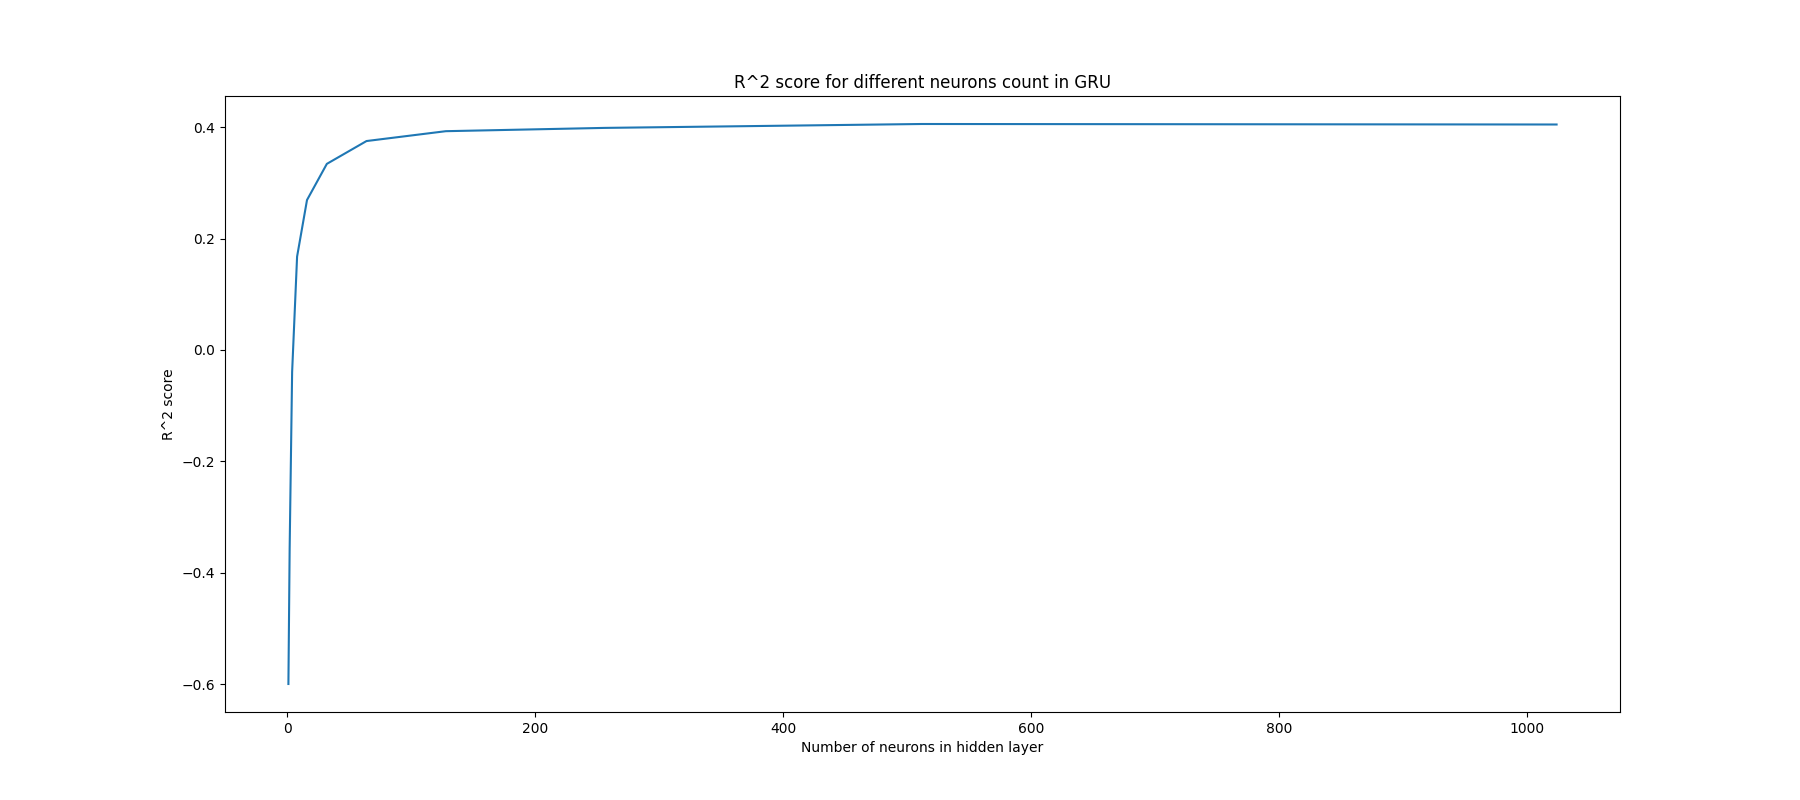
\includegraphics[scale=0.3]{gru_neurons.png}}
	\caption{Wynik testu $R^2$ dla różnej liczby neuronów w warstwie ukrytej}
	\label{figure:gru_neurons}
\end{figure}
\FloatBarrier
\begin{figure}[!ht]
	\centering
	\makebox[0pt]{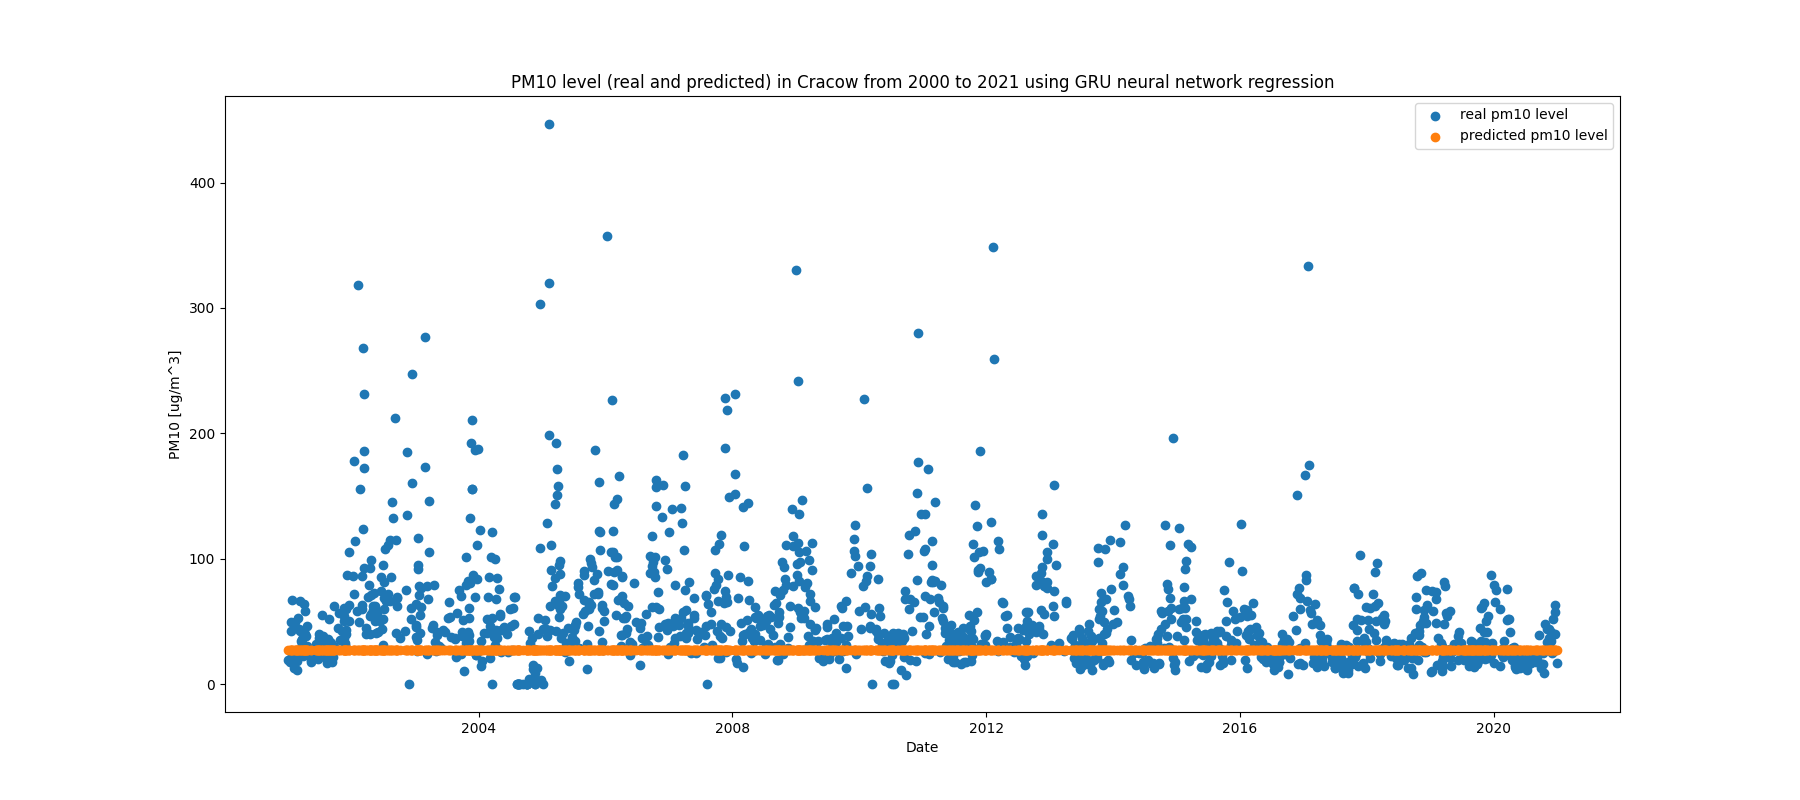
\includegraphics[scale=0.4]{GRU_2.png}}
	\caption{Zestawienie wyników sieci GRU z dwoma neuronami w warstwie ukrytej z prawdziwymi obserwacjami}
	\label{figure:gru_2}
\end{figure}
\FloatBarrier
\begin{figure}[!ht]
	\centering
	\makebox[0pt]{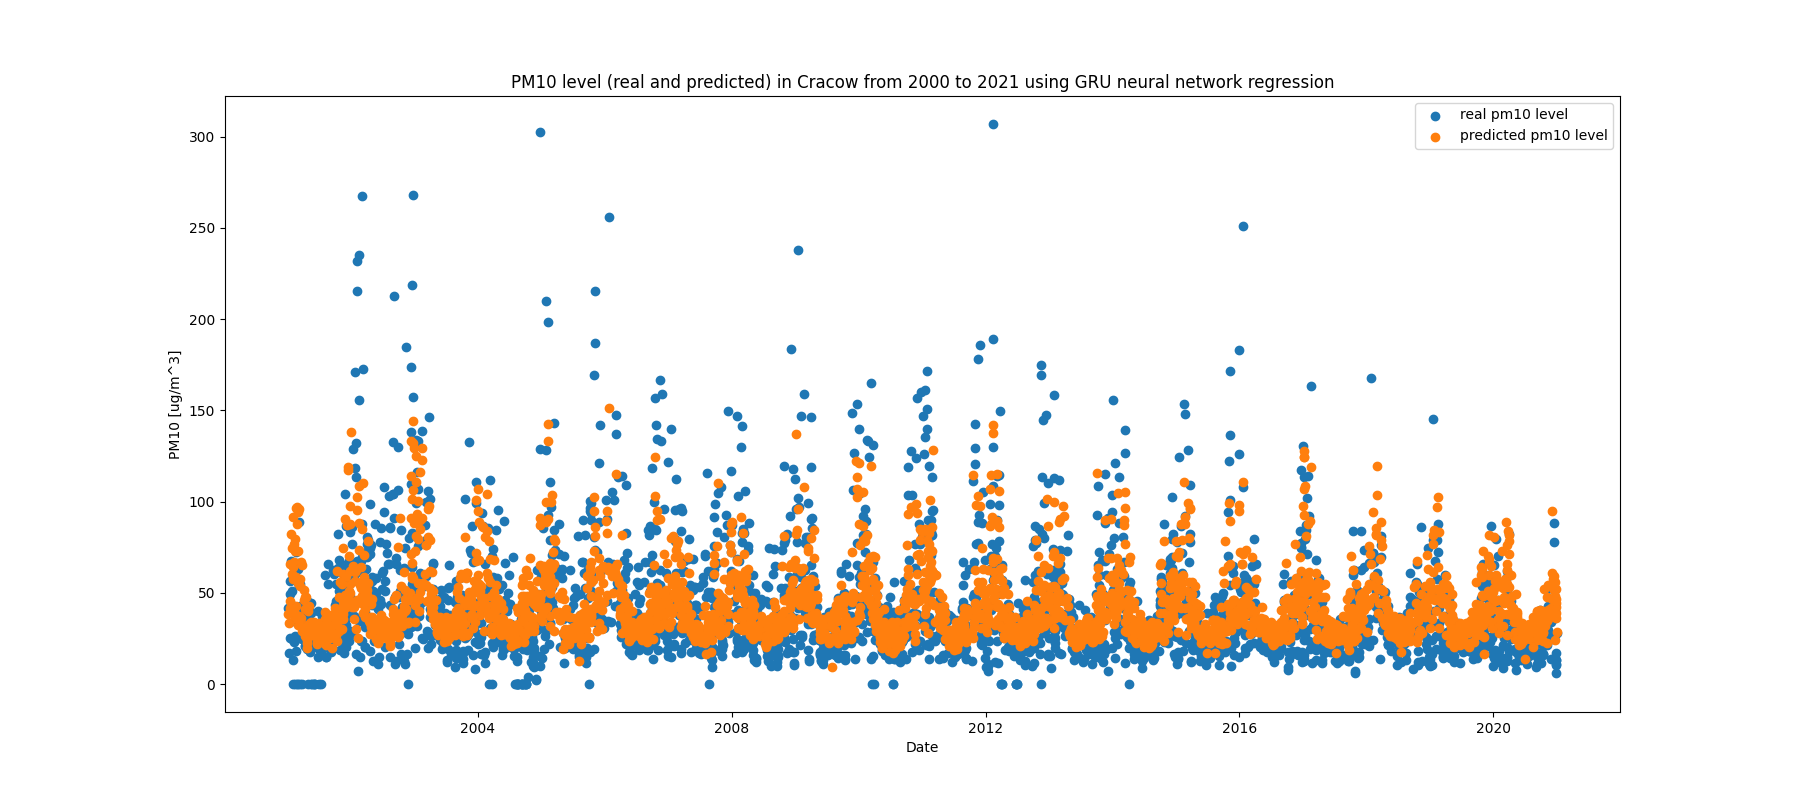
\includegraphics[scale=0.4]{GRU_64.png}}
	\caption{Zestawienie wyników sieci GRU z 64 neuronami w warstwie ukrytej z prawdziwymi obserwacjami}
	\label{figure:gru_64}
\end{figure}
\FloatBarrier
\begin{figure}[!ht]
	\centering
	\makebox[0pt]{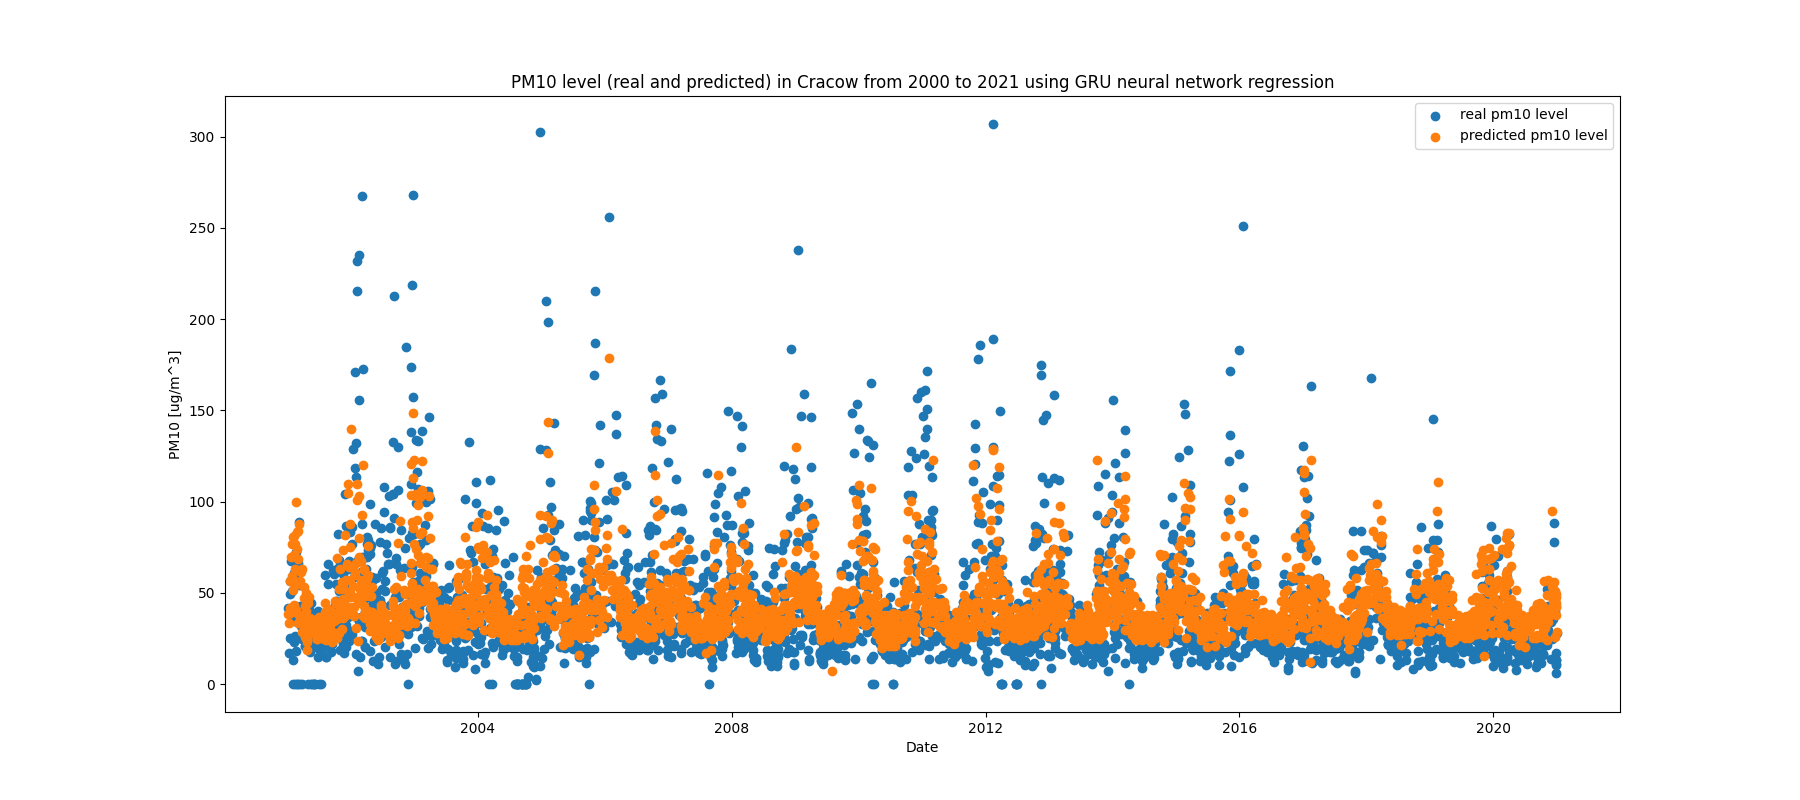
\includegraphics[scale=0.4]{GRU_512.png}}
	\caption{Zestawienie wyników sieci GRU z 512 neuronami w warstwie ukrytej z prawdziwymi obserwacjami}
	\label{figure:gru_512}
\end{figure}
\FloatBarrier

Na \autoref{figure:gru_2}, \autoref{figure:gru_64} oraz \autoref{figure:gru_512} przedstawione zostały zestawienia wyników predykcji z realnymi danymi obserwacyjnymi. Na wykresach tych oś x reprezentuje czas w dniach, oś y natomiast reprezentuje poziom zanieczyszczenia pyłem PM10. Predykcje są zaznaczane kolorem pomarańczowym, a wartości obserwowane kolorem niebieskim. Dokładna analiza tych wykresów wraz ze zrozumieniem wcześniej omówionej \autoref{table:gru} z parametrami opisującym jakość wyników powinna umożliwić wybór optymalnej konfiguracji sieci neuronowej opartej o Gated Recurrent Unit.

Na \autoref{figure:gru_2} doskonale widać jak zachowuje się sieć nie posiadająca wystarczającej możliwości przetwarzania informacji w procesie predykcyjnym. Utworzone przez z nią predykcje zupełnie nie pokrywają się z danymi wejściowymi. Taki model jest przeciążony złożonością rozwiązywanego problemu i nie nadaje się w żadnym wypadku do zastosowania w tym konkretnym problemie. Zajmowanie się tak prostym modelem w analizie, biorąc jego całkowitą niemożność rozwiązania postawionego mu problemu wydaje się nieprzydatne. Być może tak mała warstwa ukryta będzie adekwatna w innych przypadkach, ale w tej pracy nie może zostać wykorzystana. Z obserwacji jej można jednak wyciągnąć ważne wnioski i należyte omówienie ich prowadzi do lepszego zrozumienia problemu. 

Zdecydowanie bardziej ciekawe w kontekście dalszej analizy są sieci neuronowe, których predykcje są obrazowane na \autoref{figure:gru_64} oraz \autoref{figure:gru_512}. Obie sieci ze znacznie większą dokładnością od poprzedniego odwzorowują zbiór wejściowy i zapewniają względnie akceptowalną jakość predykcji. Porównanie ich ze sobą może posłużyć jako podstawa do wyciągnięcia interesujących badawczo wniosków na temat sieci neuronowych w architekturze GRU. 

Wyraźnie widoczne jest podobieństwo obu wykresów, obserwacja ta znajduje również odzwierciedlenie w wynikach przedstawionych w \autoref{table:gru}. Odpowiada ono również charakterowi relacji pomiędzy dokładnością wyników a liczbą neuronów warstwy ukrytej prezentowanej na \autoref{figure:gru_neurons}. Widoczna jest poprawa predykcji modelu z 1024 neuronami w warstwie ukrytej - poprawnie przewiduje on większą liczbę bardzo wysokich poziomów zanieczyszczeń, podchodzi do średnich wartości zanieczyszczeń z większym poziomem zniuansowania.

To podobieństwo może być również traktowane jako potencjalny problem biorąc pod uwagę wzrost złożoności obliczeniowej wraz ze wzrostem liczby neuronów. Jeżeli czterokrotny wzrost liczby neuronów nie daje proporcjonalnie lepszych wyników to warto zastanowić się czy takie dodatkowe skomplikowanie modelu ma jakąkolwiek wartość. Wydaje się być rozsądnym przedsięwzięciem próba odnalezienia optymalnej wielkości warstwy ukrytej dla rozwiązywanego problemu. 

Obserwując wszystkie trzy rysunki można stwierdzić fakt nie radzenia sobie sieci z odczytywaniem trendu w danych wejściowych. Znając architekturę sieci oraz założenia, na których została ona zbudowana, może być to zaskakujące. Trzeba jednak uczciwie stwierdzić, że trend ten jest stosunkowo niewielkich rozmiarów co może znacząco utrudniać wykrycie go przez sieć. 

\subsubsection{Zestawienie otrzymanych wyników}
Kluczowym punktem tej pracy jest zestawienie ze sobą wyników różnych metod predykcyjnych i przeanalizowanie jakości zwracanych przez nie rozwiązań. Czynności te pozwolą zbudować podstawy do wyciągania wniosków odnośnie przydatności poszczególnych metod do predykcji szeregów czasowych. W tej podsekcji porównane zostaną wyniki, które były dokładnie przedyskutowane w poprzednich podsekcjach oraz zbudowane zostaną podstawy merytoryczne do dalszej pracy i wyciągania wniosków. 

W trakcie poprzednich analiz poszczególnych modeli w izolacji można było stracić z oczu cel tej pracy i zapomnieć jakie metody predykcyjne są analizowane w ramach tej pracy. Być może z tego powodu warte jest przypomnienie metod, porównywanych w dalszej części tego podrozdziału, są to:
\begin{itemize}
	\item Regresja liniowa
	\item Regresja z wykorzystaniem drzew decyzyjnych
	\item Predykcja z wykorzystaniem prostej sieci neuronowej
	\item Predykcja z wykorzystaniem sieci neuronowej opartej na architekturze Long Short-Term Memory (LSTM)
	\item Predykcja z wykorzystaniem sieci neuronowej opartej na architekturze Gated Recurrent Memory (GRU)
\end{itemize}

W celu umożliwienia dyskusji nad jakością wyników uzyskiwanych przez różne metody stworzone zostało tabelaryczne zestawienia w postaci \autoref{table:models_comparison}. Aby uniknąć niesprawiedliwych porównań w zestawieniu ujęte zostały najbardziej optymalne konfiguracje każdej metody. Porównywanie najgorszych możliwych kombinacji parametrów jednej metody z najlepszymi parametrami innej mogłoby prowadzić do nieszczerej oceny faktycznej jakości predykcji zwracanych przez model. Dla drzew decyzyjnych wybrane zostało drzewo o głębokości 5, gdyż z \autoref{figure:treer2} wynika, że jest to optymalna głębokość drzewa. 

W przypadku sieci neuronowych proces dobierania optymalnych parametrów był nieco bardziej skomplikowany. O ile największa możliwa liczba neuronów w warstwie ukrytej zwracała najlepsze wyniki to zawsze zużywała najwięcej zasobów obliczeniowych. Mając na uwadze zwiększone zużycie zasobów oraz brak drastycznej poprawy wyników poprzez zwiększenie wielkości sieci podjęta została decyzja o wykorzystaniu sieci neuronowych z 256 neuronami w warstwie ukrytej. Jest to liczba neuronów, gdzie przy wzroście neuronów nie jest już odnotowywana gwałtowna poprawa zwracanych wyników oraz czas treningu sieci jest względnie akceptowalny.


\begin{table}[h!]
	\centering
	\begin{tabular}{|c|c|c|c|c|}
		\hline
		Metoda predykcji & $R^2$ & MSE & RMSE & Willmott \\
		\hline
		Regresja liniowa & 0.3230 & 1386.2897 & 37.2329 & 0.6719 \\
		Drzewa decyzyjne & 0.3276 & 1376.8134 & 37.1054 & 0.6878\\
		Prosta sieć rekurencyjna & 0.3865  & 1256.3483 & 35.4450 & 0.7190 \\
		Sieć LSTM & 0.3948  & 1239.2538 & 35.2030 & 0.7154 \\
		Sieć GRU & 0.3987  & 1231.2979 & 35.0899 & 0.7053 \\
		\hline
	\end{tabular}
	\caption{Zestawienie parametrów opisujących jakość predykcji różnych metod}
	\label{table:models_comparison}
\end{table}

Widoczny jest subtelny przeskok w jakościach predykcji pomiędzy metodami klasycznymi (regresja liniowa, drzewa decyzyjne) oraz tymi opartymi na rekurencyjnych sieciach neuronowych. Nie jest to być może duży przeskok, ale jest na tyle znaczący, że nie można go pominąć w dalszych rozważaniach. Kwestia tego czy ta poprawa parametrów jest wystarczająca, aby usprawiedliwić używanie bardziej skomplikowanych sieci neuronowych jest dyskusyjna i zostanie dokładniej omówiona w \hyperlink{section.6}{rozdziale 6}. Kwestia ta może również dodatkowo komplikować większa ilość badań i szeroko rozumiane lepsze zrozumienie działania metod klasycznych. W celu zbudowania adekwatnej podstawy do dalszego wnioskowania należy przeanalizować inne sposoby porównywania jakości predykcji. 

Nie widać podobnych przeskoków w wartościach parametrów trzech różnych rekurencyjnych sieci neuronowych. W zależności od tego, na którym parametrze skupiona zostanie uwaga, wyciągnięte mogą być różne wnioski odnośnie relatywnej jakości predykcji z różnych metod. Z tego powodu w celu zbudowania podstaw do adekwatnego porównania wykorzystywanych sieci neuronowych należy spojrzeć na więcej aspektów działania modeli.

\begin{figure}[!ht]
	\centering
	\makebox[0pt]{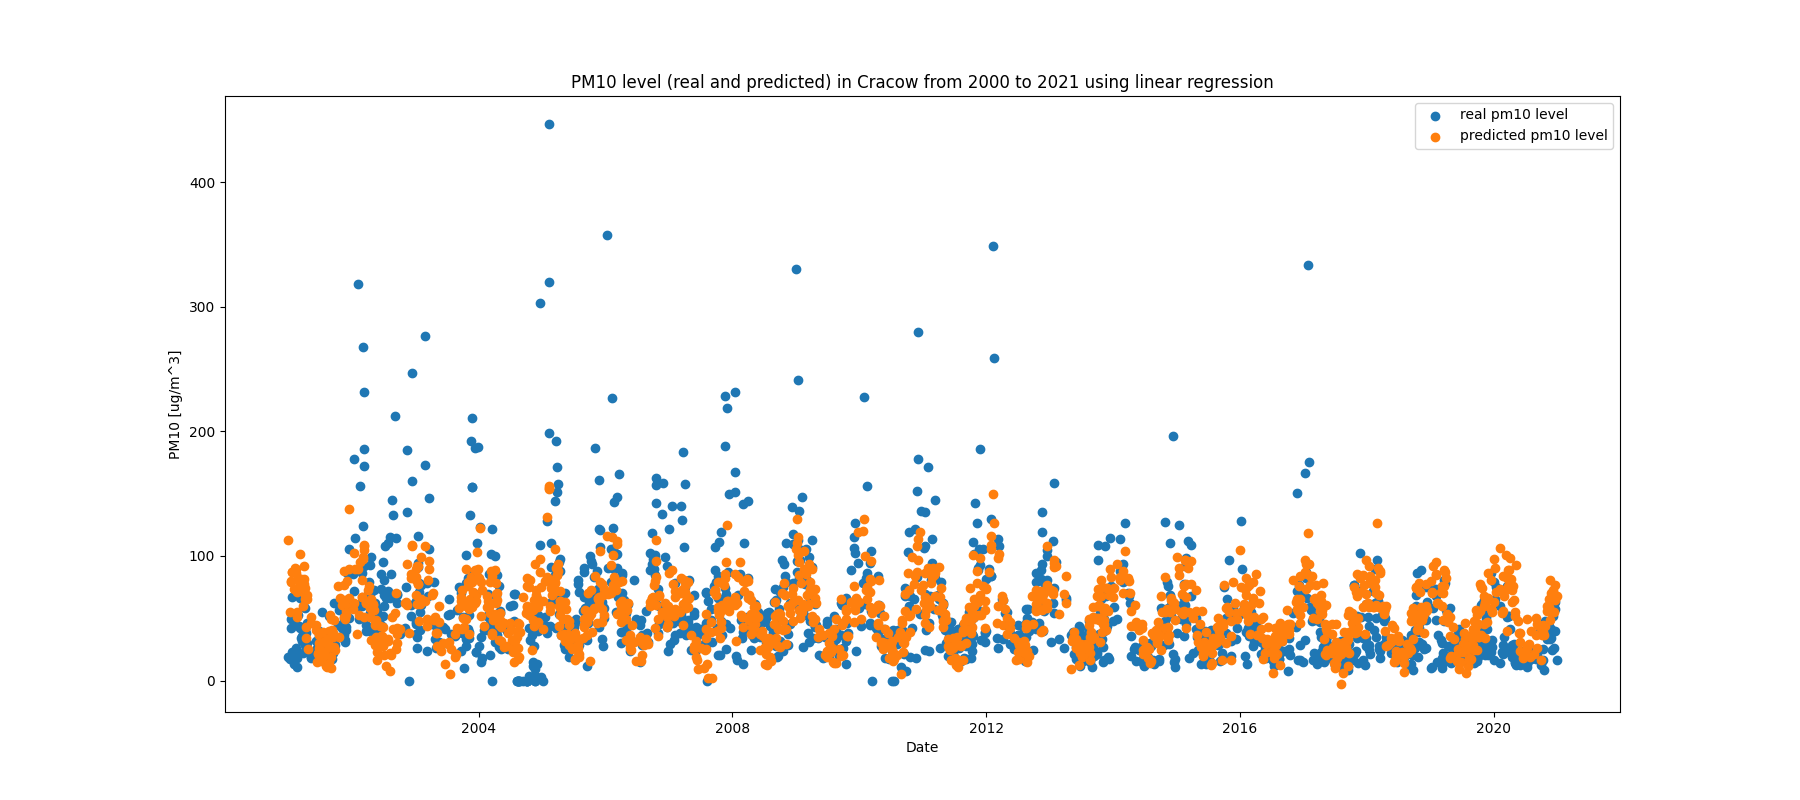
\includegraphics[scale=0.4]{linear.png}}
	\caption{Zestawienie wyników regresji liniowej z prawdziwymi obserwacjami}
	\label{figure:linear_comparison}
\end{figure}
\FloatBarrier
\begin{figure}[!ht]
	\centering
	\makebox[0pt]{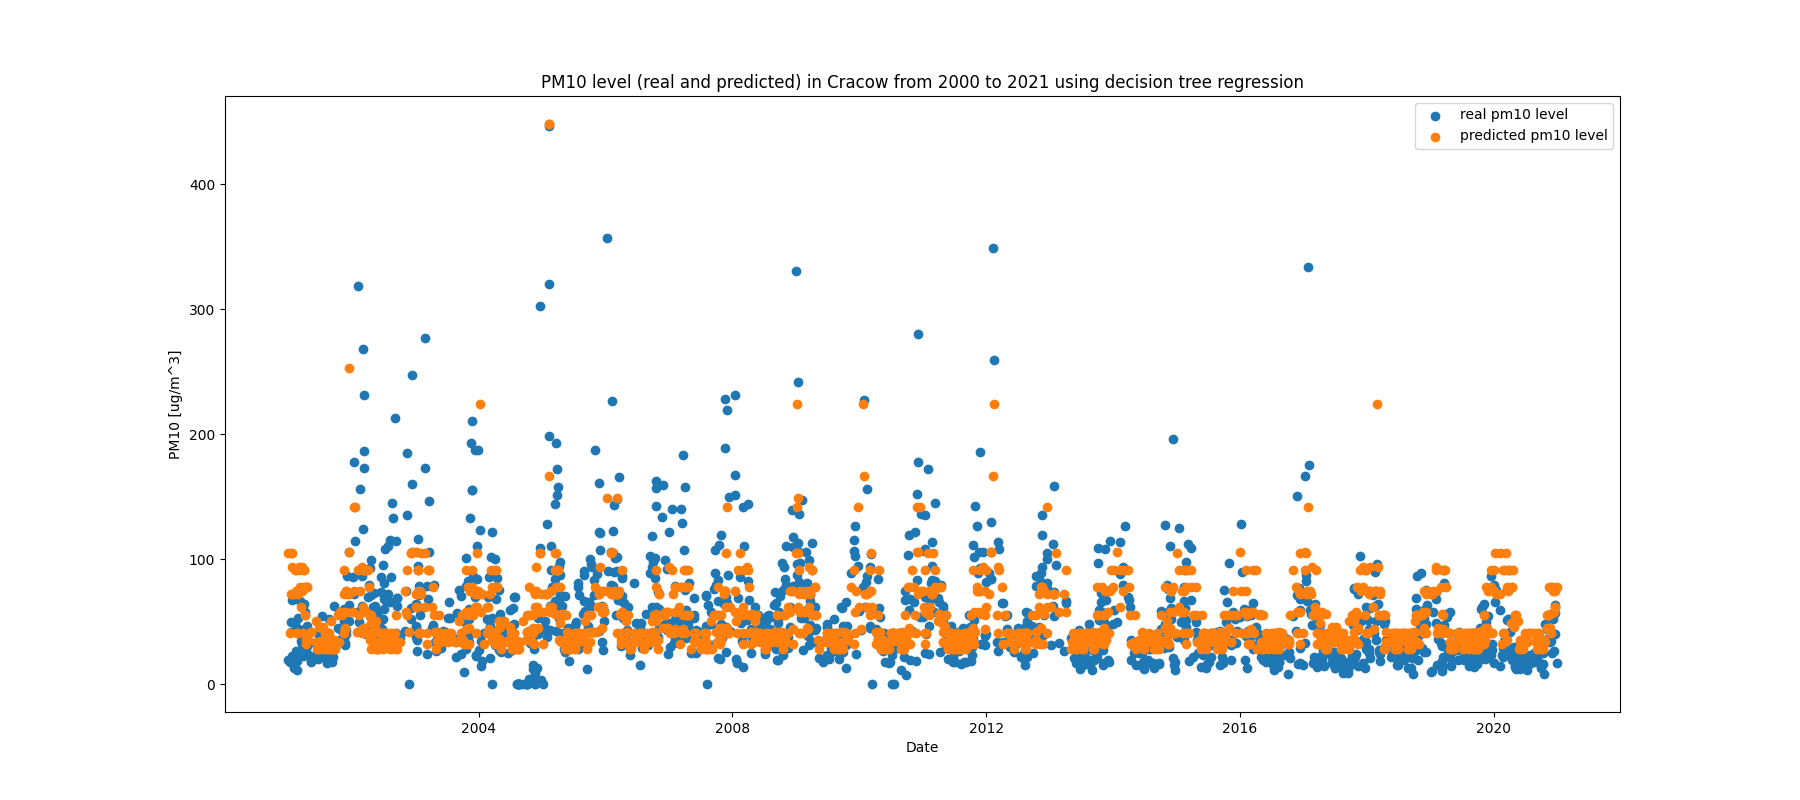
\includegraphics[scale=0.4]{decission_tree_5.png}}
	\caption{Zestawienie wyników drzewa o głębokości 5 z prawdziwymi obserwacjami}
	\label{figure:tree_comparison}
\end{figure}
\FloatBarrier
\begin{figure}[!ht]
	\centering
	\makebox[0pt]{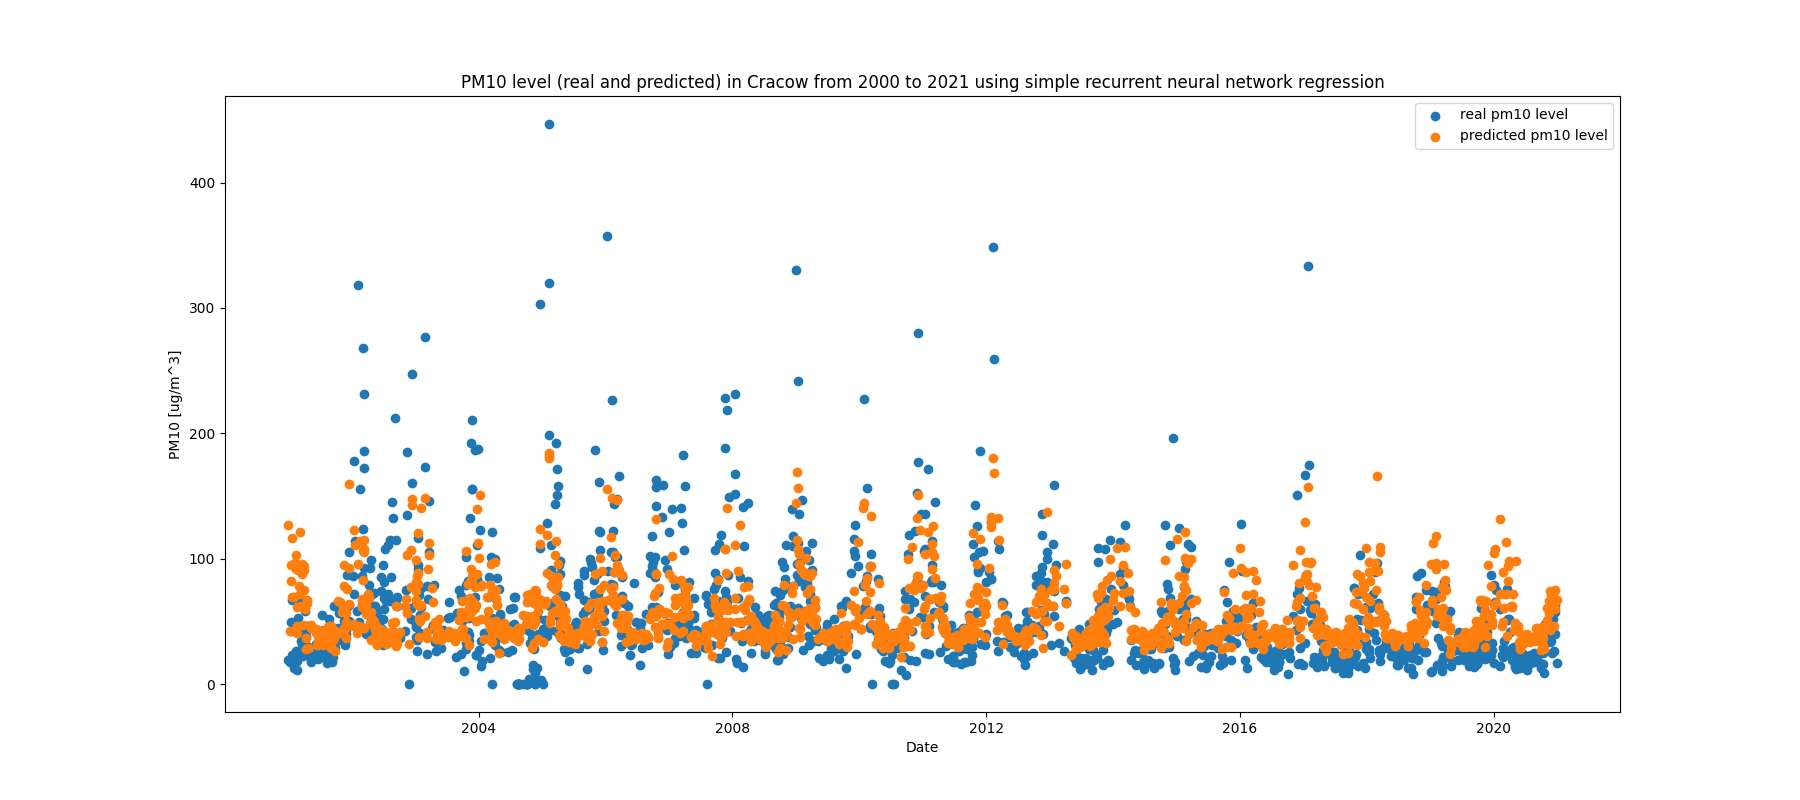
\includegraphics[scale=0.4]{SimpleRNN_256.png}}
	\caption{Zestawienie wyników prostej sieci neuronowej z 256 neuronami w warstwie ukrytej z prawdziwymi obserwacjami}
	\label{figure:simple_rnn_comparison}
\end{figure}
\FloatBarrier
\begin{figure}[!ht]
	\centering
	\makebox[0pt]{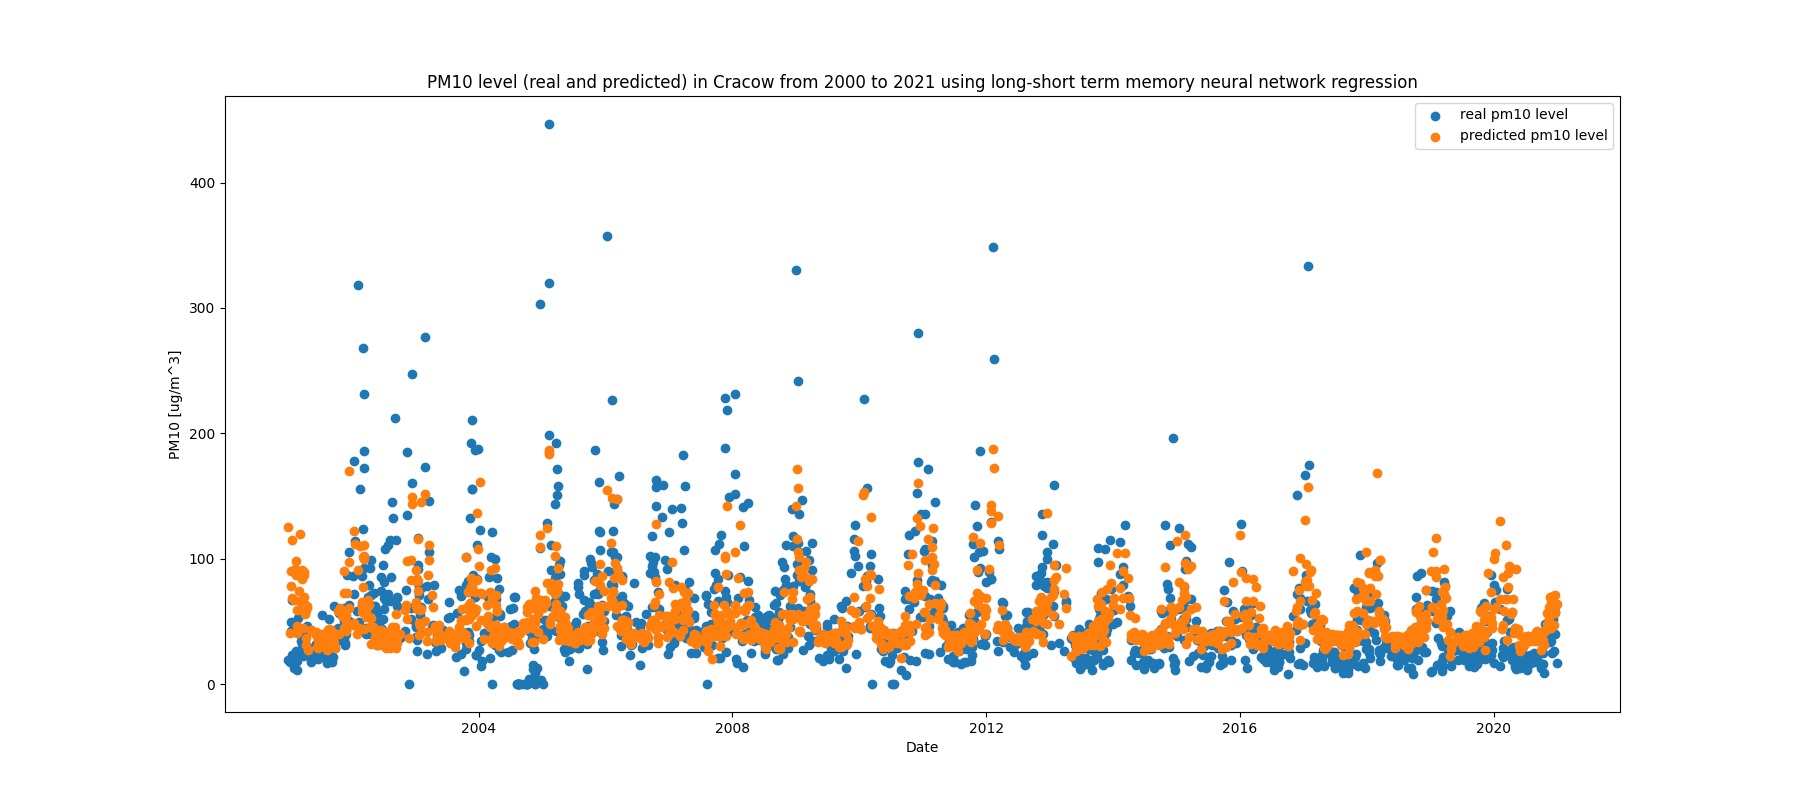
\includegraphics[scale=0.4]{LSTM_256.png}}
	\caption{Zestawienie wyników sieci neuronowej opartej na architekturze LSTM z 256 neuronami w warstwie ukrytej z prawdziwymi obserwacjami}
	\label{figure:lstm_comparison}
\end{figure}
\FloatBarrier
\begin{figure}[!ht]
	\centering
	\makebox[0pt]{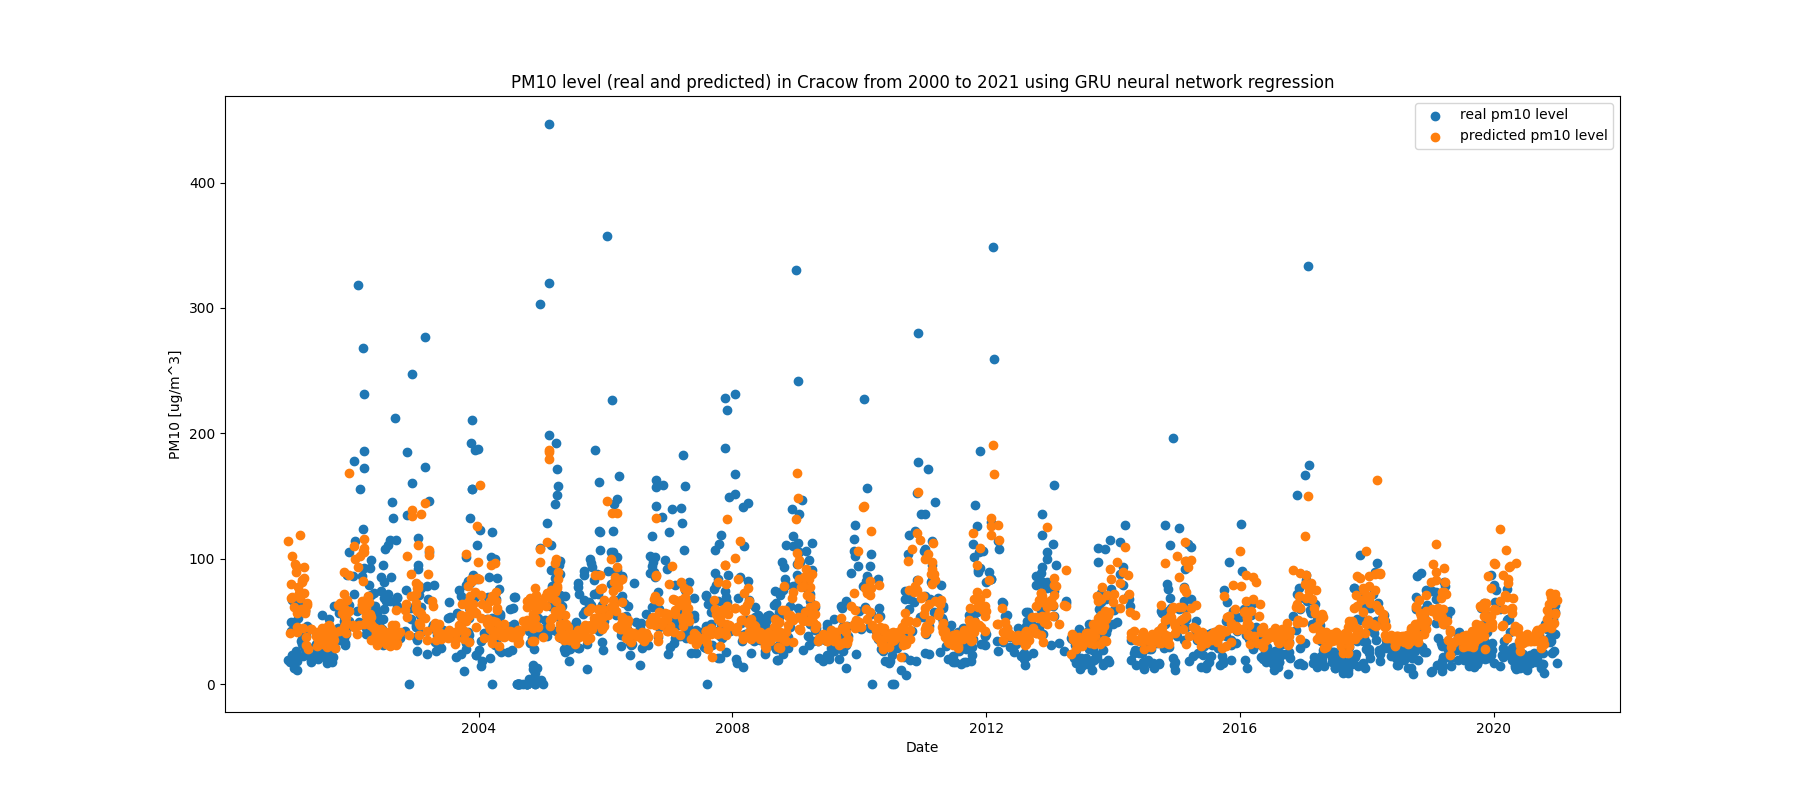
\includegraphics[scale=0.4]{GRU_256.png}}
	\caption{Zestawienie wyników sieci neuronowej opartej na architekturze GRU z 256 neuronami w warstwie ukrytej z prawdziwymi obserwacjami}
	\label{figure:gru_comparison}
\end{figure}
\FloatBarrier

Analiza graficznych zestawień wyników modeli predykcyjnych z pierwotnymi danymi może okazać się przydatnym narzędziem do tworzenia podstaw do wyciągania wniosków w dalszej części pracy. Na \autoref{figure:linear_comparison}, \autoref{figure:tree_comparison}, \autoref{figure:simple_rnn_comparison}, \autoref{figure:lstm_comparison} oraz \autoref{figure:gru_comparison} są prezentowane te właśnie zestawienia. Zostaną one teraz omówione i przeanalizowane w poszukiwaniu czynników rozróżniających modele.

Najbardziej od innych rysunków odstępuje \autoref{figure:tree_comparison} i wydaje się sensowym zająć się nim w pierwszej kolejności. Widać wyraźnie, że w porównaniu do innych metod predykcje tego modelu są bardziej ,,nieciągłe''. Ze względu na problem zbytniego dopasowywania do danych wejściowych głębokość drzewa została ograniczona do tylko 5 poziomów. Oznacza to, że model posiada jedynie $2^5$ poziomów zanieczyszczeń, które może określić na podstawie danych klimatycznych. Ograniczenie to wydaje się stawiać model na pozycji gorszej od alternatyw biorąc pod uwagę charakterystykę szeregu czasowego, którego próby przewidywania są podejmowane. 

Wyniki drugiej wykorzystywanej klasycznej metody predykcyjnej czyli regresji liniowej przedstawionej na \autoref{figure:linear_comparison} również wydają się różnić od wyników metod opartych na sieciach neuronowych. Regresja liniowa trzyma się bardzo mocno najczęściej występujących wartości parametrów i co do zasady osiąga w tym dobre wyniki. Problematyczny w kontekście wykorzystania tej metody może być fakt, że w porównaniu do reszty bardzo mało uwagi poświęca ona bardzo wysokim poziomom zanieczyszczeń. Pozostałe metody próbują dopasować swoje predykcje do występowania tych nietypowych stężeń pyłu PM10 co może być potencjalnie odczytywane jako ich zaleta nad regresją liniową. 

Takie porównania wykresów obrazujących wyniki klasycznych metod predykcyjnych do sieci neuronowych wydają się utwierdzać poprawność obserwacji wynikających z analizy \autoref{table:models_comparison} o nieco niższej jakości otrzymywanych przez nie wyników. Obserwacja ta ma potencjał do umożliwiania wyciągnięcia interesujących wniosków odnośnie sensowności wykorzystywania rekurencyjnych sieci neuronowych do predykcji szeregów czasowych. Wnioski te zostaną przedstawione w \hyperlink{section.6}{rozdziale 6}.

Podobnie jak przy porównaniu parametrów opisujących jakość wyników, tak samo w analizie wykresów wyników sieci neuronowych nie widać radykalnych różnic pomiędzy różnymi architekturami sieci. Nie należy jednak pomijać tych różnic. Nawet jeżeli nie są one najbardziej widoczne to mogą mieć znaczenie podczas prób wyciągania wniosków odnośnie wydajności poszczególnych modeli. 

Wszystkie modele sieci próbują dopasować się do bardzo wysokich poziomów zanieczyszczeń, ale różnią się stopniem tego dopasowania. Prosta sieć rekurencyjna dopasowuje się słabiej niż sieć typu Long Short-Term Memory, natomiast sieć typu Gated Recurrent Unit dopasowuje się najlepiej z pośród wszystkich trzech sieci. Nie są to duże różnice i pamiętając obserwację z analizy wpływu liczby neuronów w warstwie ukrytej na jakość uzyskiwanych wyników, nasuwa się pytanie czy ta obserwacja może wyjaśniać istnienie tych różnic.

\begin{figure}[!ht]
	\centering
	\makebox[0pt]{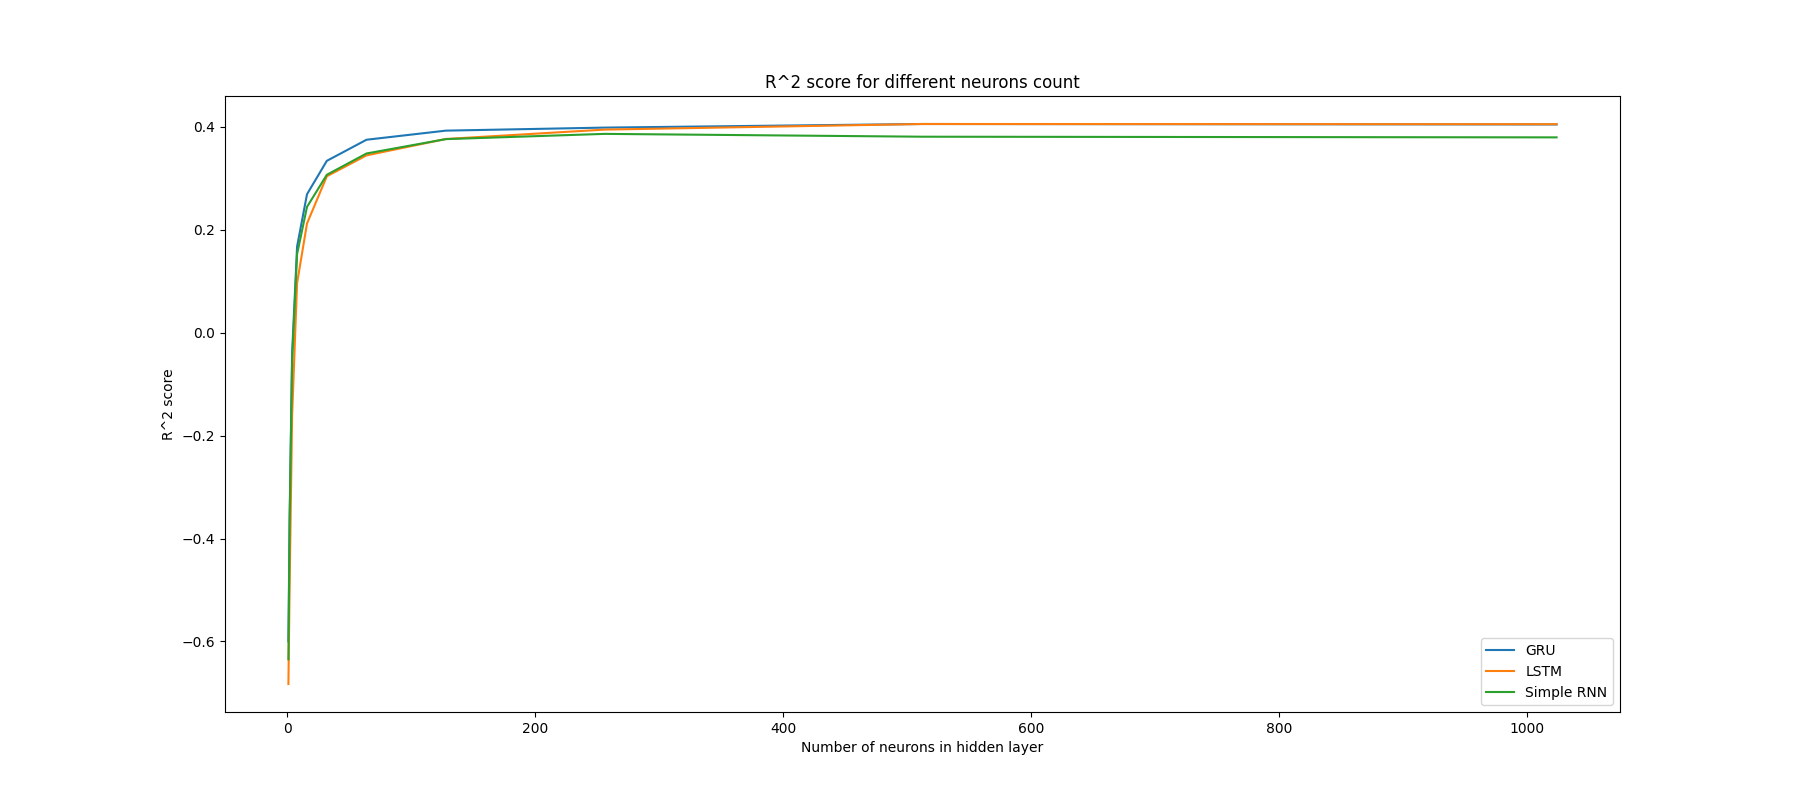
\includegraphics[scale=0.35]{neurons_comparison.png}}
	\caption{Wynik testu $R^2$ w zależności do liczby neuronów w warstwie ukrytej}
	\label{figure:neurons_comparison}
\end{figure}
\FloatBarrier

W celu rozwiania tej wątpliwości sporządzony został \autoref{figure:neurons_comparison} obrazujący zmianę wyniku testu $R^2$ dla różnej liczby neuronów w warstwie ukrytej dla wszystkich analizowanych sieci rekurencyjnych. Kolorem zielonym prezentowana jest ta zmiana dla prostej sieci rekurencyjnej, kolorem pomarańczowym dla sieci opartej na architekturze Long Short-Term Memory, a kolorem niebieskim dla sieci opartej na architekturze Gated Recurrent Unit. Wykres ten umożliwia wyróżnienie kilku ważnych obserwacji:
\begin{itemize}
	\item Prosta sieć rekurencyjna najwolniej reaguje na wzrost liczby neuronów i osiąga ostatecznie najgorszy wynik.
	\item Sieć typu LSTM zaczyna z najgorszym wynikiem i reaguje na wzrost liczby neuronów z podobną prędkością co prosta sieć neuronowa, ale osiąga ostatecznie lepszy wynik.
	\item Sieć typu GRU zaczyna z najlepszym wynikiem i reaguje najszybciej na wzrost liczby neuronów. Ostatecznie osiąga najlepszy wynik na równi z siecią typu LSTM, ale robi to szybciej od drugiej sieci. 
\end{itemize}
Obserwacje te wraz ze świadomością wzrostu narzutu obliczeniowego przy wzroście liczby neuronów może być dobrą podstawą do wyciągania wniosków odnośnie relatywnej przydatności rekurencyjnych sieci neuronowych do predykcji szeregów czasowych.

Innym aspektem wydajności sieci neuronowej przydatnym w formułowaniu wniosków jest prędkość uczenia sieci, rozumiana jako ilość epok uczących potrzebnych do osiągnięcia optymalnego poziomu wyuczenia. Przez optymalny poziom wyuczenia rozumiemy moment, w którym dodanie kolejnej epoki uczącej nie wpływa w znaczący sposób na osiągane wyniki. Zjawisko to można ewaluować poprzez analizę funkcji błędu w zależności od epoki uczącej. 

\begin{figure}[!ht]
	\centering
	\makebox[0pt]{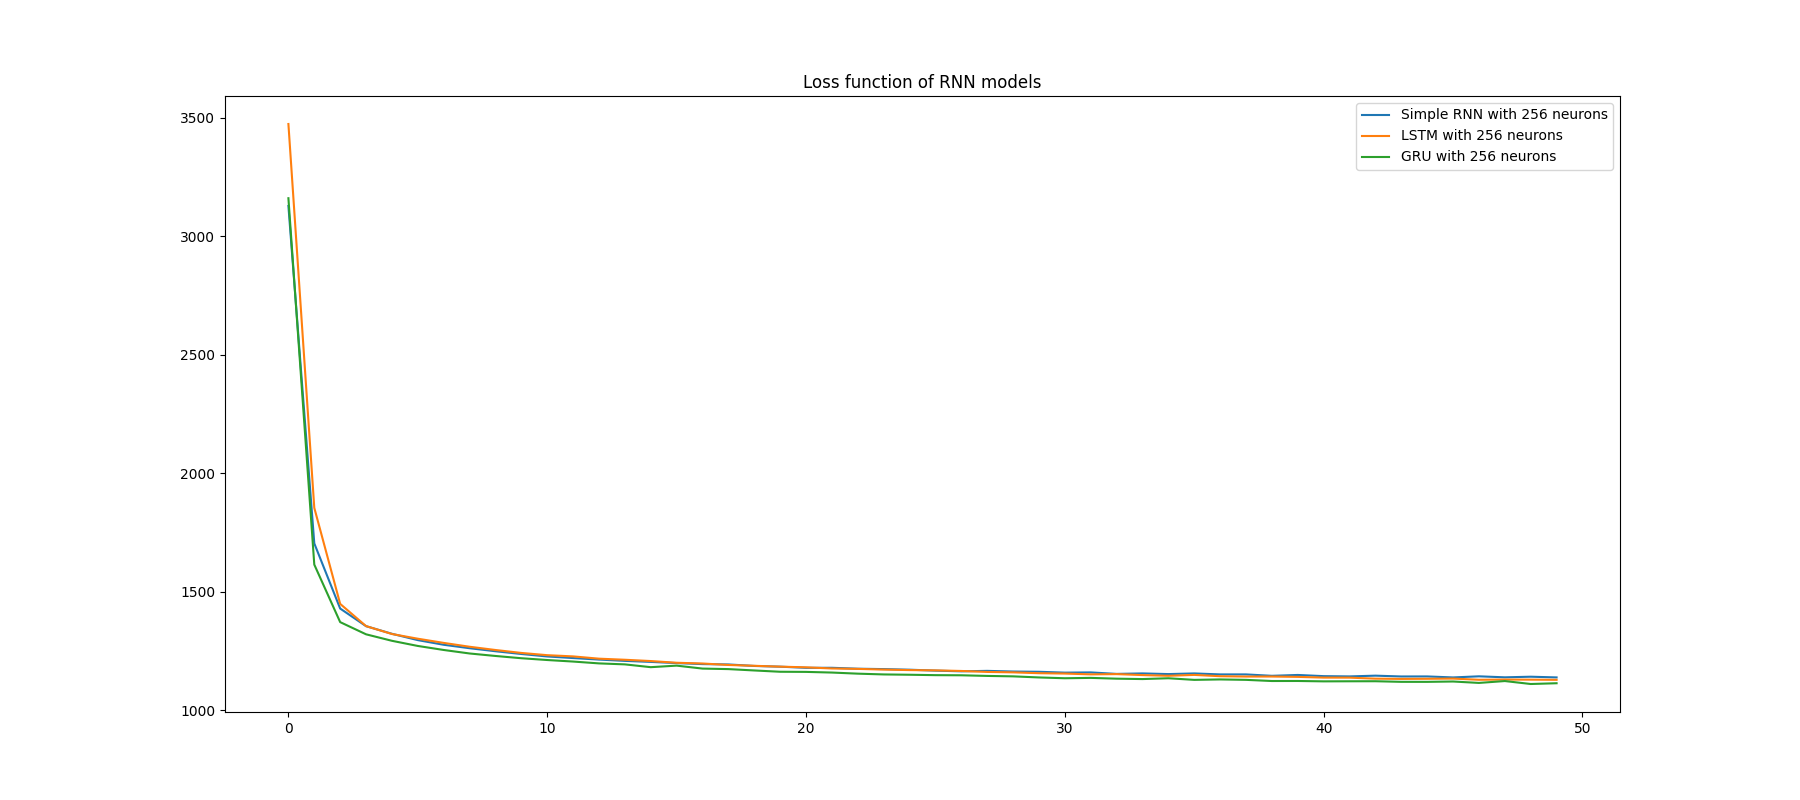
\includegraphics[scale=0.4]{loss_history.png}}
	\caption{Wynik testu $R^2$ w zależności do liczby neuronów w warstwie ukrytej}
	\label{figure:loss_history}
\end{figure}
\FloatBarrier

Na \autoref{figure:loss_history} przedstawiona została taka zależność dla wszystkich porównywanych ze sobą sieci neuronowych. Kolorem niebieskim reprezentowana jest prosta sieć neuronowa, kolorem pomarańczowym sieć oparta na architekturze Long Short-Term Memory, a kolorem zielonym sieć oparta na architekturze Gated Recurrent Unit. Na osi x reprezentowane są kolejne epoki uczenia sieci, a na osi y wartość funkcji błędu. Jako funkcja błędu w procesie uczenia wykorzystywana była wartość błędu średniokwadratowego w danej epoce. 

Wykres ten umożliwia odnotowanie kilku potencjalnie przydatnych przy wyciąganiu wniosków informacji:
\begin{itemize}
	\item Prosta sieć neuronowa rozpoczyna naukę z najmniejszą wartością błędu średniokwadratowego i uczy się średnio szybko w porównaniu do innych sieci. Ostatecznie osiąga najgorszy wynik ze wszystkich sieci, ale różnice wyników końcowych są bardzo niewielkie.
	\item Sieć oparta o architekturę LSTM rozpoczyna naukę z największą wartością błędu średniokwadratowego i uczy się stosunkowo wolno. Ostatecznie udaje jej się jednak otrzymać lepszy wynik od prostej sieci neuronowej, chociaż jak zostało zauważone zostało wcześniej ostatecznie różnice są bardzo małe.
	\item Sieć oparta na architekturze GRU rozpoczyna naukę z nieco większą wartością błędu od sieci prostej, ale uczy się zdecydowanie najszybciej. Dzięki temu osiąga najlepszy wynik, ale różnica tego ostatecznego wyniku od reszty sieci jest niewielka. 
\end{itemize}

Obserwacje te w dużej mierze pokrywają się z tymi poczynionymi przy analizie wpływu liczby neuronów na jakość wyników. Pozwala to wierzyć w pewną przewagę wydajnościową sieci Gated Recurrent Unit nad pozostałymi. Przewaga ta została wykorzystana w dalszych badaniach. Mając na uwadze czas potrzebny do zbadania skalowalności modelu przyjęte zostało założenie, że wybór wydajniejszej sieci skróci czas potrzebny do prawidłowego przeprowadzenia takiego badania. Wyniki uzyskane w takiej analizie skalowalności zostaną przedstawione w \hyperlink{subsection.5.2}{podrozdziale 5.2}.

\subsection{Badanie skalowalności modelu GRU}

W ramach badania skalowalności sieci neuronowej opartej na architekturze Gated Recurrent Unit zebrane zostały takie same dane jak przy poprzednich badaniach. W ramach tego podrozdziału zostaną one przedstawione i przeanalizowane w celu stworzenia podstaw do wyciągania wniosków odnośnie przydatności tej sieci do predykcji szeregów czasowych. 

W \autoref{table:scale_comparison} zestawione zostały wartości parametrów opisujących jakość wyników predykcji sieci neuronowej w architekturze GRU. Są one ukazane w zależności od liczby analizowanych punktów pomiarowych i co za tym idzie wielkości szeregu, dla którego prowadzona jest predykcja. Bliższa inspekcja tych parametrów może pozwolić na zrozumienie wpływu wielkości zbioru danych wejściowych na wydajność sieci. W trakcie tworzenia tabeli pominięte zostały wyniki punktów pomiarowych mających bardzo niewiele danych mogących zostać wykorzystanych w szeregu. Wynika to z założenia, że zmiana wyników była na tyle niewielka, że uwzględnienie ich nie byłoby wartościowe dla zestawienia. 

Podczas obserwacji wyników można zauważyć bardzo wyraźny i co do zasady niezachwiany trend spadkowy błędu średniokwadratowego. Relacja ta została przedstawiona na \autoref{figure:scale_mse} i wyraźnie maleje ze wzrostem długości badanego szeregu. Wydaje się to utwierdzać przekonanie o dobrej skalowalności stworzonego modelu. Utwierdzenie to jest tym mocniejsze, że to właśnie błąd średniokwadratowy jest używany jako funkcja błędu podczas uczenia modelu. Oznacza to, że zwiększenie liczy danych wejściowych ma pozytywny wpływ na jakość procesu uczenia. 

Jednak obserwacje wyniku testu $R^2$ oraz wartości indeksu Willmott'a zdają się nie dawać tak optymistycznych rezultatów. Co do zasady fluktuują one wokół jednej wartości, 0.35 dla $R^2$ i 0.70 dla indeksu Willmott'a. Fluktuacje te dla tego drugiego parametru przedstawione są na \autoref{figure:scale_willmott}. Dla pewnych długości szeregu czasowego, wartości te są lepsze lub gorsze, ale nie widać długotrwałego trendu opisującego poprawnie tendencję tych wyników. Nie widać zatem pozytywnego wpływu długości szeregu na wartości tych parametrów, ale nie widać też znaczącego pogorszenia pomimo dziesięciokrotnego wzrostu wielkości zbioru wejściowego. 

Zestawienie to może jest interesujące, ale nasuwają się pytania czy uzyskane relacje utrzymałyby się przy jeszcze większym wzroście długości szeregu. Niemożność powiększenia go korzystając z posiadanych danych obserwacyjnych nie pozwala jednoznacznie tego zweryfikować. 

\begin{table}[h!]
	\centering
	\begin{tabular}{|c|c|c|c|c|c|}
		\hline
		P. pomiarowe & Wielkość szeregu & $R^2$ & MSE & RMSE & Willmott \\
		\hline
		1  & 7193  & 0.4166 & 1183.4677 & 34.4016 & 0.7386 \\
		2  & 14372 & 0.3279 & 995.0935  & 31.5451 & 0.6273 \\
		3  & 14929 & 0.3308 & 915.0519  & 30.2498 & 0.6676 \\
		4  & 18768 & 0.3914 & 924.4917  & 30.4055 & 0.7197 \\
		5  & 18880 & 0.3773 & 887.3174  & 29.7879 & 0.7034 \\
		6  & 20877 & 0.3838 & 845.1975  & 29.0723 & 0.7224 \\
		7  & 23536 & 0.4125 & 827.2894  & 28.7626 & 0.7334 \\
		8  & 28388 & 0.3493 & 756.8922  & 27.5117 & 0.7163 \\
		9  & 31291 & 0.3612 & 725.9746  & 26.9439 & 0.7304 \\
		10 & 33225 & 0.3326 & 771.0799  & 27.7683 & 0.7008 \\
		11 & 37202 & 0.3401 & 760.2995  & 27.5735 & 0.7156 \\
		12 & 38150 & 0.3396 & 758.2695  & 27.5367 & 0.7062 \\
		13 & 41828 & 0.3774 & 755.3431  & 27.4835 & 0.7099 \\
		14 & 45375 & 0.3797 & 716.1558  & 26.7611 & 0.7087 \\
		15 & 51034 & 0.3569 & 710.9420  & 26.6635 & 0.7036 \\
		16 & 56810 & 0.3562 & 672.1225  & 25.9253 & 0.7067 \\
		17 & 60145 & 0.3594 & 645.1233  & 25.3993 & 0.7071 \\
		18 & 66146 & 0.3480 & 619.7134  & 24.8940 & 0.6912 \\
		19 & 68729 & 0.3403 & 632.2250  & 25.1441 & 0.6994 \\
		20 & 71207 & 0.3605 & 643.4277  & 25.3659 & 0.7110 \\
		21 & 74181 & 0.3451 & 626.0303  & 25.0206 & 0.7018 \\
		\hline
	\end{tabular}
	\caption{Zestawienie parametrów opisujących jakość predykcji  zależności od wielości szeregu}
	\label{table:scale_comparison}
\end{table}


\begin{figure}[!ht]
\centering
\makebox[0pt]{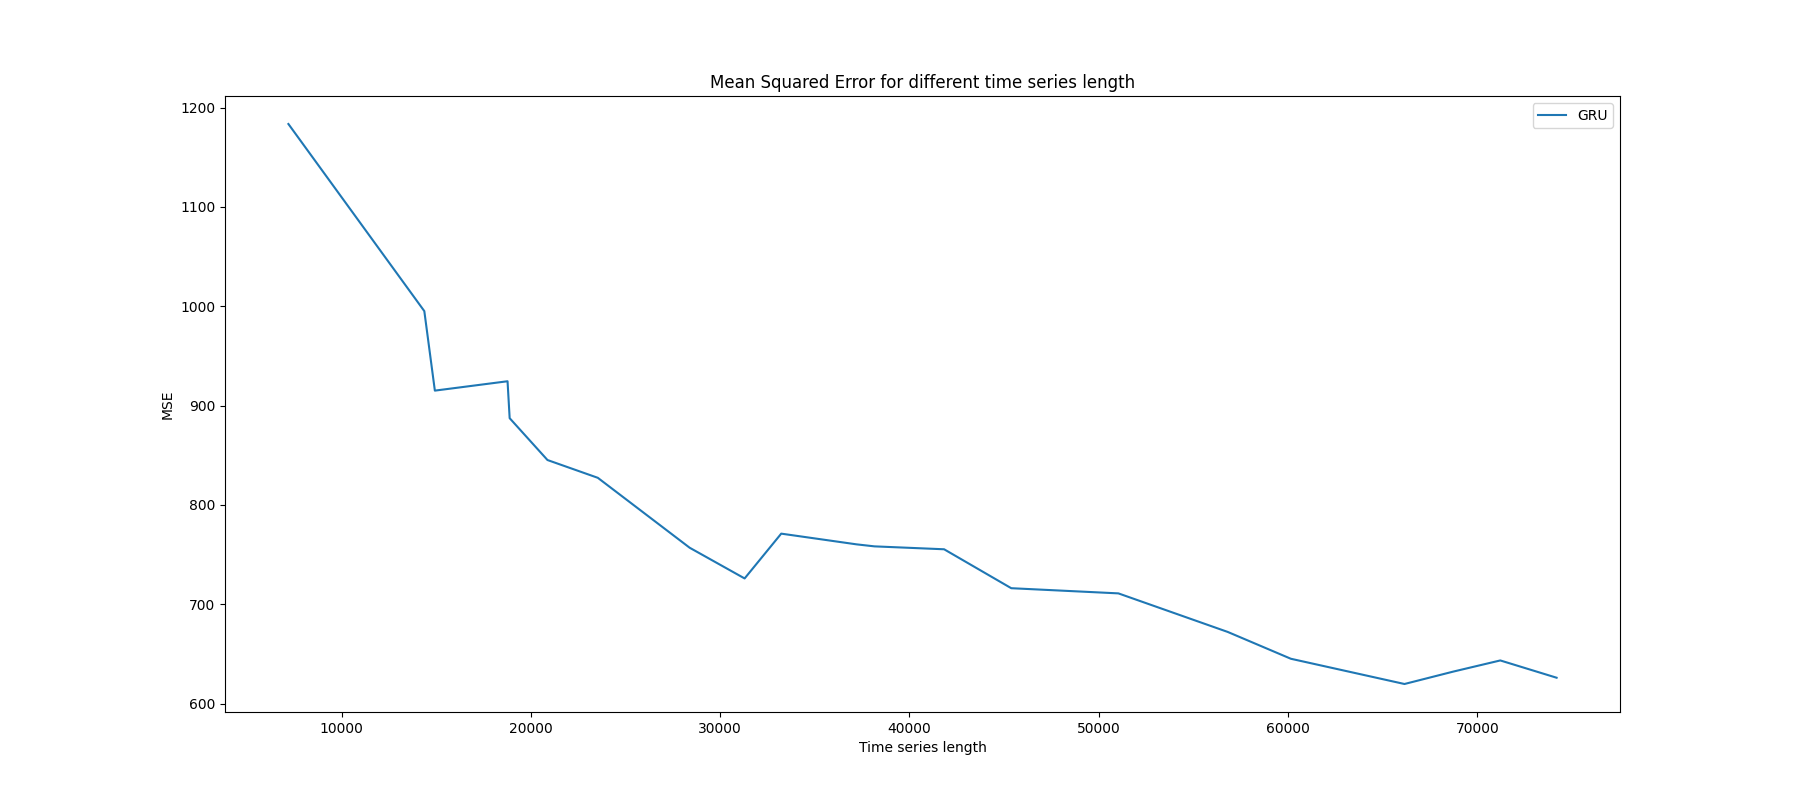
\includegraphics[scale=0.3]{scale_mse.png}}
\caption{Błąd średniokwadratowy w zależności od długości szeregu}
\label{figure:scale_mse}
\end{figure}
\FloatBarrier

\begin{figure}[!ht]
	\centering
	\makebox[0pt]{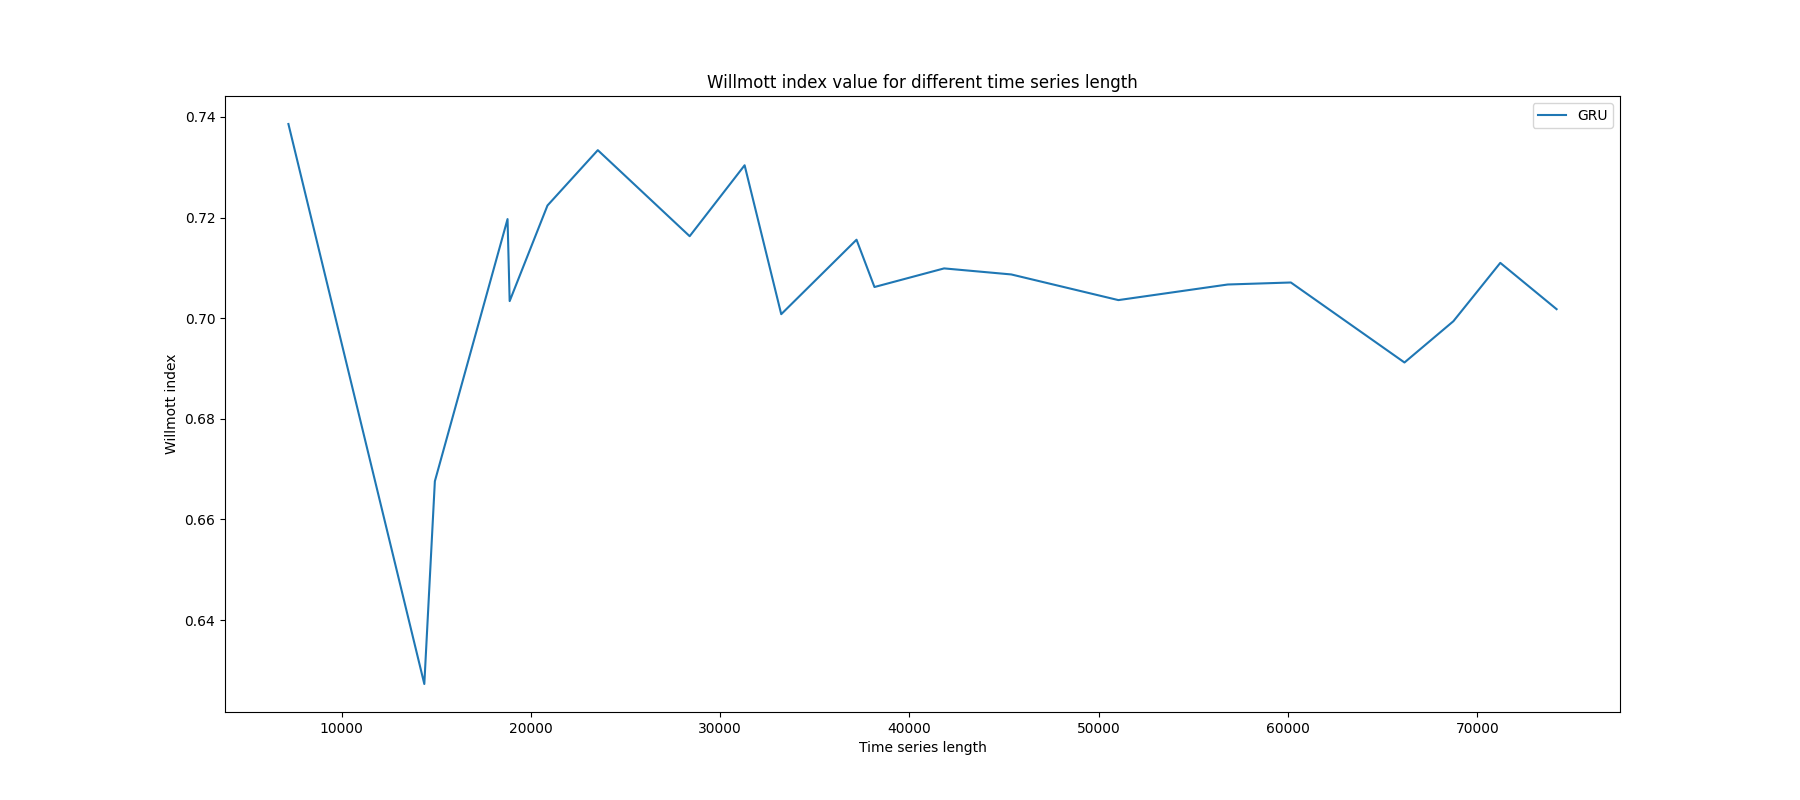
\includegraphics[scale=0.3]{cities_willmott.png}}
	\caption{Wartość indeksu Willmott'a w zależności od ilości analizowanych punktów pomiarowych}
	\label{figure:scale_willmott}
\end{figure}
\FloatBarrier

Podobnie jak w pozostałych przypadkach przedstawianych wyników samo zestawienie parametrów opisujących jakość wyników nie obrazuje w pełni obrazu analizowanej sytuacji. Zwłaszcza biorąc pod uwagę znaczenie przypisywane wynikowi testu $R^2$ w poprzednich przypadkach, jego fluktuacje mogą poddawać w wątpliwość skalowalność modelu. Wydaje się więc sensownym przeanalizowanie wizualizacji predykcji w celu próby wyłapania różnic w predykcjach. 

Zadanie to może być utrudnione poprzez losowy podział wejściowego szeregu na dane uczące i testujące. Otrzymane zestawienie wyników predykcji z danymi testującymi będzie różne dla różnych długości szeregu. Zadanie porównania dopasowania do zbioru testującego dla różnych długości szeregu zostało podjęte z wykorzystaniem wykresów dla względnie podobnych w kształcie zbiorów testujących. 

Wizualizacje te są prezentowane na \autoref{figure:scale_8} oraz \autoref{figure:scale_26}. Wyraźnie widoczna jest wspomniana różnica zbiorów testowych z obu rysunków. Nie wydaje się ona jednak tak duża, aby uniemożliwić poczynienie obserwacji odnośnie zachowania modelu dla obu szeregów czasowych.

Pomimo prawie czterokrotnego wzrostu długości szeregu nie widać drastycznych zmian w jakości uzyskiwanej predykcji. W obu przypadkach model zdaje się względnie poprawnie odwzorowywać dane testowe. Wydaje się to oznaczać poprawność przeprowadzonego badania, brak źle zbudowanych szeregów czasowych i odpowiednie przetwarzanie ich przez model. 

Można nawet odnieść wrażenie, że dla dłuższego szeregu czasowego model GRU lepiej przewiduje wartości. Przykładem może być tutaj zima z przełomu roku 2006 i 2007, gdzie przy większej ilości danych model bardzo mocno dopasowuje się do kształtu danych ze zbioru testującego. Trudno stwierdzić czy jest to faktycznie lepsza predykcja czy tylko wzrost ilości danych dla tego punktu czasowego ją lepiej uwidacznia. Biorąc pod uwagę odnotowany w \autoref{table:scale_comparison} spadek wartości błędu średniokwadratowego przy wzroście długości szeregu nie można wykluczyć możliwości nieco dokładniejszej predykcji dla liczniejszego szeregu. 

\begin{figure}[!ht]
	\centering
	\makebox[0pt]{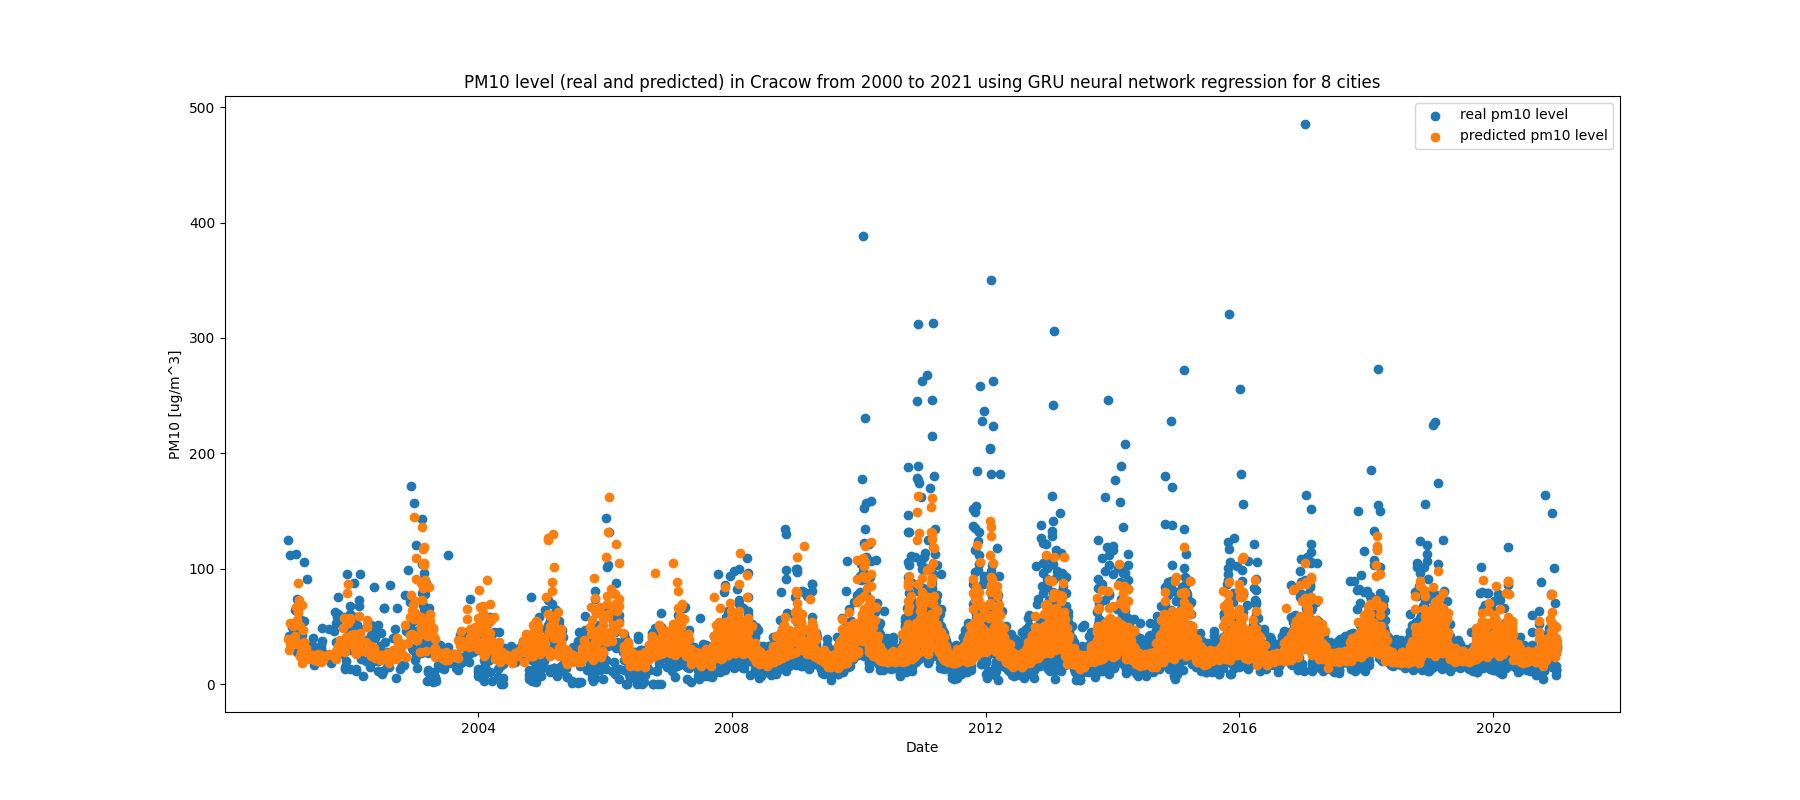
\includegraphics[scale=0.4]{scale_8.png}}
	\caption{Zestawienie wyników sieci neuronowej opartej na architekturze GRU dla 8 punktów pomiarowych}
	\label{figure:scale_8}
\end{figure}
\FloatBarrier

\begin{figure}[!ht]
	\centering
	\makebox[0pt]{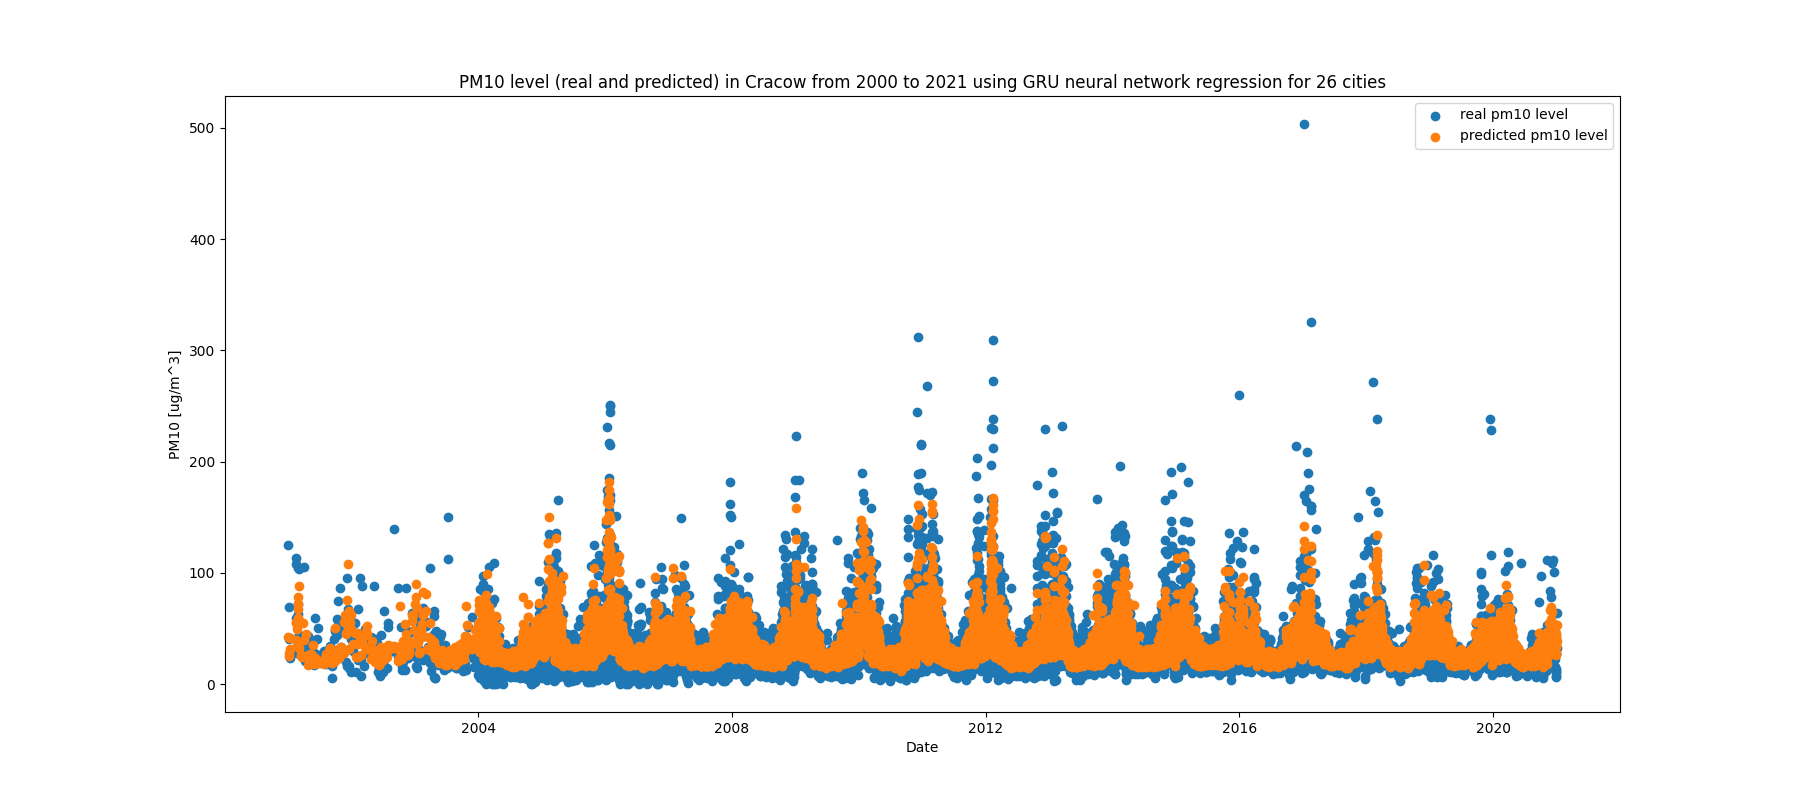
\includegraphics[scale=0.4]{scale_26.png}}
	\caption{Zestawienie wyników sieci neuronowej opartej na architekturze GRU dla 26 punktów pomiarowych}
	\label{figure:scale_26}
\end{figure}
\FloatBarrier

Przedstawione w tym podrozdziale wykresy oraz tabela porównawcza stanowią wystarczające podstawy do wyciągania dalej idących wniosków. Warto zauważyć trudność jednoznacznego określenia długości szeregu będącej limitem skalowalności modelu. Wszystkie czynniki płynące z wyników tego badania zostaną wzięte pod uwagę podczas formułowania wniosków w \hyperlink{section.6}{rozdziale 6}.

\newpage
\section{Wnioski}
W poprzednich rozdziałach przedstawione zostały badania przeprowadzone w celu określenia użyteczności rekurencyjnych sieci neuronowych do predykcji szeregów czasowych. Przybliżona została metodologia badań oraz uzyskane wyniki zostały przeanalizowane w celu zapewnienia podstaw do wyciągania dalszych wniosków. W ramach tego rozdziału wnioski te zostaną sformułowane i ugruntowane w otrzymanych wynikach. Zostaną również przedstawione kierunki potencjalnych dalszych badań mogących zwiększyć zrozumienie zagadnienia.

\subsection{Zasadność wykorzystania rekurencyjnych sieci neuronowych}
Podstawowym pytaniem stawianym w ramach tej pracy jest sensowność korzystania z rekurencyjnych sieci neuronowych do celów predykcyjnych jeżeli istnieją klasyczne, bardziej oczywiste metody. W celu umożliwienia osądu na ten temat warto wyciągnąć wnioski odnośnie jakości predykcji tych metod. Wnioski te mają starać się podkreślać ich silne i słabe strony, zastosowania dla których są one preferowane nad innymi metodami oraz inne aspekty umożliwiające wydanie ostatecznej opinii.

W trakcie badań z regresją liniową korzystając z metody najmniejszych kwadratów jasno ukazuje się jeden aspekt działania tej metody. Radzi sobie ona bardzo dobrze z dopasowywaniem się do ogólnych trendów, okresowości danych i dobrze odwzorowuje typowe elementy szeregu czasowego. Problemem tej metody jest natomiast przewidywanie elementów szeregu odbiegających od normy (bardzo wysokich poziomów zanieczyszczeń w ramach tej pracy). Można próbować wnioskować na tej podstawie, że istnieje pole do poprawy tej metody i nie jest ona na pewno najlepszym wyborem we wszystkich problemach predykcyjnych. 

Całkowicie inne wnioski płyną z analizy wykorzystania drzew decyzyjnych w celach predykcyjnych. Wyraźnie wybija się jej skłonność do zbytniego dopasowywania się do odbiegających od normy wartości szeregu czasowego. Przy braku nadzoru tendencja ta prowadzi do całkowicie niepoprawnych predykcji. Wyciągając wnioski na temat użyteczności tej metody opierając się tylko na badaniach przeprowadzonych w ramach tej pracy można stwierdzić, że drzewa decyzyjne słabo nadają się do takiego zastosowania. Istnieje oczywiście możliwość, że jest to niesprawiedliwy osąd i w innych przypadkach byłaby ona o wiele bardziej użyteczna.

Względem przydatności rekurencyjnych sieci neuronowych również mogą zostać wyciągnięte pewne ogólne spostrzeżenia. Oczywiście każda z badanych sieci ma różne właściwości i odmienne wnioski z nich płynące, których nie należy pomijać. Występują jednak podobieństwa między nimi tak znaczące, że można wysnuć kilka wniosków traktując je jako spójną całość bez niepotrzebnego usuwania niuansów pomiędzy nimi. Podejście takie może być bardzo przydatne, pamiętając pierwotne pytanie stawiane w ramach tej pracy - czy rekurencyjne sieci neuronowe są odpowiednie do przewidywania szeregów czasowych. Pozwoli ona odpowiedzieć na to pytanie bez niepotrzebnego roztrząsania niuansów rekurencyjnych sieci neuronowych. Niuanse te są oczywiście bardzo ważne, więc zostaną przedstawione w dalszej części tego rozdziału.

Patrząc na rekurencyjne sieci neuronowe jako całość można stwierdzić, że co do zasady dobrze oddają one zarówno typowe elementy szeregu jak i te bardziej nietypowe. Mają pewne problemy z wychwytywaniem długotrwałych trendów oraz nie przewidują bardzo dokładnie wyjątkowo wysokich wartości w szeregu. Można więc wnioskować, że radzą sobie adekwatnie w obu obszarach, nie kładąc szczególnego nacisku na żaden z nich. 

Na podstawie powyższych wniosków wydaje się możliwe zbudowanie odpowiedzi na pytanie czy wykorzystywanie rekurencyjnych sieci neuronowych do predykcji szeregów czasowych jest sensowne. Najbardziej poprawne wydaje się stwierdzenie, że zazwyczaj tak. Ważne jest jednak zrozumienie kwalifikatora zazwyczaj w tym wniosku, bo dobór metody do rozwiązania problemu powinien być uzależniony od rzeczonego problemu. W przypadkach, gdzie w szeregu nie występują wyraźne odstępstwa od normy, lepszym wyborem może okazać się klasyczna regresja liniowa na podstawie metody najmniejszych kwadratów. Radzi sobie ona lepiej w wyłapywaniu trendów i jest zdecydowanie mniej skomplikowana. Jeżeli jednak w procesie predykcyjnym ważne jest reagowanie na bardzo wysokie skoki wartości w szeregu czasowym to rekurencyjne sieci neuronowe są zdecydowanie lepszym wyborem. Widać więc wyraźnie, że w pewnych specyficznych przypadkach metody klasyczne osiągają lepsze wyniki, ale w większości przypadków zastosowanie rekurencyjnych sieci neuronowych jest lepszym wyborem. 

Warto zastanowić się nad znaczeniem tego wniosku dla praktycznych zastosowań predykcji szeregów czasowych. Bardzo rzadko zdarzają się problemy predykcyjne, w których nie jest ważna możliwość przewidzenia bardzo wysokiej wartości w szeregu czasowym. W przypadku wykorzystywanego w tej pracy szeregu opisującego poziom zanieczyszczenia powietrza łatwo ocenić wagę takiego przewidzenia. Wiedza z wyprzedzeniem pozwala na ostrzeżenie ludności o niebezpieczeństwie lub na próby zapobiegania. W Krakowie często w dniach wysokiego skażenia powietrza oferowana jest na przykład darmowa komunikacja miejska \cite{krkFreeMPK} w celu zachęcenia ludzi do rezygnacji z podróży samochodem przyczyniającym się do zanieczyszczenia. Przy trafnych predykcjach dotyczących zanieczyszczenia powietrza władze miasta otrzymują możliwość lepszego przygotowania się na wprowadzenie darmowej komunikacji z większym wyprzedzeniem. Przykład ten wyraźnie ilustruje korzyści płynące z możliwości przewidzenia problemu zanim on wystąpi, które można traktować w zasadzie uniwersalnie. 

Ciężko wyobrazić sobie przykład szeregu czasowego, który kompletnie ignoruje aspekt minimalizowania ryzyka w zjawisku, które opisuje. Na pewno szeregi takie istnieją, ale zdaje się poprawnym stwierdzenie, że jeżeli zjawisko jest wystarczająco ważne, żeby je monitorować i próbować przewidywać to istnieje pewien poziom zagrożenia z niego płynący. Wszelkie pomiary klimatyczne, monitorowanie rynków finansowych, wydajność produkcji, badania opinii publicznej oraz wiele więcej zjawisk układanych w szeregi czasowe uznaje za istotne zmniejszanie ryzyka wystąpienia poważnych problemów. 

Biorąc pod uwagę jak duża jest przewaga rekurencyjnych sieci neuronowych nad klasycznymi metodami w praktycznych, rzeczywistych zastosowaniach, przytaczanie innych przewag wydaje się zbyteczne. Biorąc pod uwagę spełnienie głównego celu predykcji szeregów czasowych, czyli umożliwianie podejmowania działań redukujących ryzyko płynące ze zjawiska opisywanego przez szereg, ciężko znaleźć ograniczenia mogące podważyć użyteczność sieci rekurencyjnych. Ze znaczącą dozą pewności można stwierdzić, że rekurencyjne sieci neuronowe są odpowiednie do przeprowadzania predykcji szeregów czasowych.

\subsection{Wykorzystanie rekurencyjnych sieci neuronowych}
W trakcie badań sporo uwagi poświęcone zostało wykorzystaniu różnych architektur rekurencyjnych sieci neuronowych do predykcji szeregów czasowych. W trakcie tych badań poczynione zostało wiele interesujących obserwacji mogących posłużyć do formułowania wniosków odnośnie użycia tych sieci. W ramach tego podrozdziału zostaną przedstawione te wnioski oraz ich zasadność w praktycznych zastosowaniach badanych sieci neuronowych. 

Różnice w uzyskiwanych wynikach nie były w żadnym wypadku radykalne, aczkolwiek nie należy ich pomijać podczas formułowania wniosków. Widoczny jest wzrost jakości wyników przy przejściach z prostej rekurencyjnej sieci neuronowej do sieci typu LSTM oraz potem do sieci GRU. Zbieżność kolejności powstawania tych architektur sieci ze wzrostem ich wyników nie jest przypadkowa. Można stwierdzić, że razem z rozwojem dziedziny rekurencyjnych sieci neuronowych, poprawiają się ich możliwości predykcyjne oraz jakość zwracanych wyników. Fakt ten był rozumiany w innych, bardziej typowych zastosowaniach tych sieci, ale występowanie takiej poprawy w zastosowaniach predykcyjnych pozwala optymistycznie patrzeć na dalszy rozwój tej dziedziny sztucznej inteligencji. 

Warte odnotowania jest kluczowe znaczenie doboru odpowiedniej wielkości warstwy rekurencyjnej do skali skomplikowania rozwiązywanego problemu. W ramach wstępnej analizy wyników znaczenie to zostało wyraźnie przedstawione i powinno być brane pod uwagę w trakcie prac z modelami predykcyjnymi opartymi na rekurencyjnych sieciach neuronowych. Podobnie jak przy przyglądaniu się jakości uzyskiwanych wyników, w tym aspekcie również widoczna była poprawa w nowszych architekturach. 

Mając na uwadze te czynniki można wysunąć wniosek, według którego używanie nowocześniejszych rekurencyjnych sieci neuronowych ma wyższą przydatność od tych nieco starszych rozwiązań. Wniosek ten jest ważny biorąc pod uwagę ciągle trwające badania rozwojowe tej dziedziny nauki. Często prezentowane są nowe architektury ulepszające działanie rekurencyjnych sieci neuronowych. Są one zazwyczaj ukierunkowane na inne wykorzystania niż predykcja szeregów czasowych. Jednak w ramach tej pracy wydaje się potwierdzać przekonanie, że ulepszenia te są równie widoczne w zastosowaniach predykcyjnych. 

Warto odnieść te spostrzeżenia do rzeczywistych zastosowań sieci rekurencyjnych w predykcji szeregów czasowych. Przy wyborze oparcia swojego modelu predykcyjnego na rekurencyjnych sieciach neuronowych można mieć przeświadczenie, że w niedalekiej przyszłości powstaną ulepszenia poprawiające jakość predykcji. W przypadku zanieczyszczenia powietrza analizowanego w ramach tej pracy daje to nadzieję na wytworzenie modelu jeszcze lepiej przygotowanego do wyszukiwania potencjalnych zagrożeń w szeregu. Zwiększająca się jakość predykcji pozwoli w przyszłości z większą pewnością podejmować działania ograniczające ryzyko nie martwiąc się o potencjalną fałszywość predykcji. Taka poprawa może również zminimalizować ilość sytuacji z wysokim poziomem zanieczyszczeń, które nie zostaną poprawnie przewidziane przez sieć neuronową. Nie wydaje się możliwym uzyskanie całkowitej pewności odnośnie otrzymywanych predykcji, ale wzrost tej pewności jest czynnikiem, który zdaje się usprawiedliwiać wykorzystywanie takich rozwiązań. 

Interesujące wnioski płyną również z badania skalowalności najnowocześniejszej sieci ujętej w tym badaniu, czyli Gated Recurrent Unit. Dziesięciokrotny wzrost długości szeregu nie miał negatywnego wpływu na wyniki predykcji. W pewnych kategoriach oceny widoczna była nawet poprawa wraz ze wzrostem ilości danych. Można na tej podstawie wnioskować, że sieć taka jest dobrze przygotowana na pracę z dużymi zbiorami danych i nie napotyka problemów z powodu skali problemu.

Wniosek ten może mieć bardzo duże znaczenia dla praktycznych zastosowań takich sieci. Obecnym trendem zdaje się zwiększanie liczby czujników monitorujących różne zjawiska, a co za tym idzie zwiększanie ilości danych na podstawie których można przewidywać wartości tych zjawisk w przyszłości. W wykorzystywanej tutaj bazie danych Głównego Inspektoratu Ochrony Środowiska ilość stacji pomiarowych wzrosła siedemnastokrotnie. Wyraźnie zwiększyła się również ilość monitorowanych substancji zanieczyszczających. Przy takim przyroście dostępnych danych, skalowalność modelu predykcyjnego będzie miała kluczowe znaczenie, bo ilość danych będzie ciągle rosnąć. Jest bardzo prawdopodobne, że sieci neuronowe mają limit tego jak bardzo można zwiększyć skalę problemu bez utraty jakości wyników, ale zdaje się ona zadowalająco wysoka. Zatem w świecie większej ilości punktów pomiarowych, czujników działających w metodologii ,,internetu rzeczy'' fakt, że sieć GRU radzi sobie adekwatnie ze wzrostem skali może mieć bardzo duże znaczenie.

\subsection{Dalsze kierunki badań}
W ramach tej pracy przeprowadzone zostało wiele badań pozwalających ocenić użyteczność rekurencyjnych sieci neuronowych do predykcji szeregów czasowych. Temat ten nie został jednak wyczerpany i istnieje wiele kierunków, które mogą obrać przyszłe badania. W tym podrozdziale przedstawione zostanie kilka takich kierunków z wyjaśnieniem jakie potencjalne korzyści mogą one przynieść. 

Pierwszym obszarem badań, którego kontynuacja może przynieść interesujące wyniki jest badanie skalowalności sieci w architekturze Gated Recurrent Unit. Najpewniej istnieje granica skali problemu, której przekroczenie spowoduje wyraźny spadek jakości predykcji. W ramach tej pracy nie została ona jednak odnaleziona z powodu braku dostatecznej ilości danych. Podjęcie prób znalezienia tej granicy może pozwolić na lepsze zrozumienie tego aspektu sieci neuronowych. Znaczenie takiego odkrycia jest tym większe, że jak wywnioskowano wcześniej może mieć to wpływ na przydatność tej metody predykcyjnej w realnym świecie. 

W ramach tej pracy wyciągnięte zostały wnioski odnośnie ogólnej przydatności rekurencyjnych sieci neuronowych do predykcji większości szeregów czasowych. Wydaje się odpowiednim przeprowadzenie większej ilości badań na różnych szeregach, aby umocnić lub obalić ten wniosek. Istnieje pewne prawdopodobieństwo, że wyciągnięte wnioski zależą w pewnej mierze od specyficznego szeregu czasowego stworzonego na potrzeby tej pracy. Powtórzenie tych badań dla innych szeregów zdaje się więc umożliwić wyeliminowanie lub przynajmniej wyraźne zredukowanie tego prawdopodobieństwa. 

W \hyperlink{subsection.6.2}{podrozdziale 6.2} zauważono również poprawę wyników przy korzystaniu z bardziej nowoczesnych architektur rekurencyjnych sieci neuronowych. Wydaje się więc interesujące przeprowadzenie podobnych badań jak w tej pracy, ale z wykorzystaniem jeszcze bardziej nowoczesnych sieci. Przykładem takiej sieci, która nie jest ujęta w ramach tego badania jest sieć Content-Adaptive Recurrent Unit zaproponowana w 2020 roku \cite{chan2020caru}. Sieć ta obecnie nie jest zaimplementowana w najpopularniejszych bibliotekach i dlatego nie została uwzględniona w tym badaniu. Jednak przydatność CARU i innych jeszcze nie powstałych sieci może być bardzo interesującym kierunkiem badań w przyszłości. 

\newpage
\printbibliography[title=Bibliografia]

\end{document}